%%%%%%%%%%%%%%%%%%%%%%%%%%%%%%%%%%%%%%%%%%%%%%%%%%%%%%%%%%%%%%%%%%%%%%%%%%%%%%%%
%%% Benutzer-Einstellungen %%%%%%%%%%%%%%%%%%%%%%%%%%%%%%%%%%%%%%%%%%%%%%%%%%%%%
%%%%%%%%%%%%%%%%%%%%%%%%%%%%%%%%%%%%%%%%%%%%%%%%%%%%%%%%%%%%%%%%%%%%%%%%%%%%%%%%
%%                                                                      %%%%%%%%
%      Einstellungen erfolgen in der Datei Einstellungen.tex             %%%%%%%
       %%%%%%%%%%%%%%%%%%%%%%%%%%%%%%%%%%%%%%%%%%%%%%%%%%%%%%%%%%%%%%%%%%%%%%%%%%%%%%%%
%%% DATEI-INFO %%%%%%%%%%%%%%%%%%%%%%%%%%%%%%%%%%%%%%%%%%%%%%%%%%%%%%%%%%%%%%%%%
%%%%%%%%%%%%%%%%%%%%%%%%%%%%%%%%%%%%%%%%%%%%%%%%%%%%%%%%%%%%%%%%%%%%%%%%%%%%%%%%
%%% In dieser Datei werden alle wichtigen Einstellungen der Vorlage gesetzt %%%%
%%% Hier darfst du Werte ändern ;-) %%%%%%%%%%%%%%%%%%%%%%%%%%%%%%%%%%%%%%%%%%%%
%%%%%%%%%%%%%%%%%%%%%%%%%%%%%%%%%%%%%%%%%%%%%%%%%%%%%%%%%%%%%%%%%%%%%%%%%%%%%%%%
%
%%%%%%%%%%%%%%%%%%%%%%%%%%%%%%%%%%%%%%%%%%%%%%%%%%%%%%%%%%%%%%%%%%%%%%%%%%%%%%%%
%%%%%%%%%%%%%%%%%%%%%%%%%%%%%%%%%%%%%%%%%%%%%%%%%%%%%%%%%%%%%%%%%%%%%%%%%%%%%%%%
\ifx\inPreamble\undefined \else %%%% 'MAGIC' %%%%%%%%%%%%%%%%%%%%%%%%%%%%%%%%%%%
%%%%%%%%%%%%%%%%%%%%%%%%%%%%%%%%%%%%%%%%%%%%%%%%%%%%%%%%%%%%%%%%%%%%%%%%%%%%%%%%
%%%%%%%%%%%%%%%%%%%%%%%%%%%%%%%%%%%%%%%%%%%%%%%%%%%%%%%%%%%%%%%%%%%%%%%%%%%%%%%%
%%%%%%% Pflicht-Einstellungen %%%%%%%%%%%%%%%%%%%%%%%%%%%%%%%%%%%%%%%%%%%%%%%%%%

% Bachelor-Thesis, Master-Thesis
\newcommand{\artderarbeit}{Master-Thesis}

% Thema der Thesis (wie in der Aufgabenstellung)
\newcommand{\thema}{Accelerating the computation of the matrix sign function}


% Gibt es eine Verlängerung der Bearbeitungszeit?
\setbool{verlaengerung}{false}
% Wenn ja, hier auf "true" setzen und die Datei Verlaengerung.pdf ersetzen

% Eine optionale Danksagung kann in der Datei "Danksagung.tex" formuliert werden
\setbool{danksagung}{false}

% Euer voller Name
\newcommand{\autor}{Jay Karippacheril Jacob}

% Eure Matrikelnummer
\newcommand{\matrikelnummer}{2130800}

% Offizielle Bezeichnung des Studiengangs
\newcommand{\studiengang}{Computer Simulation in Science}

% Wenn es in Eurem Studiengang keine Schwerpunkte gibt einfach leer lassen
\newcommand{\schwerpunkt}{Computational Fluid Mechanics}

% Der Lehrstuhl, an dem die Thesis geschrieben wird
\newcommand{\lehrstuhl}{Department of Mathematics and Natural Sciences}

% Betreuer? (falls mehrere: mit \\ trennen)
%\newcommand{\betreuer}{Vorname Nachname M.Sc.}

% Erstprüfer (siehe Anmeldung)
%\newcommand{\prueferA}{Prof. Dr. Andreas Frommer}

% Zweitprüfer (siehe Anmeldung)
%\newcommand{\prueferB}{Dr. Gustavo Alonso Ramirez Hidalgo}


% Euer Abgabedatum
\newcommand{\abgabedatum}{03. December 2024}

% Ort
\newcommand{\ort}{Wuppertal}

% Schlagwörter, mit denen man das PDF finden kann
\newcommand{\schlagwoerter}{Thesis, Master, Bergische Universität Wuppertal}


%%% Ende der Pflicht-Einstellungen %%%%%%%%%%%%%%%%%%%%%%%%%%%%%%%%%%%%%%%%%%%%%
%%%%%%%%%%%%%%%%%%%%%%%%%%%%%%%%%%%%%%%%%%%%%%%%%%%%%%%%%%%%%%%%%%%%%%%%%%%%%%%%

%%%%%%%%%%%%%%%%%%%%%%%%%%%%%%%%%%%%%%%%%%%%%%%%%%%%%%%%%%%%%%%%%%%%%%%%%%%%%%%%
%%% Layout-Anpassung (Optional) %%%%%%%%%%%%%%%%%%%%%%%%%%%%%%%%%%%%%%%%%%%%%%%%

%%% Zweiseitiges Layout
\setbool{doppelseitig}{true}			% Einseitiger oder doppelseitiger Druck?

%%% Hyperlinks
\setbool{linksMarkieren}{true}			% Anklickbare Links im PDF-Dokument markieren?


%%%%%%%%%%%%%%%%%%%%%%%%%%%%%%%%%%%%%%%%%%%%%%%%%%%%%%%%%%%%%%%%%%%%%%%%%%%%%%%%
%%% Verzeichnisse %%%%%%%%%%%%%%%%%%%%%%%%%%%%%%%%%%%%%%%%%%%%%%%%%%%%%%%%%%%%%%

\setbool{abbildungsverzeichnis}{true} 	% Abbildungsverzeichnis erzeugen?
\setbool{quellcodeverzeichnis}{true}	% Quellcodeverzeichnis erzeugen?
\setbool{tabellenverzeichnis}{true}		% Tabellenverzeichnis erzeugen?
\setbool{symbolverzeichnis}{false}		% Symbolverzeichnis erzeugen?
\setbool{akronymverzeichnis}{false}		% Akronymverzeichnis erzeugen?
\setbool{abkuerzungsverzeichnis}{false}	% Abkürzungsverzeichnis erzeugen?
\setbool{glossar}{true}					% Glossar erzeugen?

\setbool{verzeichnisseImInhaltsverzeichnis}{true} % Verzeichnisse im Inhaltsverzeichnis erwähnen?

\setbool{verzeichnisseZusammenfassen}{true} % Seitenumbruch zwischen den Verzeichnissen deaktivieren?


%%%%%%%%%%%%%%%%%%%%%%%%%%%%%%%%%%%%%%%%%%%%%%%%%%%%%%%%%%%%%%%%%%%%%%%%%%%%%%%%
%%% Kapitelnummerierung %%%%%%%%%%%%%%%%%%%%%%%%%%%%%%%%%%%%%%%%%%%%%%%%%%%%%%%%

\newcommand\kapitelTiefeNummerierung{3} 	  % Wie tief soll nummeriert werden?
\newcommand\kapitelTiefeInhaltsverzeichnis{2} % Bis zu welcher Tiefe sollen die Einträge ins Inhaltsverzeichnis?

% Tiefe Bedeutung
% 0     \chapter
% 1     \section
% 2     \subsection
% 3     \subsubsection
% 4     \paragraph
% 5     \subparagraph


%%% Zusatzerklärung

\setbool{zusatzErklaerung}{false} 		% Hiermit können zusätzliche Erklärungen eingebunden werden (siehe Zusatzerklaerung.tex, wird im Normalfall nicht benötigt)


%%%%%%%%%%%%%%%%%%%%%%%%%%%%%%%%%%%%%%%%%%%%%%%%%%%%%%%%%%%%%%%%%%%%%%%%%%%%%%%%
%%% Farben (Optional) %%%%%%%%%%%%%%%%%%%%%%%%%%%%%%%%%%%%%%%%%%%%%%%%%%%%%%%%%%

\setbool{color}{true} % Farbe für Design-Elemente verwenden (true/false)

\newcommand{\colormodel}{cmyk} % z.B. cmyk, rgb oder gray
% Falls das Tool eurer Druckerei Schwarz-Weiß-Seiten trotz \setbool{color}{false}
% _fälschlicherweise_ als Farbseiten erkennt (das kann ziemlich teuer werden!), 
% könnt ihr hier das Farbmodell der Vorlage umstellen.
%
% So hatten wir schon einmal den Fall, dass eine Thesis-Druckerei die S/W-Seiten
% erst korrekt erkannt hat, wenn das (eigentlich für das Drucken ungeeignete)
% RGB-Modell verwendet wurde...
% 
% Bilder und eingebundene PDFs werden durch diese Einstellung nicht geändert!
%
% Ein paar Beispiele für sinnvolle Werte:
% {cmyk}  - CMYK (Cyan, Magenta, Yellow, Key) ist _das Farbmodell_ für alles was gedruckt wird.
%           Jede professionelle Druckerei kann damit umgehen!
%           => der Standard bei Drucksachen und daher auch in dieser Vorlage
%
% {rgb}   - RGB (Red, Green, Blue) ist ein Farbmodell für Bildschirme etc.
%           Im Gegensatz zum Druck mit Pigmenten (=subtraktive Farbmischung) wird
%           hier mit Licht gearbeitet (Additive Farbmischung). RGB ist daher nicht
%           für den Druck geeignet und wird vor dem Druckvorgang in ein anderes
%           Farbmodell (z.B. CMYK) umgewandelt.
%           => eigentlich falsch, wird in Einzelfällen aber von Druckereien angefordert
%
% {gray}  - Wer möchte, kann auch das Farbmodell "gray" verwenden. Dann werden alle
%           Farben direkt in Graustufen umgerechnet.
%           In diesem Fall wird zusätzlich \setbool{color}{false} empfohlen.
%           So wird die Darstellung von Quelltexten an die nun fehlenden Farben angepasst.
%
% Weblinks zum Thema:
% https://de.wikipedia.org/wiki/CMYK-Farbmodell
% https://de.wikipedia.org/wiki/RGB-Farbraum
% https://www.ctan.org/pkg/xcolor

%%%%%%%%%%%%%%%%%%%%%%%%%%%%%%%%%%%%%%%%%%%%%%%%%%%%%%%%%%%%%%%%%%%%%%%%%%%%%%%%
%%% Seitenränder %%%%%%%%%%%%%%%%%%%%%%%%%%%%%%%%%%%%%%%%%%%%%%%%%%%%%%%%%%%%%%%

\setlength{\bindekorrektur}{1.0cm}
% Wie breit ist der Teil, an dem die einzelnen Blätter 
% mit einander verklebt/anderweitig verbunden werden?

\setlength{\randAussen}{%
	\ifbool{doppelseitig}{%
		2.50cm% 2.5 - 3.4cm (bei doppelseitigem Layout)
	}{%
		1.88cm% 1.88 - 2.5cm (bei einseitigem Layout)
	}%
} 
% Wie viel Rand außen neben dem Text (einseitig: wie viel Rand rechts neben dem Text)
% Innerer bzw. linker Rand wird daraus automatisch berechnet



%%%%%%%%%%%%%%%%%%%%%%%%%%%%%%%%%%%%%%%%%%%%%%%%%%%%%%%%%%%%%%%%%%%%%%%%%%%%%%%%
%%% Literatur-Anpassung (Optional) %%%%%%%%%%%%%%%%%%%%%%%%%%%%%%%%%%%%%%%%%%%%%

% Es gibt drei Arten von Quellen:
%
% Gruppe A : Quellen, die im Text mit \cite{...} zitiert wurden
% Gruppe B : Quellen, die mit \nocite{...} markiert wurden (und sonst nicht zitiert wurden)
% Gruppe C : Quellen, die gar nicht zitiert wurden

\setbool{nichtZitiertInweiterfuehrendeLiteratur}{false}
% nicht zitierte Quellen automatisch mit \nocite{} aufnehmen?
% => d.h. Gruppe C wird automatisch in Gruppe B verschoben 
% => ansonsten wird stattdessen \explizitesNocite aktiv

\setbool{weiterfuehrendeLiteratur}{true}
% Separates Verzeichnis für weiterführende Literatur?
%
% "true": Separates Verzeichnis "Weiterführende Literatur" erstellen
%   Gruppe A => "Literatur"
%   Gruppe B => "Weiterführende Literatur"
% 
% "false": Alles landet in "Literatur"
%   Gruppe A => "Literatur"
%   Gruppe B => "Literatur"

\newcommand{\explizitesNocite}{%
% Wenn bei der Literatur Gruppe B manuell festgelegt werden soll, kann dies hier geschehen:
	\nocite{ARM:AMBA4AXI4StreamProtocol:v1_0}
	\nocite{ARM:AMBA_AXI_and_ACE_Protocol_Specification:E}
	\nocite{AnalogDevices:ADAU1761:rev_C}
	\nocite{Book:PerceptionBasedDataprocessingInAcoustics}
	\nocite{Philips:I2S_BUS_Specification}
	\nocite{Xilinx:PG021:v7_1}
	\nocite{Xilinx:UG473:v1_11}
	\nocite{Xilinx:UG761:v13_1}
	\nocite{Xilinx:UG901:v2016_2}
	\nocite{Xilinx:UG906:v2016_2}
	\nocite{Xilinx:WP231}
	\nocite{Xilinx:XAPP1206:v1_1}
	\nocite{Xilinx:PG109:v9_0}
	\nocite{ARM:NEONProgrammersGuide:v1_0}
	\nocite{Book:TheScientistandEngineersGuidetoDigitalSignalProcessing}
	\nocite{IEEE:754:2008}
	\nocite{SpectrumAndSpectralDensityEstimationByTheDFTincludingAListOfWindowFunctions}
	% ... weitere Quellen ...
}

\setbool{alleAutorenExplizitNennen}{true} % Steuert die Nennung der Autoren im Literaturverzeichnis
% Hier gibt es zwei übliche Varianten:
% true  : Es werden immer alle Autoren genannt.
% false : Bis zu vier Autoren werden mit Namen genannt.
%           Gibt es mehr Autoren, werden die ersten drei genannt und
%           der Rest mit et al. abgekürzt (wie auch im Zitierschlüssel)

%%%%%%%%%%%%%%%%%%%%%%%%%%%%%%%%%%%%%%%%%%%%%%%%%%%%%%%%%%%%%%%%%%%%%%%%%%%%%%%%
%%% Sprach-Anpassung (Optional) %%%%%%%%%%%%%%%%%%%%%%%%%%%%%%%%%%%%%%%%%%%%%%%%
% Eine Liste der mögliche Sprachen finden sich in der Dokumentation zum LaTeX-Paket 'babel'
\newcommand{\hauptsprache}{english} % Sprache, in der das Dokument geschrieben ist. Wird auch für die Verzeichnisnamen etc. verwendet
\newcommand{\weitereSprachen}{ngerman, english, french}% weitere Sprachen, auf die kurzfristig mit \selectlanguage{language} gewechselt wird. (Wenn es mehrere sind werden diese mit Kommata getrennt)

% ngerman - Deutsch nach neuer Rechtschreibung
% english - Englisch
% french - Französisch

%%%%%%%%%%%%%%%%%%%%%%%%%%%%%%%%%%%%%%%%%%%%%%%%%%%%%%%%%%%%%%%%%%%%%%%%%%%%%%%%
\fi %%%%%%%%%%%%%%%%%%%%%%%%%%%%%%%%%%%%%%%%%%%%%%%%%%%%%%%%%%%%%%%%%%%%%%%%%%%%
%%%%%%%%%%%%%%%%%%%%%%%%%%%%%%%%%%%%%%%%%%%%%%%%%%%%%%%%%%%%%%%%%%%%%%%%%%%%%%%%                                          %%%%%%
%                                                                        %%%%%%%
%%                                                                      %%%%%%%%
%%%%%%%%%%%%%%%%%%%%%%%%%%%%%%%%%%%%%%%%%%%%%%%%%%%%%%%%%%%%%%%%%%%%%%%%%%%%%%%%
%%%%%%%%%%%%%%%%%%%%%%%%%%%%%%%%%%%%%%%%%%%%%%%%%%%%%%%%%%%%%%%%%%%%%%%%%%%%%%%%
%%%%%%%%%%%%%%%%%%%%%%%%%%%%%%%%%%%%%%%%%%%%%%%%%%%%%%%%%%%%%%%%%%%%%%%%%%%%%%%%
%%%%%%%%%%%%%%%%%%%%%%%%%%%%%%%%%%%%%%%%%%%%%
%%% ! WARNUNG ! %%%%%%%%%%%%%%%%%%%%%%%%%%%%%
%%%%%%%%%%%%%%%%%%%%%%%%%%%%%%%%%%%%%%%%%%%%%
%%%  Diese Datei bitte nur bearbeiten,    %%%
%%%   wenn du ein LaTeX-Experte bist      %%%
%%%             U N D                     %%%
%%%  die Vorlage unbedingt ändern willst  %%%
%%%%%%%%%%%%%%%%%%%%%%%%%%%%%%%%%%%%%%%%%%%%%
%%%%%%%%%%%%%%%%%%%%%%%%%%%%%%%%%%%%%%%%%%%%%
%
%%%%%%%%%%%%%%%%%%%%%%%%%%%%%%%%%%%%%%%%%%%%%%%%%%%%%%%%%%%%%%%%%%%%%%%%%%%%%%%%
%%% DATEI-INFO %%%%%%%%%%%%%%%%%%%%%%%%%%%%%%%%%%%%%%%%%%%%%%%%%%%%%%%%%%%%%%%%%
%%%%%%%%%%%%%%%%%%%%%%%%%%%%%%%%%%%%%%%%%%%%%%%%%%%%%%%%%%%%%%%%%%%%%%%%%%%%%%%%
%%% Diese Datei richtet diverse Pakete und Befehle für die Vorlage ein %%%%%%%%%
%%%%%%%%%%%%%%%%%%%%%%%%%%%%%%%%%%%%%%%%%%%%%%%%%%%%%%%%%%%%%%%%%%%%%%%%%%%%%%%%
%
\def\inPreamble{}% Flag setzen: wird sind in der Präambel
%%%%%%%%%%%%%%%%%%%%%%%%%%%%%%%%%%%%%%%%%%%%%%%%%%%%%%%%%%%%%%%%%%%%%%%%%%%%%%%%
%%% Encoding %%%%%%%%%%%%%%%%%%%%%%%%%%%%%%%%%%%%%%%%%%%%%%%%%%%%%%%%%%%%%%%%%%%

\RequirePackage[utf8]{inputenc}
% UTF8 Codierte .tex-Dateien

\RequirePackage[T1]{fontenc}
% Benutzung der europäischen Schriftkodierung
% z.B. zur richtigen Darstellung von Umlauten


%%%%%%%%%%%%%%%%%%%%%%%%%%%%%%%%%%%%%%%%%%%%%%%%%%%%%%%%%%%%%%%%%%%%%%%%%%%%%%%%
%%% Werkzeuge %%%%%%%%%%%%%%%%%%%%%%%%%%%%%%%%%%%%%%%%%%%%%%%%%%%%%%%%%%%%%%%%%%

\RequirePackage{etoolbox}		% Einfacheres Programmieren in LaTeX
\RequirePackage{calculator}		% Rechnen (auch mit Längen)
\RequirePackage{xfp}			% Genaueres Rechnen (aber nicht mit Längen)
\RequirePackage{pbox}			% \pbox (Parbox flexibler Breite)


%%%%%%%%%%%%%%%%%%%%%%%%%%%%%%%%%%%%%%%%%%%%%%%%%%%%%%%%%%%%%%%%%%%%%%%%%%%%%%%%
%%% Variablen zur Anpassung durch den Benutzer %%%%%%%%%%%%%%%%%%%%%%%%%%%%%%%%%
%%%%%%%%%%%%%%%%%%%%%%%%%%%%%%%%%%%%%%%%%%%%%%%%%%%%%%%%%%%%%%%%%%%%%%%%%%%%%%%%
%%% >>> werden gesetzt in der Datei "PersoenlicheAngaben.tex" %%%%%%%%%%%%%%%%%%

\newbool{abbildungsverzeichnis}
\newbool{quellcodeverzeichnis}
\newbool{tabellenverzeichnis}
\newbool{symbolverzeichnis}
\newbool{akronymverzeichnis}
\newbool{abkuerzungsverzeichnis}
\newbool{glossar}

\newbool{verzeichnisseZusammenfassen}
\newbool{verzeichnisseImInhaltsverzeichnis}

\newbool{nichtZitiertInweiterfuehrendeLiteratur}
\newbool{weiterfuehrendeLiteratur}
\newbool{alleAutorenExplizitNennen}

\newbool{verlaengerung}
\newbool{danksagung}
\newbool{zusatzErklaerung}

\newbool{color}
\newbool{linksMarkieren}

\newbool{doppelseitig}

\newlength{\bindekorrektur}
\setlength{\bindekorrektur}{1cm}

\newlength{\randAussen}
\setlength{\randAussen}{1.88cm} % 1.88 - 2.5cm (einseitig), 2.5 - 3.4 cm (doppelseitig)


%%%%%%%%%%%%%%%%%%%%%%%%%%%%%%%%%%%%%%%%%%%%%%%%%%%%%%%%%%%%%%%%%%%%%%%%%%%%%%%%
%%% Benutzer-Einstellungen anwenden %%%%%%%%%%%%%%%%%%%%%%%%%%%%%%%%%%%%%%%%%%%%

%%%%%%%%%%%%%%%%%%%%%%%%%%%%%%%%%%%%%%%%%%%%%%%%%%%%%%%%%%%%%%%%%%%%%%%%%%%%%%%%
%%% DATEI-INFO %%%%%%%%%%%%%%%%%%%%%%%%%%%%%%%%%%%%%%%%%%%%%%%%%%%%%%%%%%%%%%%%%
%%%%%%%%%%%%%%%%%%%%%%%%%%%%%%%%%%%%%%%%%%%%%%%%%%%%%%%%%%%%%%%%%%%%%%%%%%%%%%%%
%%% In dieser Datei werden alle wichtigen Einstellungen der Vorlage gesetzt %%%%
%%% Hier darfst du Werte ändern ;-) %%%%%%%%%%%%%%%%%%%%%%%%%%%%%%%%%%%%%%%%%%%%
%%%%%%%%%%%%%%%%%%%%%%%%%%%%%%%%%%%%%%%%%%%%%%%%%%%%%%%%%%%%%%%%%%%%%%%%%%%%%%%%
%
%%%%%%%%%%%%%%%%%%%%%%%%%%%%%%%%%%%%%%%%%%%%%%%%%%%%%%%%%%%%%%%%%%%%%%%%%%%%%%%%
%%%%%%%%%%%%%%%%%%%%%%%%%%%%%%%%%%%%%%%%%%%%%%%%%%%%%%%%%%%%%%%%%%%%%%%%%%%%%%%%
\ifx\inPreamble\undefined \else %%%% 'MAGIC' %%%%%%%%%%%%%%%%%%%%%%%%%%%%%%%%%%%
%%%%%%%%%%%%%%%%%%%%%%%%%%%%%%%%%%%%%%%%%%%%%%%%%%%%%%%%%%%%%%%%%%%%%%%%%%%%%%%%
%%%%%%%%%%%%%%%%%%%%%%%%%%%%%%%%%%%%%%%%%%%%%%%%%%%%%%%%%%%%%%%%%%%%%%%%%%%%%%%%
%%%%%%% Pflicht-Einstellungen %%%%%%%%%%%%%%%%%%%%%%%%%%%%%%%%%%%%%%%%%%%%%%%%%%

% Bachelor-Thesis, Master-Thesis
\newcommand{\artderarbeit}{Master-Thesis}

% Thema der Thesis (wie in der Aufgabenstellung)
\newcommand{\thema}{Accelerating the computation of the matrix sign function}


% Gibt es eine Verlängerung der Bearbeitungszeit?
\setbool{verlaengerung}{false}
% Wenn ja, hier auf "true" setzen und die Datei Verlaengerung.pdf ersetzen

% Eine optionale Danksagung kann in der Datei "Danksagung.tex" formuliert werden
\setbool{danksagung}{false}

% Euer voller Name
\newcommand{\autor}{Jay Karippacheril Jacob}

% Eure Matrikelnummer
\newcommand{\matrikelnummer}{2130800}

% Offizielle Bezeichnung des Studiengangs
\newcommand{\studiengang}{Computer Simulation in Science}

% Wenn es in Eurem Studiengang keine Schwerpunkte gibt einfach leer lassen
\newcommand{\schwerpunkt}{Computational Fluid Mechanics}

% Der Lehrstuhl, an dem die Thesis geschrieben wird
\newcommand{\lehrstuhl}{Department of Mathematics and Natural Sciences}

% Betreuer? (falls mehrere: mit \\ trennen)
%\newcommand{\betreuer}{Vorname Nachname M.Sc.}

% Erstprüfer (siehe Anmeldung)
%\newcommand{\prueferA}{Prof. Dr. Andreas Frommer}

% Zweitprüfer (siehe Anmeldung)
%\newcommand{\prueferB}{Dr. Gustavo Alonso Ramirez Hidalgo}


% Euer Abgabedatum
\newcommand{\abgabedatum}{03. December 2024}

% Ort
\newcommand{\ort}{Wuppertal}

% Schlagwörter, mit denen man das PDF finden kann
\newcommand{\schlagwoerter}{Thesis, Master, Bergische Universität Wuppertal}


%%% Ende der Pflicht-Einstellungen %%%%%%%%%%%%%%%%%%%%%%%%%%%%%%%%%%%%%%%%%%%%%
%%%%%%%%%%%%%%%%%%%%%%%%%%%%%%%%%%%%%%%%%%%%%%%%%%%%%%%%%%%%%%%%%%%%%%%%%%%%%%%%

%%%%%%%%%%%%%%%%%%%%%%%%%%%%%%%%%%%%%%%%%%%%%%%%%%%%%%%%%%%%%%%%%%%%%%%%%%%%%%%%
%%% Layout-Anpassung (Optional) %%%%%%%%%%%%%%%%%%%%%%%%%%%%%%%%%%%%%%%%%%%%%%%%

%%% Zweiseitiges Layout
\setbool{doppelseitig}{true}			% Einseitiger oder doppelseitiger Druck?

%%% Hyperlinks
\setbool{linksMarkieren}{true}			% Anklickbare Links im PDF-Dokument markieren?


%%%%%%%%%%%%%%%%%%%%%%%%%%%%%%%%%%%%%%%%%%%%%%%%%%%%%%%%%%%%%%%%%%%%%%%%%%%%%%%%
%%% Verzeichnisse %%%%%%%%%%%%%%%%%%%%%%%%%%%%%%%%%%%%%%%%%%%%%%%%%%%%%%%%%%%%%%

\setbool{abbildungsverzeichnis}{true} 	% Abbildungsverzeichnis erzeugen?
\setbool{quellcodeverzeichnis}{true}	% Quellcodeverzeichnis erzeugen?
\setbool{tabellenverzeichnis}{true}		% Tabellenverzeichnis erzeugen?
\setbool{symbolverzeichnis}{false}		% Symbolverzeichnis erzeugen?
\setbool{akronymverzeichnis}{false}		% Akronymverzeichnis erzeugen?
\setbool{abkuerzungsverzeichnis}{false}	% Abkürzungsverzeichnis erzeugen?
\setbool{glossar}{true}					% Glossar erzeugen?

\setbool{verzeichnisseImInhaltsverzeichnis}{true} % Verzeichnisse im Inhaltsverzeichnis erwähnen?

\setbool{verzeichnisseZusammenfassen}{true} % Seitenumbruch zwischen den Verzeichnissen deaktivieren?


%%%%%%%%%%%%%%%%%%%%%%%%%%%%%%%%%%%%%%%%%%%%%%%%%%%%%%%%%%%%%%%%%%%%%%%%%%%%%%%%
%%% Kapitelnummerierung %%%%%%%%%%%%%%%%%%%%%%%%%%%%%%%%%%%%%%%%%%%%%%%%%%%%%%%%

\newcommand\kapitelTiefeNummerierung{3} 	  % Wie tief soll nummeriert werden?
\newcommand\kapitelTiefeInhaltsverzeichnis{2} % Bis zu welcher Tiefe sollen die Einträge ins Inhaltsverzeichnis?

% Tiefe Bedeutung
% 0     \chapter
% 1     \section
% 2     \subsection
% 3     \subsubsection
% 4     \paragraph
% 5     \subparagraph


%%% Zusatzerklärung

\setbool{zusatzErklaerung}{false} 		% Hiermit können zusätzliche Erklärungen eingebunden werden (siehe Zusatzerklaerung.tex, wird im Normalfall nicht benötigt)


%%%%%%%%%%%%%%%%%%%%%%%%%%%%%%%%%%%%%%%%%%%%%%%%%%%%%%%%%%%%%%%%%%%%%%%%%%%%%%%%
%%% Farben (Optional) %%%%%%%%%%%%%%%%%%%%%%%%%%%%%%%%%%%%%%%%%%%%%%%%%%%%%%%%%%

\setbool{color}{true} % Farbe für Design-Elemente verwenden (true/false)

\newcommand{\colormodel}{cmyk} % z.B. cmyk, rgb oder gray
% Falls das Tool eurer Druckerei Schwarz-Weiß-Seiten trotz \setbool{color}{false}
% _fälschlicherweise_ als Farbseiten erkennt (das kann ziemlich teuer werden!), 
% könnt ihr hier das Farbmodell der Vorlage umstellen.
%
% So hatten wir schon einmal den Fall, dass eine Thesis-Druckerei die S/W-Seiten
% erst korrekt erkannt hat, wenn das (eigentlich für das Drucken ungeeignete)
% RGB-Modell verwendet wurde...
% 
% Bilder und eingebundene PDFs werden durch diese Einstellung nicht geändert!
%
% Ein paar Beispiele für sinnvolle Werte:
% {cmyk}  - CMYK (Cyan, Magenta, Yellow, Key) ist _das Farbmodell_ für alles was gedruckt wird.
%           Jede professionelle Druckerei kann damit umgehen!
%           => der Standard bei Drucksachen und daher auch in dieser Vorlage
%
% {rgb}   - RGB (Red, Green, Blue) ist ein Farbmodell für Bildschirme etc.
%           Im Gegensatz zum Druck mit Pigmenten (=subtraktive Farbmischung) wird
%           hier mit Licht gearbeitet (Additive Farbmischung). RGB ist daher nicht
%           für den Druck geeignet und wird vor dem Druckvorgang in ein anderes
%           Farbmodell (z.B. CMYK) umgewandelt.
%           => eigentlich falsch, wird in Einzelfällen aber von Druckereien angefordert
%
% {gray}  - Wer möchte, kann auch das Farbmodell "gray" verwenden. Dann werden alle
%           Farben direkt in Graustufen umgerechnet.
%           In diesem Fall wird zusätzlich \setbool{color}{false} empfohlen.
%           So wird die Darstellung von Quelltexten an die nun fehlenden Farben angepasst.
%
% Weblinks zum Thema:
% https://de.wikipedia.org/wiki/CMYK-Farbmodell
% https://de.wikipedia.org/wiki/RGB-Farbraum
% https://www.ctan.org/pkg/xcolor

%%%%%%%%%%%%%%%%%%%%%%%%%%%%%%%%%%%%%%%%%%%%%%%%%%%%%%%%%%%%%%%%%%%%%%%%%%%%%%%%
%%% Seitenränder %%%%%%%%%%%%%%%%%%%%%%%%%%%%%%%%%%%%%%%%%%%%%%%%%%%%%%%%%%%%%%%

\setlength{\bindekorrektur}{1.0cm}
% Wie breit ist der Teil, an dem die einzelnen Blätter 
% mit einander verklebt/anderweitig verbunden werden?

\setlength{\randAussen}{%
	\ifbool{doppelseitig}{%
		2.50cm% 2.5 - 3.4cm (bei doppelseitigem Layout)
	}{%
		1.88cm% 1.88 - 2.5cm (bei einseitigem Layout)
	}%
} 
% Wie viel Rand außen neben dem Text (einseitig: wie viel Rand rechts neben dem Text)
% Innerer bzw. linker Rand wird daraus automatisch berechnet



%%%%%%%%%%%%%%%%%%%%%%%%%%%%%%%%%%%%%%%%%%%%%%%%%%%%%%%%%%%%%%%%%%%%%%%%%%%%%%%%
%%% Literatur-Anpassung (Optional) %%%%%%%%%%%%%%%%%%%%%%%%%%%%%%%%%%%%%%%%%%%%%

% Es gibt drei Arten von Quellen:
%
% Gruppe A : Quellen, die im Text mit \cite{...} zitiert wurden
% Gruppe B : Quellen, die mit \nocite{...} markiert wurden (und sonst nicht zitiert wurden)
% Gruppe C : Quellen, die gar nicht zitiert wurden

\setbool{nichtZitiertInweiterfuehrendeLiteratur}{false}
% nicht zitierte Quellen automatisch mit \nocite{} aufnehmen?
% => d.h. Gruppe C wird automatisch in Gruppe B verschoben 
% => ansonsten wird stattdessen \explizitesNocite aktiv

\setbool{weiterfuehrendeLiteratur}{true}
% Separates Verzeichnis für weiterführende Literatur?
%
% "true": Separates Verzeichnis "Weiterführende Literatur" erstellen
%   Gruppe A => "Literatur"
%   Gruppe B => "Weiterführende Literatur"
% 
% "false": Alles landet in "Literatur"
%   Gruppe A => "Literatur"
%   Gruppe B => "Literatur"

\newcommand{\explizitesNocite}{%
% Wenn bei der Literatur Gruppe B manuell festgelegt werden soll, kann dies hier geschehen:
	\nocite{ARM:AMBA4AXI4StreamProtocol:v1_0}
	\nocite{ARM:AMBA_AXI_and_ACE_Protocol_Specification:E}
	\nocite{AnalogDevices:ADAU1761:rev_C}
	\nocite{Book:PerceptionBasedDataprocessingInAcoustics}
	\nocite{Philips:I2S_BUS_Specification}
	\nocite{Xilinx:PG021:v7_1}
	\nocite{Xilinx:UG473:v1_11}
	\nocite{Xilinx:UG761:v13_1}
	\nocite{Xilinx:UG901:v2016_2}
	\nocite{Xilinx:UG906:v2016_2}
	\nocite{Xilinx:WP231}
	\nocite{Xilinx:XAPP1206:v1_1}
	\nocite{Xilinx:PG109:v9_0}
	\nocite{ARM:NEONProgrammersGuide:v1_0}
	\nocite{Book:TheScientistandEngineersGuidetoDigitalSignalProcessing}
	\nocite{IEEE:754:2008}
	\nocite{SpectrumAndSpectralDensityEstimationByTheDFTincludingAListOfWindowFunctions}
	% ... weitere Quellen ...
}

\setbool{alleAutorenExplizitNennen}{true} % Steuert die Nennung der Autoren im Literaturverzeichnis
% Hier gibt es zwei übliche Varianten:
% true  : Es werden immer alle Autoren genannt.
% false : Bis zu vier Autoren werden mit Namen genannt.
%           Gibt es mehr Autoren, werden die ersten drei genannt und
%           der Rest mit et al. abgekürzt (wie auch im Zitierschlüssel)

%%%%%%%%%%%%%%%%%%%%%%%%%%%%%%%%%%%%%%%%%%%%%%%%%%%%%%%%%%%%%%%%%%%%%%%%%%%%%%%%
%%% Sprach-Anpassung (Optional) %%%%%%%%%%%%%%%%%%%%%%%%%%%%%%%%%%%%%%%%%%%%%%%%
% Eine Liste der mögliche Sprachen finden sich in der Dokumentation zum LaTeX-Paket 'babel'
\newcommand{\hauptsprache}{english} % Sprache, in der das Dokument geschrieben ist. Wird auch für die Verzeichnisnamen etc. verwendet
\newcommand{\weitereSprachen}{ngerman, english, french}% weitere Sprachen, auf die kurzfristig mit \selectlanguage{language} gewechselt wird. (Wenn es mehrere sind werden diese mit Kommata getrennt)

% ngerman - Deutsch nach neuer Rechtschreibung
% english - Englisch
% french - Französisch

%%%%%%%%%%%%%%%%%%%%%%%%%%%%%%%%%%%%%%%%%%%%%%%%%%%%%%%%%%%%%%%%%%%%%%%%%%%%%%%%
\fi %%%%%%%%%%%%%%%%%%%%%%%%%%%%%%%%%%%%%%%%%%%%%%%%%%%%%%%%%%%%%%%%%%%%%%%%%%%%
%%%%%%%%%%%%%%%%%%%%%%%%%%%%%%%%%%%%%%%%%%%%%%%%%%%%%%%%%%%%%%%%%%%%%%%%%%%%%%%%


%%%%%%%%%%%%%%%%%%%%%%%%%%%%%%%%%%%%%%%%%%%%%%%%%%%%%%%%%%%%%%%%%%%%%%%%%%%%%%%%
%%% Verzeichnis- & PDF-Verzeichnis-Einträge generieren %%%%%%%%%%%%%%%%%%%%%%%%%

%TODO Verwendung so anpassen, dass der Eintrag (=Linkziel) direkt beim entsprechenden Titel steht (=Titel auch mit \verzeichnisEintrag generieren und vom originalverzeichnis ausblenden?)
\newcommand{\verzeichnisEintrag}[2]{%
	% #1 Name
	% #2 Label (für PDF)
	\ifbool{verzeichnisseImInhaltsverzeichnis}{%
%		\ifbool{verzeichnisseZusammenfassen}{%
			%nichts
%		}{%
			\clearpage%
%		}%
		\phantomsection% damit die Seitenzahl auf jeden Fall stimmt
		\nopagebreak%
		\addcontentsline{toc}{chapter}{#1}% 
		\nopagebreak%
	}{%
		\pdfbookmark[0]{#1}{#2}% hier passte die Seitenzahl bisher immer, daher keine \phantomsection nötig
	}%
}

\newcommand{\verzeichnisEintragX}[3]{%
	% #1 Name
	% #2 Label (für PDF)
	\ifbool{verzeichnisseImInhaltsverzeichnis}{%
		%		\ifbool{verzeichnisseZusammenfassen}{%
		%nichts
		%		}{%
		\clearpage%
		%		}%
		\phantomsection% damit die Seitenzahl auf jeden Fall stimmt
		\nopagebreak%
		\addcontentsline{toc}{chapter}{\texorpdfstring{#1}{#2}}% 
		\nopagebreak%
	}{%
		\pdfbookmark[0]{#2}{#3}% hier passte die Seitenzahl bisher immer, daher keine \phantomsection nötig
	}%
}


%%%%%%%%%%%%%%%%%%%%%%%%%%%%%%%%%%%%%%%%%%%%%%%%%%%%%%%%%%%%%%%%%%%%%%%%%%%%%%%%
%%% Document-Class %%%%%%%%%%%%%%%%%%%%%%%%%%%%%%%%%%%%%%%%%%%%%%%%%%%%%%%%%%%%%

\ifbool{doppelseitig}{
	\def\onetwoside{twoside}
}{
	\def\onetwoside{oneside}
}

\documentclass[
	\onetwoside,% twoside: zweiseitig, oneside: einseitig
	titlepage, 	% Titelseite steht für sich allein
	12pt,		% Schriftgröße
	a4paper, 	% A4-Papier
]{report}



%%%%%%%%%%%%%%%%%%%%%%%%%%%%%%%%%%%%%%%%%%%%%%%%%%%%%%%%%%%%%%%%%%%%%%%%%%%%%%%%
%%% Sprachen %%%%%%%%%%%%%%%%%%%%%%%%%%%%%%%%%%%%%%%%%%%%%%%%%%%%%%%%%%%%%%%%%%%

\RequirePackage[%
	main=\hauptsprache, %Umsetzung der deutschen Sprache nach neuer Rechtschreibung
	\hauptsprache, % muss hier nochmal erwähnt werden, damit \autoref das auch mitbekommt
	\weitereSprachen %Sprachen, die nur Abschnittsweise (z.B. für Zitate) verwendet werden
	]{babel}

\RequirePackage{translations}

\DeclareTranslation{German}{Bibliography}{Literatur}
\DeclareTranslation{English}{Bibliography}{Bibliography}
\DeclareTranslationFallback{Bibliography}{Bibliography}

\DeclareTranslation{German}{FurtherReading}{Weiterführende Literatur}
\DeclareTranslation{English}{FurtherReading}{Further Reading}
\DeclareTranslationFallback{FurtherReading}{Further Reading}

\DeclareTranslation{German}{abbreviationsname}{Abkürzungen}
\DeclareTranslation{English}{abbreviationsname}{Abbreviations}
\DeclareTranslationFallback{abbreviationsname}{Abbreviations}

%%%%%%%%%%%%%%%%%%%%%%%%%%%%%%%%%%%%%%%%%%%%%%%%%%%%%%%%%%%%%%%%%%%%%%%%%%%%%%%%
%%% Schriftarten, Schriftsatz %%%%%%%%%%%%%%%%%%%%%%%%%%%%%%%%%%%%%%%%%%%%%%%%%%

\RequirePackage{lmodern} % Schriftart lmodern nutzen
\RequirePackage{microtype} % Besserer Schriftsatz

%%%%%%%%%%%%%%%%%%%%%%%%%%%%%%%%%%%%%%%%%%%%%%%%%%%%%%%%%%%%%%%%%%%%%%%%%%%%%%%%
%%% Zitate, Anführungszeichen %%%%%%%%%%%%%%%%%%%%%%%%%%%%%%%%%%%%%%%%%%%%%%%%%%

\RequirePackage[
	autostyle, % Zitierstil an die aktuelle Sprache anpassen
	german=quotes, % wenn Deutsch -> „Anführungszeichen“ benutzen 
]{csquotes} %wird auch von biblatex verwendet

\renewcommand{\mkcitation}[1]{\,#1} % Umdefiniert um doppelklammerung bei \textquote+\cite zu verhindern

%%%%%%%%%%%%%%%%%%%%%%%%%%%%%%%%%%%%%%%%%%%%%%%%%%%%%%%%%%%%%%%%%%%%%%%%%%%%%%%%
%%% Literaturverwaltung %%%%%%%%%%%%%%%%%%%%%%%%%%%%%%%%%%%%%%%%%%%%%%%%%%%%%%%%

\def\autorenAnzahlImLiteraturverzeichnis{4}
\ifbool{alleAutorenExplizitNennen}{
	\def\autorenAnzahlImLiteraturverzeichnis{99}
}{}

\RequirePackage[backend=bibtex8,  %Daten von Bibtex holen
			style=alphabetic, %In der Form [Aut22] referenzieren (Autorinitialen+Jahreszahl)
%			style=numeric, %In der Form [42] zitieren (Quellen durchnummerieren)
			sorting=nyt, % Sortierung: Name,Year,Title 
%			sorting=none, % Sortierung: Nach erstem Zitat
			sortcites=false, % Quellen im Zitat (um-)sortieren
			maxbibnames=\autorenAnzahlImLiteraturverzeichnis, %Anzahl maximal/minimal genannter Autoren im Literaturverzeichnis
			minbibnames=3, 
			maxcitenames=3, %Anzahl maximal/minimal genannter Autoren mit \citeauthor{...}
			mincitenames=3,
			maxsortnames=99, % Anzahl der Autoren, die in die Sortierung eingehen
			minsortnames=99,
			maxalphanames=4, % Maximale Anzahl Autoren, bei der jeder Autor mit einem Buchstaben in [ABCD] genannt wird
			minalphanames=3, % Anzahl Autoren, ab der [ABC+] verwendet wird
			]{biblatex}
			
% URLs im Literaturverzeichnis umbrechen, wenn nicht genug Platz vorhanden ist.
\setcounter{biburlnumpenalty}{9000} % An Ziffern
\setcounter{biburllcpenalty}{9000}  % An Kleinbuchstaben
\setcounter{biburlucpenalty}{9000}  % An Großbuchstaben

\DeclareNameAlias{default}{family-given}% Format: Nachname, Vorname
\DefineBibliographyStrings{ngerman}{ 
	andothers = {{et\,al\adddot}}, % et al.
}
\renewcommand*{\multinamedelim}{\addsemicolon\space} % Zeichen zwischen den Autoren
%\renewcommand*{\finalnamedelim}{\addsemicolon\space} % Zeichen zwischen den letzten beiden Autoren

\addbibresource{Verzeichnisse/Literatur.bib} % Literatur-Datei laden

\DeclareBibliographyCategory{cited} % registrieren, welche Quellen zitiert wurden
\AtEveryCitekey{%
	\addtocategory{cited}{\thefield{entrykey}}%
}

\AtEndDocument{% In manchen Installationen funktionierte das auch in der Präambel, aber so ist es sicherer
	\ifbool{nichtZitiertInweiterfuehrendeLiteratur}{%
		\nocite{*} % alle nicht zitierten Quellen mit aufnehmen
	}{%
		\explizitesNocite%
	}
}


%%%%%%%%%%%%%%%%%%%%%%%%%%%%%%%%%%%%%%%%%%%%%%%%%%%%%%%%%%%%%%%%%%%%%%%%%%%%%%%%
%%% Seitengröße festlegen %%%%%%%%%%%%%%%%%%%%%%%%%%%%%%%%%%%%%%%%%%%%%%%%%%%%%%

% Berechnung der seitlichen Seitenränder:
\def\randAussenCm{}
\def\bindekorrekturCm{}
\LENGTHDIVIDE{\randAussen}{1cm}{\randAussenCm} 			% auf cm normieren
\LENGTHDIVIDE{\bindekorrektur}{1cm}{\bindekorrekturCm} 	% auf cm normieren

\newlength{\randRechtsAussen}	% Als Länge anlegen (bessere Wiederverwendbarkeit)
\newlength{\randLinksInnen}

\setlength{\randRechtsAussen}{\fpeval{1*\randAussenCm} cm}
\setlength{\randLinksInnen}{\fpeval{\randAussenCm\ifbool{doppelseitig}{/2}{}+\bindekorrekturCm} cm} %TODO ggf. Formel ändern?

% Anwenden
\usepackage[
%	showframe, 				% Seitenränder anzeigen - zum Debuggen
	layout=a4paper,			% Papierformat
	headheight=1.2cm,		% durch Kopfzeile festgelegt
	top=3.55cm,				% Abstand Text <-> oberer Seitenrand
	left=\randLinksInnen,	% Abstand Text <-> linker Seitenrand
	right=\randRechtsAussen,% Abstand Text <-> rechter Seitenrand
	bottom=3.7cm 			% Abstand Text <-> unterer Seitenrand
]{geometry}


%%%%%%%%%%%%%%%%%%%%%%%%%%%%%%%%%%%%%%%%%%%%%%%%%%%%%%%%%%%%%%%%%%%%%%%%%%%%%%%%
%%% (R), (C), TM (vor allem für Zitate und das Literaturverzeichnis) %%%%%%%%%%%

\newcommand{\markRegistered}[1]{#1$^\text{\tiny{\textregistered\xspace}}$}
\newcommand{\markCopyrighted}[1]{#1$^\text{\tiny{\copyright\xspace}}$}
\newcommand{\markTrademark}[1]{#1$^\text{\tiny{\texttrademark\xspace}}$}
\usepackage[official]{eurosym}


\usepackage{bbding}%Häkchen für abgehakte Dinge
\newcommand{\ok}{\Checkmark}
\newcommand{\x}{\XSolidBrush}
\newcommand{\xg}{\textcolor{gray}{\x}}


%%%%%%%%%%%%%%%%%%%%%%%%%%%%%%%%%%%%%%%%%%%%%%%%%%%%%%%%%%%%%%%%%%%%%%%%%%%%%%%%
%%% Farben %%%%%%%%%%%%%%%%%%%%%%%%%%%%%%%%%%%%%%%%%%%%%%%%%%%%%%%%%%%%%%%%%%%%%

\usepackage[
	table, 		% Lade das colortbl package (Farben in Tabellen)
	showerrors,	% Nicht definierte Farbe verwendet -> Fehler erzeugen
]{xcolor}		% Farben
\selectcolormodel{\colormodel}% Konvertiere alle Farben in das angegebene Farbmodell

% Universell nutzbar
\definecolor{Buw}			{cmyk}{0.55, 0.00, 1.00, 0.00} % Pantone 376
\definecolor{BuwEtikett}	{cmyk}{0.55, 0.00, 1.00, 0.10} % Pantone 376 + 10K

\definecolor{BuwFak01}		{cmyk}{0.08, 1.00, 0.65, 0.34} % Pantone 201
\definecolor{BuwFak02}		{cmyk}{1.00, 0.03, 0.34, 0.12} % Pantone 321
\definecolor{BuwFak03}		{cmyk}{1.00, 0.57, 0.12, 0.70} % Pantone 540
\definecolor{BuwFak04_oben}	{cmyk}{0.70, 0.30, 0.00, 0.12} % Pantone 646
\definecolor{BuwFak04_unten}{cmyk}{1.00, 0.61, 0.04, 0.26} % Pantone 301
\definecolor{BuwFak05}		{cmyk}{0.23, 0.17, 0.13, 0.46} % Pantone Cool Gray 8
\definecolor{BuwFak06_oben}	{cmyk}{0.37, 1.00, 0.00, 0.26} % Pantone 2425
\definecolor{BuwFak06_unten}{cmyk}{0.37, 1.00, 0.00, 0.47} % Pantone 2425 + 30K
\definecolor{BuwFak07}		{cmyk}{1.00, 0.00, 0.55, 0.40} % Pantone 562
\definecolor{BuwFak08}		{cmyk}{0.00, 0.00, 0.00, 0.00} %
\definecolor{BuwFak09}		{cmyk}{0.00, 0.30, 0.85, 0.00} % Pantone 1235

\definecolor{pureK}			{cmyk}{0.00, 0.00, 0.00, 1.00} % K

\definecolor{AccentStrong}	{cmyk}{0.000,0.420,0.800,0.100} % Orange
\definecolor{AccentWeak}	{cmyk}{0.295,0.142,0.000,0.310} % Bläuliches Grau

% Farbschema
\ifbool{color}{
	% wenn Farbe
	\colorlet{primaryTop}		{Buw}
	\colorlet{primaryMiddle}	{Buw}
	\colorlet{primaryBottom}	{Buw}
	\colorlet{secondaryTop}		{BuwFak06_oben}
	\colorlet{secondaryMiddle}	{BuwFak06_oben!50!BuwFak06_unten}
	\colorlet{secondaryBottom}	{BuwFak06_unten}
	\colorlet{tertiaryTop}		{black!50}
	\colorlet{tertiaryMiddle}	{black!50}
	\colorlet{tertiaryBottom}	{black!50}
	\colorlet{textBlack}		{black}
}{
	% wenn Graustufen
	\colorlet{primaryTop}		{pureK}
	\colorlet{primaryMiddle}	{pureK}
	\colorlet{primaryBottom}	{pureK}
	\colorlet{secondaryTop}		{pureK!70}
	\colorlet{secondaryMiddle}	{pureK!70}
	\colorlet{secondaryBottom}	{pureK!70}
	\colorlet{tertiaryTop}		{pureK!50}
	\colorlet{tertiaryMiddle}	{pureK!50}
	\colorlet{tertiaryBottom}	{pureK!50}
	\colorlet{textBlack}		{pureK}
}

% Kurzform für mittlere Farbe
\colorlet{primary}			{primaryMiddle}
\colorlet{secondary}		{secondaryMiddle}
\colorlet{tertiary}			{tertiaryMiddle}


% Spezialisierter Anwendungszweck
\colorlet{pagenumber}		{tertiaryBottom!50!textBlack}
\colorlet{headrule}			{primaryTop}
\colorlet{footnoteRule}		{secondary}
\colorlet{footrule}			{primaryBottom}

% TODO Formelnummern Style
\colorlet{captionLabel}		{pureK!80}
\colorlet{subcaptionLabel}	{pureK!70}

\colorlet{captionText}		{pureK!70}
\colorlet{subcaptionText}	{pureK!60}

\colorlet{listingBackground}{pureK!5}

%%%%%%%%%%%%%%%%%%%%%%%%%%%%%%%%%%%%%%%%%%%%%%%%%%%%%%%%%%%%%%%%%%%%%%%%%%%%%%%%
%%% Fußnotengestaltung %%%%%%%%%%%%%%%%%%%%%%%%%%%%%%%%%%%%%%%%%%%%%%%%%%%%%%%%%
%
\renewcommand{\footnoterule}{%
	\color{footnoteRule}{%
%	\textcolor{footnoteRule}{
% 	an der selben Stelle sorgt für Probleme mit umgebrochenen Listings.
%	Das liegt daran, dass \textcolor{}{} zusätzlich zu \color auch noch ein \leavevmode enthält.
%	Das \leavevmode wiederum bringt das Listing durcheinander, so dass z.B. die Zeilennummern direkt beim Umbruch 
%	jeweils vertauscht sind und oberhalb der untersten Zeile der vorderen Seite eine Lücke entsteht.
%	
		\vspace*{-3pt}%
		\hrule height 0.1em width 0.4\columnwidth%
		\vspace*{2.6pt}%
	}%
}%


%%%%%%%%%%%%%%%%%%%%%%%%%%%%%%%%%%%%%%%%%%%%%%%%%%%%%%%%%%%%%%%%%%%%%%%%%%%%%%%%
%%% Kopfzeilen und Fußzeilen, Seitenzahl %%%%%%%%%%%%%%%%%%%%%%%%%%%%%%%%%%%%%%%

\def\customFootrule{
	\renewcommand{\footrulewidth}{1.5mm}
	\renewcommand{\footrule}{%
		\begingroup
			\color{footrule}
			\hrule height \footrulewidth
			\vspace{0.5em}
		\endgroup
	}
}

\def\customHeadrule{
	\renewcommand{\headrulewidth}{1.5mm}
	\renewcommand{\headrule}{%
		\begingroup
			\color{headrule}
			\hrule height \headrulewidth 
		\endgroup
	}
}


\def\renewMarks{
	\renewcommand{\sectionmark}[1]{%
		\markright{%
			##1%~(\thesection)%
		}%
	}
	\renewcommand{\chaptermark}[1]{%
		\markboth{%
			##1% \chaptername~\thechapter%
		}{%
		}%
	}
}

\def\seitenNummer{%
	\color{pagenumber}\sffamily\bfseries\thepage{}%
}

\usepackage{fancyhdr} % Schönere Kopfzeilen
\def\vertikalZentrieren{%
	\vspace{-\footrulewidth}%
	\vspace{-1.275em}%
}

\ifbool{doppelseitig}{
	\def\rightodd{RO}
	\def\righteven{RE}
	\def\leftodd{LO}
	\def\lefteven{LE}
	\def\rightoddlefteven{RO,LE}
	\def\leftoddrighteven{LO,RE}
}{
	\def\rightodd{R}
	\def\righteven{R}
	\def\leftodd{R}
	\def\lefteven{R}
	\def\rightoddlefteven{R}
	\def\leftoddrighteven{L}
}

\newlength{\headerbuwlogowidth} % measured width of the logo
\newlength{\headertextsecondaryheight} % measured height of the secondary text in its box
\newlength{\headerPrimaryWidth} % maximum width available for the Primary Header Text
\newlength{\headerSecondaryWidth}
\newbool{headerSecondaryTextFillsSpaceBeneathLogo}

\fancypagestyle{thesis-page-regular}{%
	\renewMarks%
	\fancyhf{}%clear
	\fancyhead[\rightoddlefteven]{%
		\includegraphics[height=2em]{\buwlogopdf}%
	}%
	\fancyhead[\leftoddrighteven]{%
		\settowidth{\headerbuwlogowidth}{\includegraphics[height=2em]{\buwlogopdf}}%
		\setlength{\headerSecondaryWidth}{\linewidth-\headerbuwlogowidth-1em}%
		%
		\settoheight{\headertextsecondaryheight}{\parbox[b]{\headerSecondaryWidth}{\sffamily\rightmark}}%
		\ifdimgreater{\headertextsecondaryheight}{1.9em}{%
			\setbool{headerSecondaryTextFillsSpaceBeneathLogo}{true}%
			\setlength{\headerPrimaryWidth}{\linewidth}%
		}{%
			\setbool{headerSecondaryTextFillsSpaceBeneathLogo}{false}%
			\setlength{\headerPrimaryWidth}{\headerSecondaryWidth}%
		}%
%		
		\parbox[b]{\headerPrimaryWidth}{% Für extrem lange Überschriften, damit die nicht ins Logo geraten
			\ifbool{doppelseitig}{% Rechts/Linksbündigkeit wiederherstellen
				\ifnumodd{\thepage}{\raggedright}{\raggedleft}%
			}{%
				\raggedright%
			}%
			\nouppercase{%
				\sffamily%
				\textbf{\leftmark}%
			}%
			\\\vspace{0.2em}%
			\parbox[b]{\headerSecondaryWidth}{% Für extrem lange Überschriften, damit die nicht ins Logo geraten
				\ifbool{doppelseitig}{% Rechts/Linksbündigkeit wiederherstellen
					\ifnumodd{\thepage}{\raggedright}{\raggedleft}%
				}{%
					\raggedright%
				}%
				\nouppercase{%
					\sffamily%
					\rightmark%
				}%
			}%
		}%
	}
	\fancyfoot[\rightodd]{\vertikalZentrieren\colorbox{white}{\seitenNummer}\hspace{1em}}
	\fancyfoot[\lefteven]{\vertikalZentrieren\hspace{1em}\colorbox{white}{\seitenNummer}}
	
	\customHeadrule
	\customFootrule
}

\fancypagestyle{plain}{%
	\renewMarks
	\fancyhf{} % clear
	\fancyfoot[\rightodd]{\vertikalZentrieren\colorbox{white}{\seitenNummer}\hspace{1em}}
	\fancyfoot[\lefteven]{\vertikalZentrieren\hspace{1em}\colorbox{white}{\seitenNummer}}
	
	\customHeadrule
	\customFootrule
}


%%%%%%%%%%%%%%%%%%%%%%%%%%%%%%%%%%%%%%%%%%%%%%%%%%%%%%%%%%%%%%%%%%%%%%%%%%%%%%%%
%%% Format der Überschriften %%%%%%%%%%%%%%%%%%%%%%%%%%%%%%%%%%%%%%%%%%%%%%%%%%%

\usepackage[%
	nobottomtitles*,	% Überschriften am unteren Seitenrand vermeiden
]{titlesec}
% 
\def\titleformatBase{\sffamily\bfseries}
\def\titleformatChapter{\Huge}
\def\titleformatSection{\LARGE}
\def\titleformatSubsection{\Large}
\def\titleformatSubsubsection{\large}
\def\titleformatParagraph{\normalsize}
\def\titleformatSubparagraph{\normalsize}

\def\titlepartChapter		{\titleformatChapter\ifbool{weAreInTheAppendix}{\Alph{chapter}}{\arabic{chapter}}}
\def\titlepartSection		{\ifnumcomp{\value{secnumdepth}}{>}{0}{\titleformatSection\arabic{section}}{}}
\def\titlepartSubsection	{\ifnumcomp{\value{secnumdepth}}{>}{1}{\titleformatSubsection\arabic{subsection}}{}}
\def\titlepartSubsubsection	{\ifnumcomp{\value{secnumdepth}}{>}{2}{\titleformatSubsubsection\arabic{subsubsection}}{}}
\def\titlepartParagraph		{\ifnumcomp{\value{secnumdepth}}{>}{3}{\titleformatParagraph\arabic{paragraph}}{}}
\def\titlepartSubparagraph	{\ifnumcomp{\value{secnumdepth}}{>}{4}{\titleformatSubparagraph\arabic{subparagraph}}{}}

% Platz zwischen Nummer und Titel
\def\titleSpaceSubparagraph	{{}}
\def\titleSpaceParagraph	{\hphantom{\titleformatParagraph\ifnumcomp{\value{secnumdepth}}{>}{4}{.}{}\titlepartSubparagraph}\titleSpaceSubparagraph}
\def\titleSpaceSubsubsection{\hphantom{\titleformatSubsubsection\ifnumcomp{\value{secnumdepth}}{>}{3}{.}{}\titlepartParagraph}\titleSpaceParagraph}
\def\titleSpaceSubsection	{\hphantom{\titleformatSubsection\ifnumcomp{\value{secnumdepth}}{>}{2}{.}{}\titlepartSubsubsection}\titleSpaceSubsubsection}
\def\titleSpaceSection		{\hphantom{\titleformatSection\ifnumcomp{\value{secnumdepth}}{>}{1}{.}{}\titlepartSubsection}\titleSpaceSubsection}
\def\titleSpaceChapter		{\hphantom{\titleformatChapter\ifnumcomp{\value{secnumdepth}}{>}{0}{.}{}\titlepartSection}\titleSpaceSection}

\newbool{weAreInTheAppendix}
\setbool{weAreInTheAppendix}{false}
\appto{\appendix}{\setbool{weAreInTheAppendix}{true}}
\def\titleNumberExtraDistance{.5cm}

\titleformat{\chapter} %command
	[hang] %shape
	{\titleformatBase} %format
	{%
		\titlepartChapter\titleSpaceChapter%
	} %label
	{\titleNumberExtraDistance} %sep
	{\titleformatChapter} %before-code
%	[after-code]
	
\titleformat{\section}
	[hang]
	{\titleformatBase}
	{%
		\color{textBlack!50}\titlepartChapter.%
		\color{textBlack}\titlepartSection%
		\titleSpaceSection%
	}
	{\titleNumberExtraDistance}
	{\titleformatSection}
	%[after-code]

\titleformat{\subsection}
	[hang]
	{\titleformatBase}
	{%
		\color{textBlack!33}\titlepartChapter.%
		\color{textBlack!50}\titlepartSection.%
		\color{textBlack}\titlepartSubsection%
		\titleSpaceSubsection%
	}
	{\titleNumberExtraDistance}
	{\titleformatSubsection}
	%[after-code]
	
\titleformat{\subsubsection}
	[hang]
	{\titleformatBase}
	{%
		\color{textBlack!20}\titlepartChapter.%
		\color{textBlack!33}\titlepartSection.%
		\color{textBlack!50}\titlepartSubsection.%
		\color{textBlack}\titlepartSubsubsection%
		\titleSpaceSubsubsection%
	}
	{\titleNumberExtraDistance}
	{\titleformatSubsubsection}
	%[after-code]
	
\titleformat{\paragraph}
	[runin]
	{\titleformatBase}
	{%
		\color{textBlack!15}\titlepartChapter.%
		\color{textBlack!20}\titlepartSection.%
		\color{textBlack!33}\titlepartSubsection.%
		\color{textBlack!50}\titlepartSubsubsection.%
		\color{textBlack}\titlepartParagraph%
		\titleSpaceParagraph%
	}
	{\titleNumberExtraDistance}
	{\titleformatParagraph}%
	%[after-code]
	
\titleformat{\subparagraph}
	[runin]
	{\titleformatBase}
	{%
		\color{textBlack!10}\titlepartChapter.%
		\color{textBlack!15}\titlepartSection.%
		\color{textBlack!20}\titlepartSubsection.%
		\color{textBlack!33}\titlepartSubsubsection.%
		\color{textBlack!50}\titlepartParagraph.%
		\color{textBlack}\titlepartSubparagraph%
		\titleSpaceSubparagraph}
	{\titleNumberExtraDistance}
	{\titleformatSubparagraph}%
	%[after-code]
	
%				command			left	before	after
\titlespacing*{\chapter}		{0pt}	{-2.1em}{1em}
\titlespacing*{\section}		{0pt}	{1em}	{1em}
\titlespacing*{\subsection}		{0em}	{1em}	{1em}
\titlespacing*{\subsubsection}	{0em}	{1em}	{1em}
\titlespacing*{\paragraph}		{0em}	{1em}	{1em}
\titlespacing*{\subparagraph}	{0em}	{1em}	{1em}

%%%%%%%%%%%%%%%%%%%%%%%%%%%%%%%%%%%%%%%%%%%%%%%%%%%%%%%%%%%%%%%%%%%%%%%%%%%%%%%%
%%% Grafiken %%%%%%%%%%%%%%%%%%%%%%%%%%%%%%%%%%%%%%%%%%%%%%%%%%%%%%%%%%%%%%%%%%%

\usepackage{graphicx}				% um Bilder einbinden zu können 
\usepackage{pdfpages}				% Ganzseitig externe PDFs einbinden (z.B. für Aufgabenstellung)

\usepackage{tikz}					% Zeichnen per Code


%%%%%%%%%%%%%%%%%%%%%%%%%%%%%%%%%%%%%%%%%%%%%%%%%%%%%%%%%%%%%%%%%%%%%%%%%%%%%%%%
%%% SI-Einheiten und Zahlendarstellung %%%%%%%%%%%%%%%%%%%%%%%%%%%%%%%%%%%%%%%%%

\usepackage[
	% Die Einstellungen für dieses Paket befinden sich in der Datei siunitx.cfg
]{siunitx}


%%%%%%%%%%%%%%%%%%%%%%%%%%%%%%%%%%%%%%%%%%%%%%%%%%%%%%%%%%%%%%%%%%%%%%%%%%%%%%%%
%%% Quellcode %%%%%%%%%%%%%%%%%%%%%%%%%%%%%%%%%%%%%%%%%%%%%%%%%%%%%%%%%%%%%%%%%%
\usepackage{listings} %Für Quelltexte

% manuell Übersetzen
\DeclareTranslation{German}{lstlistingname}{Quellcode}
\DeclareTranslation{English}{lstlistingname}{Sourcecode}
\DeclareTranslationFallback{lstlistingname}{\lstlistingname}
\renewcommand{\lstlistingname}{\GetTranslation{lstlistingname}}

\DeclareTranslation{German}{lstlistoflistingname}{Quellcodeverzeichnis}
\DeclareTranslation{English}{lstlistoflistingname}{List of Sourcecodes}
\DeclareTranslationFallback{lstlistoflistingname}{\lstlistlistingname}
\renewcommand{\lstlistlistingname}{\GetTranslation{lstlistoflistingname}}

\ifbool{color}{
	\def\listingBasicstyle		{\color{black}\ttfamily\small}
	\def\listingKeywordstyle	{\color{primary}\bfseries}
	\def\listingStringstyle		{\color{secondary}\slshape}
	\def\listingCommentstyle	{\color{AccentWeak}\fontseries{l}\selectfont}
	\def\listingEmphstyle		{\color{AccentStrong}\bfseries}
	\def\listingRulecolor		{\color{AccentWeak}}
	\def\listingNumbercolor		{\color{AccentWeak!60}}
}{
	\def\listingBasicstyle		{\color{pureK}\ttfamily\small}
	\def\listingKeywordstyle	{\color{pureK}\bfseries}
	\def\listingStringstyle		{\color{pureK}\slshape}
	\def\listingCommentstyle	{\color{pureK}\fontseries{l}\selectfont}
	\def\listingEmphstyle		{\color{pureK}\bfseries\underbar}
	\def\listingRulecolor		{\color{pureK!50}}
	\def\listingNumbercolor		{\color{pureK!26}}
}

\lstset{
	basicstyle	= \listingBasicstyle,		% Basisformat
	keywordstyle= \listingKeywordstyle,		% Schlüsselwörter
	stringstyle	= \listingStringstyle,		% Strings
	commentstyle= \listingCommentstyle,		% Kommentare
	emphstyle	= \listingEmphstyle,		% Hervorhebungen
%	
%	extendedchars=true,      	%Erweiterte Zeichensätze in Listings benutzen (aber nur Single-Byte!)   
	breaklines=true,            % Zeilen werden Umgebrochen
	breakatwhitespace=true,		% erlaube Zeilenumbrüche nur an Whitespace
	breakindent=0em,
	breakautoindent=true, % bei Zeilenumbruch automatisch einrücken
%
	prebreak=,
	postbreak=\mbox{$\hookrightarrow$\hspace{-0.34em}\hphantom{m}},
%	
	showstringspaces=true, 		% Leerzeichen in Strings zeigen
	showspaces=false,           % Leerzeichen anzeigen?
	showtabs=false,             % Tabs anzeigen?
	tabsize=3,					% Zeichenbreite eines Tabs
%	
	keepspaces=false,			% Erlaubt die Unterdrückung von Leerzeichen zugunsten eines besseren Spalten-Layouts
	columns=fixed,				% Zeichenbreite
%	
	captionpos=b, 				% Position der Beschriftung
	xleftmargin=2.2em, 			% Abstand zum Rand
	xrightmargin=0.35em,		%
	framexleftmargin=0em,		% Abstand im Rahmen
	framexrightmargin=0pt,		%
	framexbottommargin=2pt,		%
	framextopmargin=0pt,		%
	frame=tblr,					% Rahmen anzeigen
	frameround=tftf,			% t: abgerundete Ecke, f: eckige Ecke
	backgroundcolor=\color{listingBackground}, % Hintergrundfarbe
	rulecolor=\listingRulecolor,% Farbe der Umrandung
%
	numbers=left,
	numberstyle=\scriptsize\ttfamily\listingNumbercolor, %Stil der Zeilennummern
	stepnumber=1,
}

\lstset{literate= % Deutsche Umlaute und ß in Listings erlauben
	{Ö}{{\"O}}{1}
	{Ä}{{\"A}}{1}
	{Ü}{{\"U}}{1}
	{ß}{{\ss}}{1}
	%{ẞ}{{\MakeUppercase{\ss}}}{1} % KNOWNISSUE: der aktuell verwendete font enthält das zeichen leider nicht, also lieber erstmal weglassen ;-)
	{ü}{{\"u}}{1}
	{ä}{{\"a}}{1}
	{ö}{{\"o}}{1}
}

\lstdefinelanguage{thesis-latexbeispiel}
	{morekeywords=
		{\\begin, \\end, \\frac, \\pi, \\\\, \\sum, \\varphi, \\pm, \\int, \\limits, \\infty, \\cdot, \\sqrt, \\left, \\right, \\mathrm,
		\\linewidth, \\centering, \\includegraphics, \\caption, \\label, \\lstinline, \\lstinputlisting, \\todo, \\listoftodos, \\url, \\href, \\cite, \\textqoute,
		\\gls, \\glssymbol, \\glslink, \\LaTeX},
		emph={figure, table, tabular, align, lstlisting},
		sensitive=true,
		morecomment=[l]{\%},
%		morecomment=[s]{/*}{*/},
%		morestring=[b]",
		alsoletter={\\},
	}
	

%%%%%%%%%%%%%%%%%%%%%%%%%%%%%%%%%%%%%%%%%%%%%%%%%%%%%%%%%%%%%%%%%%%%%%%%%%%%%%%%
%%% Format der Float-Beschriftungen %%%%%%%%%%%%%%%%%%%%%%%%%%%%%%%%%%%%%%%%%%%%

\usepackage{caption}
\usepackage[labelformat=brace,list=true]{subcaption}
%Farbiger Text geht mit labelfont={bf,it,color=red}
% Mehr Infos zu CaptionStyle http://ctan.math.washington.edu/tex-archive/macros/latex/contrib/caption/caption-eng.pdf
\DeclareCaptionStyle{myCaptionStyle}{%
	format=hang,			% Basis-Format
	labelsep=quad,			% Abstand Typ/Nummer <-> Beschriftung
%	indention=-7em,			%
	margin=0.5em,				% Zusatzabstand Links
	singlelinecheck=false,	%
	labelfont={sf,small,bf,color=captionLabel},% Font Typ/Nummer
	textfont={sf,small, color=captionText},	% Font Beschriftung
%	justification=centering,
}

\DeclareCaptionStyle{mySubCaptionStyle}{%
	format=plain,			% Basis-Format
	labelsep=space,			% Abstand Typ/Nummer <-> Beschriftung
%	indention=-7em,			%
	margin=0.5em,			% Zusatzabstand links
	singlelinecheck=false,	%
	labelfont={sf,small,bf, color=subcaptionLabel},% Font Typ/Nummer
	textfont={sf,small, color=subcaptionText},	% Font Beschriftung
%	justification=centering,
}

% labelformat: empty  :
%              simple : a 
%              brace  : a)
%              parens : (a)


\captionsetup[table]{style=myCaptionStyle}
\captionsetup[figure]{style=myCaptionStyle}
\captionsetup[lstlisting]{style=myCaptionStyle}

\captionsetup[subfigure]{style=mySubCaptionStyle}
\captionsetup[subtable]{style=mySubCaptionStyle}


%%%%%%%%%%%%%%%%%%%%%%%%%%%%%%%%%%%%%%%%%%%%%%%%%%%%%%%%%%%%%%%%%%%%%%%%%%%%%%%%
%%% PDF-Meta-Informationen und Links im Dokument %%%%%%%%%%%%%%%%%%%%%%%%%%%%%%%
\RequirePackage{nameref}% Workaround: Loading nameref here fixes problem with package-order of nameref and showkeys

\RequirePackage[]{hyperref}

\ifbool{linksMarkieren}{
	% nichts
}{
	\hypersetup{hidelinks} % Link-Markierung verstecken
}

\hypersetup{
	linktoc=all, 						% Welcher Teil im Inhaltsverzeichnis ist klickbar? (none/section/page/all)
    colorlinks=false,					% false: boxed links (wird nicht mitgedruckt); true: colored links (wird auch so gedruckt!)
	linkcolor=primary!50!white,			% color of internal links
    linkbordercolor=primary!20!white,
%
    citecolor=primary!50!black,			% color of links to bibliography
    citebordercolor=primary!20!gray,
%
    filecolor=AccentStrong,				% color of file links
    filebordercolor=AccentStrong!20,
%
    urlcolor=AccentWeak,				% color of external links
    urlbordercolor=AccentWeak!20,
%
	menucolor=blue,
	menubordercolor=blue,
%
	runcolor=red,
	runbordercolor=red,
%
    %bookmarks=true,			% show bookmarks bar?
    unicode=true,				% non-Latin characters in Acrobat’s bookmarks
    pdftoolbar=true,			% show Acrobat’s toolbar?
    pdfmenubar=true,			% show Acrobat’s menu?
    pdffitwindow=false,			% window fit to page when opened
    pdfstartview={FitH},		% fits the width of the page to the window
    pdftitle=\thema,			% Titel
    pdfauthor=\autor,			% Autor
    pdfsubject=\artderarbeit,	% subject of the document
    pdfcreator=LaTeX,			% creator of the document
    pdfproducer=,				% producer of the document
    pdfkeywords=\schlagwoerter,	% Schlagworte
    pdfnewwindow=true,			% Links in neuem Fenster öffnen
}


%%%%%%%%%%%%%%%%%%%%%%%%%%%%%%%%%%%%%%%%%%%%%%%%%%%%%%%%%%%%%%%%%%%%%%%%%%%%%%%%
%%% Glossar, Abkürzungen, Akronyme, Symbole, ... %%%%%%%%%%%%%%%%%%%%%%%%%%%%%%%

\usepackage[
	toc=false,		% Nicht im Inhaltsverzeichnis anzeigen. Wenn die Verzeichnisse dort erscheinen sollen, machen wir das selber
	translate=babel,% Babel zum Übersetzen verwenden
	acronym,		% Eigenes Verzeichnis für Akronyme	(CRC, BAföG, LASER, ...)
	abbreviations,	% Eigenes Verzeichnis für Abkürzungen (Dr., z.B., bspw., bzw., etc.)
	symbols,		% Eigenes Verzeichnis für Symbole (µ, ...)
]{glossaries-extra}

\usepackage{glossary-longragged}% Extra Style
\usepackage{glossary-mcols}% Extra Style

% 'seename' wird mit translate=babel nicht übersetzt => dann machen wir das eben selber
\DeclareTranslation{German}{seename}{siehe}
\DeclareTranslation{English}{seename}{see}
\DeclareTranslationFallback{seename}{\seename} 
\renewcommand{\seename}{\expandonce{\GetTranslation{seename}}} %expandonce: es scheint so als würde der Befehl zu früh/spät expandiert - mit expandonce passt es

\makenoidxglossaries %langsames Sortieren, funktioniert aber immer und braucht keine externen Programme
\loadglsentries{Verzeichnisse/Glossar.tex}

%%%%%%%%%%%%%%%%%%%%%%%%%%%%%%%%%%%%%%%%%%%%%%%%%%%%%%%%%%%%%%%%%%%%%%%%%%%%%%%%
%%%%%%%%%%%%%%%%%%%%%%%%%%%%%%%%%%%%%%%%%%%%%%%%%%%%%%%%%%%%%%%%%%%%%%%%%%%%%%%%
% Anpassung von Nummerierungstiefe etc. (default passt aber schon)
\setcounter{secnumdepth}{\kapitelTiefeNummerierung} %Nummerierungstiefe
\setcounter{tocdepth}{\kapitelTiefeInhaltsverzeichnis} %Kapiteltiefe im Inhaltverzeichnis



\usepackage{blindtext}

%%%%%%%%%%%%%%%%%%%%%%%%%%%%%%%%%%%%%%%%%%%%%%%%%%%%%%%%%%%%%%%%%%%%%%%%%%%%%%%%
%%% Todos %%%%%%%%%%%%%%%%%%%%%%%%%%%%%%%%%%%%%%%%%%%%%%%%%%%%%%%%%%%%%%%%%%%%%%

% Hack: todonotes mag keine \marginparwidth < 2cm => Warnung
%       In unserem Fall ist das wegen der kleinen Schrift aber OK.
%       => Vor dem Laden einen größeren Wert setzen, danach den richtigen Wert
\AtBeginDocument{%
	\setlength{\marginparwidth}{10cm}% Dummy-Wert >= 2cm
}
\usepackage[
	\hauptsprache,
%	textwidth=\randRechtsAussen-0em,%TODO sollte sich berechnen lassen, oder?
	textsize=scriptsize
]{todonotes}

\AtBeginDocument{% korrekte Breite laden
	\setlength{\marginparwidth}{\randAussen-2.5mm}% hieraus ergibt sich die Breite der Todo-Boxen
}

%%%%%%%%%%%%%%%%%%%%%%%%%%%%%%%%%%%%%%%%%%%%%%%%%%%%%%%%%%%%%%%%%%%%%%%%%%%%%%%%
%%% 
\usepackage[titles]{tocloft}

\usepackage{xpatch}

% List of Listings: Indent vermeiden
\makeatletter
\xpatchcmd\l@lstlisting{1.5em}{0em}{}{} % TODO: wirkt nicht sehr robust
\makeatother

%%%%%%%%%%%%%%%%%%%%%%%%%%%%%%%%%%%%%%%%%%%%%%%%%%%%%%%%%%%%%%%%%%%%%%%%%%%%%%%%
%%% Lets have some fun %%%%%%%%%%%%%%%%%%%%%%%%%%%%%%%%%%%%%%%%%%%%%%%%%%%%%%%%%
\usepackage{tikzducks}

%%%%%%%%%%%%%%%%%%%%%%%%%%%%%%%%%%%%%%%%%%%%%%%%%%%%%%%%%%%%%%%%%%%%%%%%%%%%%%%%
%% Für Debugszwecke: Mehr Infos zu Boxen ausgeben:
%\showboxdepth=\maxdimen
%\showboxbreadth=\maxdimen

 % Pakete und Kommandos (nicht ändern) %%%%%%%%%%%%%%%%
%%%%%%%%%%%%%%%%%%%%%%%%%%%%%%%%%%%%%%%%%%%%%%%%%%%%%%%%%%%%%%%%%%%%%%%%%%%%%%%%

% Selber eingebundene Pakete (optional)
%\usepackage[package-optionen]{name-vom-package}

% Eigene Befehle & Definitionen (optional)
\newcommand{\zb}{z.\,B.}
\newcommand{\buw}{Bergische Universität Wuppertal}	  % Beispiel mit \newcommand
\newenvironment{vorlagenbeispiel}{\color{blue}}{}            % Beispiel-Umgebung


%%%%%%%%%%%%%%%%%%%%%%%%%%%%%%%%%%%%%%%%%%%%%%%%%%%%%%%%%%%%%%%%%%%%%%%%%%%%%%%%
\begin{document} % Hier beginnt das Dokument %%%%%%%%%%%%%%%%%%%%%%%%%%%%%%%%%%%
	%%%%%%%%%%%%%%%%%%%%%%%%%%%%%%%%%%%%%%%%%%%%%
%%% ! WARNUNG ! %%%%%%%%%%%%%%%%%%%%%%%%%%%%%
%%%%%%%%%%%%%%%%%%%%%%%%%%%%%%%%%%%%%%%%%%%%%
%%%  Diese Datei bitte nur bearbeiten,    %%%
%%%   wenn du ein LaTeX-Experte bist      %%%
%%%             U N D                     %%%
%%%  die Vorlage unbedingt ändern willst  %%%
%%%%%%%%%%%%%%%%%%%%%%%%%%%%%%%%%%%%%%%%%%%%%
%%%%%%%%%%%%%%%%%%%%%%%%%%%%%%%%%%%%%%%%%%%%%
%
%%%%%%%%%%%%%%%%%%%%%%%%%%%%%%%%%%%%%%%%%%%%%%%%%%%%%%%%%%%%%%%%%%%%%%%%%%%%%%%%
%%% DATEI-INFO %%%%%%%%%%%%%%%%%%%%%%%%%%%%%%%%%%%%%%%%%%%%%%%%%%%%%%%%%%%%%%%%%
%%%%%%%%%%%%%%%%%%%%%%%%%%%%%%%%%%%%%%%%%%%%%%%%%%%%%%%%%%%%%%%%%%%%%%%%%%%%%%%%
%%% Diese Datei enthält die Titelseite und Standardteile am Anfang der Thesis %%
%%%%%%%%%%%%%%%%%%%%%%%%%%%%%%%%%%%%%%%%%%%%%%%%%%%%%%%%%%%%%%%%%%%%%%%%%%%%%%%%
%
\pagenumbering{Roman}
\pagestyle{plain}
%
% Entscheiden, welches der Logopdfs benutzt wird (verschiedene Schwarztöne)
\newcommand{\buwlogopdf}{Medien/Uni_Wuppertal_Logo__cmykblack.pdf}
\ifbool{color}{%
	\renewcommand{\buwlogopdf}{Medien/Uni_Wuppertal_Logo__richblack.pdf}
}{% color disabled
	\ifstrequal{\colormodel}{rgb}{%
		\renewcommand{\buwlogopdf}{Medien/Uni_Wuppertal_Logo__rgbblack.pdf}
	}{% cmyk/gray/...
		\renewcommand{\buwlogopdf}{Medien/Uni_Wuppertal_Logo__cmykblack}
	}
}
%
%%%%%%%%%%%%%%%%%%%%%%%%%%%%%%%%%%%%%%%%%%%%%%%%%%%%%%%%%%%%%%%%%%%%%%%%%%%%%%%%
%%% Titelseite %%%%%%%%%%%%%%%%%%%%%%%%%%%%%%%%%%%%%%%%%%%%%%%%%%%%%%%%%%%%%%%%%
%
	\begin{titlepage}
		\sffamily%
		%
		\hspace{-1.5em}%
		\includegraphics[width=4.5cm]{\buwlogopdf}%
		\hfill%
		\begin{minipage}[b]{\linewidth-4.5cm}
			\begin{flushright}
				\normalsize{Department of Mathematics,}%
				\\\vspace{0.2mm}
				\normalsize{and Natural Sciences}%
				\vspace*{0.05mm}
			\end{flushright}
		\end{minipage}
		\vspace{-0.3em}
		\begingroup%
			\color{primary}%
			\rule{\textwidth}{3pt}%
		\endgroup%
		%\begin{flushright}
			%\lehrstuhl
		%\end{flushright}
		
		\vspace{3.2em}
		\begin{center}
			\textbf{\Huge \artderarbeit}%
			\vspace{1.4em}
			\\
			\textbf{\large{\thema}}%
		\end{center}
		
		
		\vfill
	
	
		\begin{center}
			\Large
			\autor%
			\\
			{\Large\matrikelnummer}%
			\bigskip\\%
			\studiengang%
			\\
			{\large\schwerpunkt}%
			\vspace{2em}%
			\hspace{0em}\\%
			\normalsize%
			\ort,  \abgabedatum%
		\end{center}
		
		
%		\vspace{7.5em}
		\vfill
		
		%\begin{tabular}{ll}
		%	Betreuer       & \betreuer \\
		%	               &           \\
		%	Erstgutachter  & \prueferA \\
		%	Zweitgutachter & \prueferB
		%\end{tabular}
%		\vspace{-2em}
	\end{titlepage}
	\ifbool{doppelseitig}{%
		% im doppelseitigen Modus zählt report wie gewünscht
	}{%
		\stepcounter{page}% Seite manuell hochzählen, weil report das im einseitigen Modus nicht macht, im doppelseitigen aber schon (Konsistenz)
	}
	\clearpage{\pagestyle{empty}\cleardoublepage}
%
%
%%%%%%%%%%%%%%%%%%%%%%%%%%%%%%%%%%%%%%%%%%%%%%%%%%%%%%%%%%%%%%%%%%%%%%%%%%%%%%%%
%%% Themenblatt / Aufgabenstellung %%%%%%%%%%%%%%%%%%%%%%%%%%%%%%%%%%%%%%%%%%%%%
%
	%\pdfbookmark[1]{Aufgabenstellung}{aufgabe}%
	%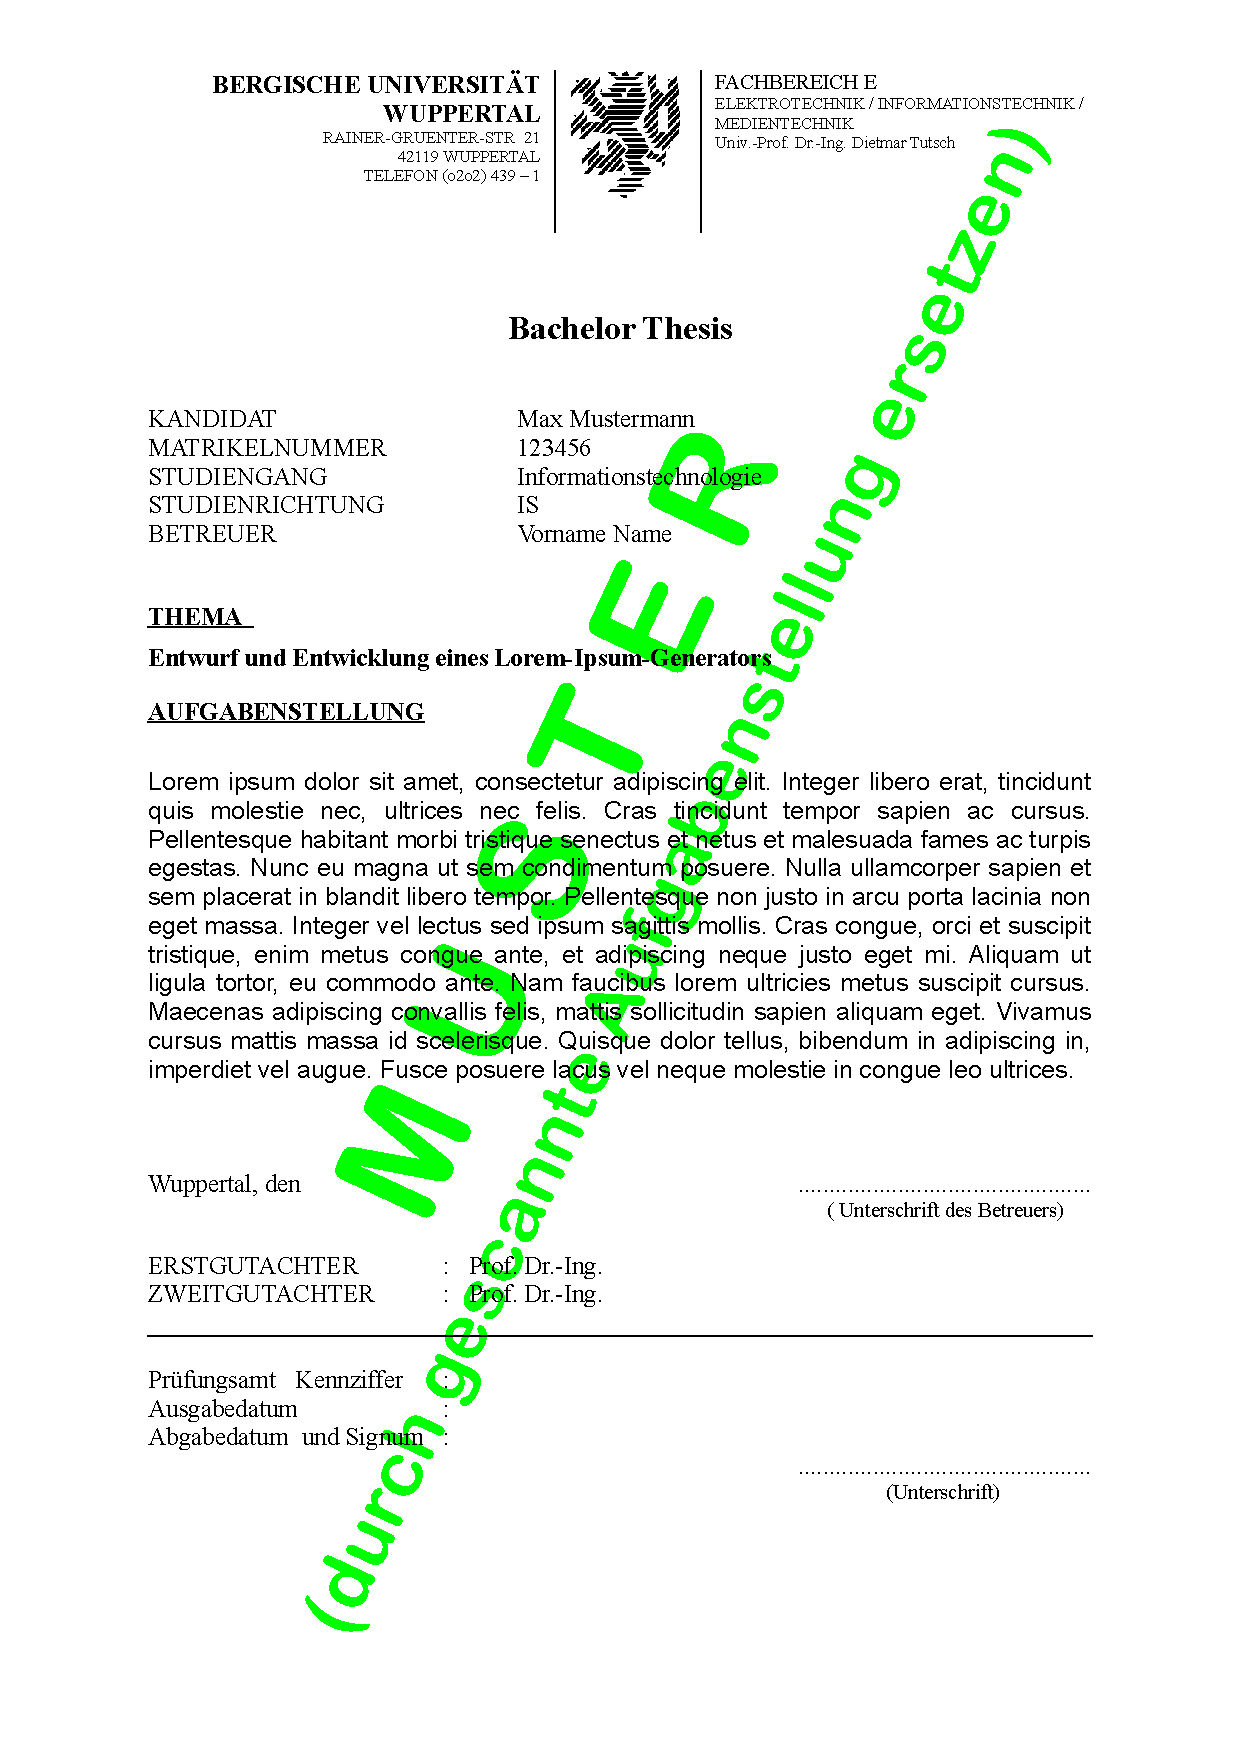
\includepdf[
		%pages={1},
		%fitpaper=true
	%]{Medien/Aufgabenstellung.pdf}%
	%\clearpage{\pagestyle{empty}\cleardoublepage}%
%
%
%%%%%%%%%%%%%%%%%%%%%%%%%%%%%%%%%%%%%%%%%%%%%%%%%%%%%%%%%%%%%%%%%%%%%%%%%%%%%%%%
%%% Verlängerung %%%%%%%%%%%%%%%%%%%%%%%%%%%%%%%%%%%%%%%%%%%%%%%%%%%%%%%%%%%%%%%
%
	%\ifbool{verlaengerung}{%
		%\cleardoublepage%
		%\pdfbookmark[1]{Verlängerung}{verlaengerung}%
		%
\includepdf[pages={1},fitpaper=true]{Medien/Verlaengerung.pdf}%
	  	%\clearpage{\pagestyle{empty}\cleardoublepage}%
	%}{}%
%
%
%%%%%%%%%%%%%%%%%%%%%%%%%%%%%%%%%%%%%%%%%%%%%%%%%%%%%%%%%%%%%%%%%%%%%%%%%%%%%%%%
%%% Erklärungen %%%%%%%%%%%%%%%%%%%%%%%%%%%%%%%%%%%%%%%%%%%%%%%%%%%%%%%%%%%%%%%%
%
	\pdfbookmark[1]{Erklärungen}{erklaerung}%
	\vspace*{2em}%
	
	\vspace*{\fill} % Push content to the vertical center
\begin{center}
    \Huge
    \textbf{If you fail, never give up because FAIL means ``First Attempt in Learning.''}
    
    \vspace{0.5cm}
    \hrule % Horizontal line
    \vspace{0.5cm}
    \large
    (APJ Abdul Kalam)
\end{center}
\vspace*{\fill} % Push content to the vertical center
	\newpage
	\section*{Declaration of Authorship}


\vspace{20pt}

I, Jay Karippacheril Jacob, declare that this thesis titled, "Accelerating the computation of the matrix sign function" and the work presented in it are my own. I confirm that:

\vspace{10pt}

\begin{itemize}
	
	\item This work was been done wholly or mainly while in candidature for a research degree at this University.
	\item Where any part of this thesis has previously been submitted for a degree or any other qualification at this University or any other institution, this has been clearly stated.
	\item Where I have consulted the published work of others, this is always clearly attributed.
	\item Where I have quoted from the work of others, the source is always given. With the exception of such quotations, this thesis is entirely my own	work.
	\item  I have acknowledged all main sources of help.
	\item Where the thesis is based on work done by myself jointly with others, I have made clear exactly what was done by others and what I have contributed myself.
	
\end{itemize}

\vspace{40pt}

\ifbool{zusatzErklaerung}{\vfill}{\vspace{4em}}%
\begin{tabular}{lc}%
	\ort, \abgabedatum \hspace*{1cm}& \rule[2px]{5cm}{0.5px}\\%
	&\footnotesize{(Signature)}%
\end{tabular}
\ifbool{zusatzErklaerung}{\vfill}{\vspace{5em}}%
	
	\newpage
	\section*{Acknowledgment}

First and foremost, I would like to express my heartfelt gratitude to Prof. Dr. Andreas Frommer. From the very first email inquiring about the possibility of working under his supervision to every step throughout the course of this thesis, he has been consistently kind, generous, and supportive. I deeply appreciate his guidance in helping me grasp the critical concepts required for my research and his invaluable assistance in rectifying the mistakes I made along the way. Our weekly meetings were always constructive, enlightening, and filled with engaging discussions, which I truly cherished. It has been a remarkable experience to complete my thesis under his supervision, and I am sincerely grateful for the initial ideas and references he provided that shaped the foundation of this work.

\vspace{10pt}

I am also deeply grateful to Dr. Gustavo Alonso Ramirez Hidalgo for his exceptional support and guidance. At the early stages of my thesis, I found certain technical concepts challenging to understand, but his clear explanations helped me navigate through these difficulties. I greatly appreciate the time and effort he invested in reviewing my algorithms and code, ensuring better implementations. Despite leaving the University of Wuppertal, he continued to offer his support, for which I will always be indebted. 

\vspace{10pt}

I would also like to extend my gratitude to Jose Jimenez Merchan for stepping in during the final stages of my thesis and offering guidance to me.

\vspace{10pt}

To Prof. Dr. Andreas Frommer, Dr. Gustavo Alonso Ramirez Hidalgo, and José Jiménez Merchán, I am immensely thankful for their unique personalities, unwavering support, and the time they dedicated to me throughout my master's thesis journey.

\vspace{10pt}

Lastly, I would like to express my heartfelt appreciation to my family, friends, and the Faculty of Mathematics and Natural Sciences at the University of Wuppertal. Their constant encouragement, support, and belief in me have been a source of strength throughout my master’s journey.

\vspace{20pt}

Thank you all for being an integral part of this significant milestone in my life.

	\newpage
	\section*{Abstract}

The matrix sign function arises in computations in lattice QCD. We look at the computation of the action $\text{sign}(Q)x$ of the sign function of the matrix $Q$ on a vector $x$. In our application, $Q$ is the symmetrized Wilson-Dirac operator. This is a Hermitian matrix if the chemical potential is 0; otherwise, it is non-Hermitian. Actually, we will always consider the inverse square root function, since $\text{sign}(Q)x = (Q^2)^{-1/2}Qx$.

The Arnoldi Krylov subspace approximation is the basis method to approximate $\text{sign}(Q)x$. There are several ways to accelerate the convergence of this basic scheme:
\begin{enumerate}
    \item \textbf{Restarts} (in the non-Hermitian case). This avoids having too many inner products in the Arnoldi orthogonalization.
    \item \textbf{Deflation} (explicit and implicit). This makes the matrix better conditioned and thus reduces the number of iterations. Explicit deflation uses the smallest left and right eigenvectors; implicit deflation is present in the thick restart approach of Eiermann and Güttel; see also the \texttt{funm} Matlab code.
    \item \textbf{Polynomial preconditioning.} This also makes the matrix better conditioned and thus reduces the number of iterations. A recent paper on this was published along with the numerical results for QCD on a parallel machine.
    \item \textbf{Sketching.} This is a randomized approach where we save orthogonalizations and sketch the Arnoldi matrix. The relevant paper is by Güttel and Schweitzer.
\end{enumerate}

\textbf{The purpose of the thesis} is to consider the following combination of the above approaches:
\begin{itemize}
    \item $2 + 1$ (as is already done in \texttt{funm})
    \item $2 + 3$ (building on existing work and code of Gustavo)
    \item $2 + 4$ (this is new, but Stefan Güttel just gave a talk on it at a conference in Paris)
\end{itemize}

\textbf{Tasks:}
\begin{enumerate}
    \item Understand and describe the individual methods (1--4).
    \item Describe, formulate algorithmically, and discuss the combined methods ($2+1$, $2+3$, $2+4$).
    \item Test the combined methods, in Matlab on small configurations.
\end{enumerate}





%
%
%%%%%%%%%%%%%%%%%%%%%%%%%%%%%%%%%%%%%%%%%%%%%%%%%%%%%%%%%%%%%%%%%%%%%%%%%%%%%%%%
%%% Danksagung %%%%%%%%%%%%%%%%%%%%%%%%%%%%%%%%%%%%%%%%%%%%%%%%%%%%%%%%%%%%%%%%%
	%\ifbool{danksagung}{%
		%\vspace*{\fill}\vspace{-3em}%
		%\pdfbookmark[1]{Danksagung}{danksagung}%
		%\section*{Danksagung}
\todo{Text der Danksagung wird hier eingetragen.}

Lorem ipsum dolor sit amet, consectetur adipiscing elit. Integer libero erat, tincidunt quis molestie nec, ultrices nec felis. Cras tincidunt tempor sapien ac cursus. Pellentesque habitant morbi tristique senectus et netus et malesuada fames ac turpis egestas. Nunc eu magna ut sem condimentum posuere. Nulla ullamcorper sapien et sem placerat in blandit libero tempor. Pellentesque non justo in arcu porta lacinia non eget massa. Integer vel lectus sed ipsum sagittis mollis. Cras congue, orci et suscipit tristique, enim metus congue ante, et adipiscing neque justo eget mi. Aliquam ut ligula tortor, eu commodo ante. Nam faucibus lorem ultricies metus suscipit cursus. Maecenas adipiscing convallis felis, mattis sollicitudin sapien aliquam eget. Vivamus cursus mattis massa id scelerisque. Quisque dolor tellus, bibendum in adipiscing in, imperdiet vel augue. Fusce posuere lacus vel neque molestie in congue leo ultrices.%
		%\vfill%
	%}{}
%
%
%%%%%%%%%%%%%%%%%%%%%%%%%%%%%%%%%%%%%%%%%%%%%%%%%%%%%%%%%%%%%%%%%%%%%%%%%%%%%%%%
%%% Kurzfassung & Abstract %%%%%%%%%%%%%%%%%%%%%%%%%%%%%%%%%%%%%%%%%%%%%%%%%%%%%
%
	%\clearpage{\pagestyle{empty}\cleardoublepage}
	%\vspace*{\fill}\vspace{-3em}
	%\pdfbookmark[1]{Kurzfassung}{kurzfassung}
	%%% Version 2023-08-21
%% LaTeX-Vorlage für Abschlussarbeiten
%% Erstellt von Nils Potthoff, ab 2020 erneuert und ausgebaut von Simon Lohmann
%% Lehrstuhl Automatisierungstechnik/Informatik Bergische Universität Wuppertal
%%%%%%%%%%%%%%%%%%%%%%%%%%%%%%%%%%%%%%%%%%%%%%%%%%%%%%%%%%%%%%%%%%%%%%%%%%%%%%%%

% INFO: Die Kurzfassung wird immer auf Deutsch UND Englisch benötigt!

% Kurzfassung auf Deutsch
\begingroup 
	\selectlanguage{ngerman}% der folgende Text ist auf Deutsch
	\section*{Kurzfassung}
	\todo{Der Text der Kurzfassung wird hier eingetragen.}
	\blindtext
\endgroup

% Kurzfassung auf Englisch
\begingroup
	\selectlanguage{english}% der folgende Text ist auf Englisch
	\section*{Abstract}
	\todo{The english version.}
	\blindtext
\endgroup

	\vfill
	\clearpage
%
%
%%%%%%%%%%%%%%%%%%%%%%%%%%%%%%%%%%%%%%%%%%%%%%%%%%%%%%%%%%%%%
%  INHALTSVERZEICHNIS
\markboth{\contentsname}{}
\pdfbookmark[1]{\contentsname}{toc}
\begingroup
	\renewcommand{\markboth}[2]{}{}
	\tableofcontents
\endgroup
\clearpage
%
%
%%WIDMUNG, VORWORT
%
%% Ende der Titelei; es folgt der Hauptteil
\ifbool{doppelseitig}{%
	\clearpage%
	\hphantom{anker, damit hier auch wirklich eine leere Seite ist}%
}{}%
{\pagestyle{empty}\cleardoublepage}% Inhalt soll auf rechter Seite beginnen
\pagenumbering{arabic}%
\pagestyle{thesis-page-regular}%

 % Titelseite etc. (bitte nicht ändern) %%%%%%%%%
	%%%%%%%%%%%%%%%%%%%%%%%%%%%%%%%%%%%%%%%%%%%%%%%%%%%%%%%%%%%%%%%%%%%%%%%%%%%%
	%%%%%%%%%%%%%  Ab hier ändern und ergänzen  %%%%%%%%%%%%%%%%%%%%%%%%%%%%%%%%
	%%%%%%%%%%%%%  | | | | | | | | | | | | | |  %%%%%%%%%%%%%%%%%%%%%%%%%%%%%%%%   
	%%%%%%%%%%%%%  V V V V V V V V V V V V V V  %%%%%%%%%%%%%%%%%%%%%%%%%%%%%%%%
	
	% weitere .tex-Dateien werden mit \input eingebunden
	% (z.B. eine für jedes Kapitel)

	% Einführungskapitel
	\chapter{Einleitung}

	{
		\todo[inline]{%
			Im Anhang dieses Dokuments gibt es die Kapitel \nameref{sec:anhang:faq} und \nameref{sec:anhang:latex-beispiele},\\die euch bei Problemen oder Fragen zu LaTeX und der Thesisvorlage helfen können.
		}
	}
	
	\section{Motivation}
		\todo[inline]{%
			Hier soll das Thema motiviert werden.
			Bitte nicht \enquote{Ich bin besonders motiviert, weil ...}
			sondern \enquote{Thema/Projekt XY ist wichtig/muss untersucht/soll entwickelt werden, weil ...}
		} 
		\blindtext
		
	\section{Problemstellung \& Ziele}
		\todo[inline]{%
			Hier sollen die Problemstellung und das Ziel der Thesis kurz in eigenen Worte erläutert werden.
		}
		\blindtext
		
		
	\section{Aufbau der Thesis}
		\todo[inline]{%
			Überblick über den Aufbau der Thesis. Welche Kapitel behandeln was?
		}
		\blindtext
		
		
	\section{Notation}
		\todo[inline]{%
			(optional)\\
			Wenn in der Thesis eine besondere Notation eingeführt/verwendet wird, ist diese hier kurz zu erklären. Andernfalls kann dieser Abschnitt entfallen.
		}
		\blindtext
	%% Version 2023-08-21
%% LaTeX-Vorlage für Abschlussarbeiten
%% Erstellt von Nils Potthoff, ab 2020 erneuert und ausgebaut von Simon Lohmann
%% Lehrstuhl Automatisierungstechnik/Informatik Bergische Universität Wuppertal
%%%%%%%%%%%%%%%%%%%%%%%%%%%%%%%%%%%%%%%%%%%%%%%%%%%%%%%%%%%%%%%%%%%%%%%%%%%%%%%%

\chapter{Grundlagen}
	\todo[inline]{%
		Hier werden die Grundlagen der Thematik erklärt.
		Das können z.B. mathematische Grundlagen, Kommunikationsprotokolle oder spezielle Algorithmen sein.\\
		Übliches Wissen aus unserer Fakultät wie z.B. die Formel $U = R*I$ oder die Funktionsweise von Schleifen und Arrays kann vorausgesetzt werden.
		\\~\\
		Faustregel: alles, was man selber vorher nicht wusste, aber auch nicht selber entwickelt hat.
		\\~\\
		Hier gilt es aber auch auf Erst- und Zweitgutachter einzugehen.
		Wenn man weiß, dass einer der beiden ein Thema nicht so genau kennt, sollte es evtl. doch in die Grundlagen.
		\\~\\
		=> im Zweifelsfall den Betreuer fragen
	}
	
	\section{Verwendete Protokolle}
		\subsection[I³C]{I³C (Inter-Integrated IC Circuit)}
			\blindtext
		\subsection{\texorpdfstring{B$^\text{U}_\text{W}$ 4.0}{BUW 4.0}}
			\blindtext
		\subsection[HTML]{HTML (berühmtes Internetprotokoll)}
			\blindtext
		
		
	\section{Elektrotechnik}
		\subsection{Richtungsabhängigkeit von passiven Bauteilen}
			\blindtext
		\subsection{Neulingsche \glqq Geht ohne Kondensator\grqq-Vermutung}
			\blindtext
		\subsection{Liquid Crystal LCD-Displays}
			\blindtext
		
	\section{Mathematik}
		\subsection{Numerische Evaluation der Division durch Null}
			\blindtext
		\subsection{Die ganzverwurschtelte Invers-Transformation}
			\blindtext
		\subsection{V\o{}\v{r}w\ae{}r\v{s}\'{e} \c{K}\"{\i}\~{n}\k{e}m\aa{}\c{t}i\c{k}}
			\blindtext
		
	\section{Wirtschaft}
		\subsection{Die Erwerbsregeln der Ferengi-Allianz}
			\blindtext
			
		\subsection{Toilettenpapier -- Krisensichere Geldanlage?}
			\blindtext
			
		\subsection{Kostenevaluation ausführlich schwafelnder und aus dem soeben genannten Grunde völlig übertrieben langer Abschnittsüberschriften in Textdokumenten}
			\blindtext
			
%\chapter{Dies ist ein sehr langer Kapitelname, der daher in der bisherigen Vorlage zu gewissen Problemen mit überlappendem Text in der Kopfzeile einer Seite führen konnte}
%	\blindtext
%	\clearpage
%	\blindtext
%	\section{Kostenevaluation ausführlich schwafelnder und aus dem soeben genannten Grunde völlig übertrieben langer Abschnittsüberschriften in Textdokumenten}
%	\clearpage
%	\blindtext

		

	
	
	% weitere (eigene) Kapitel
	\chapter{Entwurf}
	\section{title}
		\subsection{title}
			\blindtext

			\blindtext
			\blindtext
			
			\blindtext
			\blindtext
		\subsection{title}
		
			\blindtext
	
	\section{title}
		\subsection{title}
			\blindtext
		
			\blindtext
		\subsection{title}
			\blindtext
		

	%% Version 2023-08-21
%% LaTeX-Vorlage für Abschlussarbeiten
%% Erstellt von Nils Potthoff, ab 2020 erneuert und ausgebaut von Simon Lohmann
%% Lehrstuhl Automatisierungstechnik/Informatik Bergische Universität Wuppertal
%%%%%%%%%%%%%%%%%%%%%%%%%%%%%%%%%%%%%%%%%%%%%%%%%%%%%%%%%%%%%%%%%%%%%%%%%%%%%%%%

\chapter{Realisierung}
	\section{title}
		\blindtext
		
		\blindtext
		\blindtext
		
	\section{title}
		\blindtext
		
		\blindtext
		
		\blindtext

		\subsection{title}
			\blindtext
			
			\blindtext
		\subsection{title}
			\blindtext
		
			
			
			\begin{figure}
				\centering
				\begin{tikzpicture}
				\duck[speech={\small Quaak!}, bubblecolor=cyan!20!white, laughing]
				\end{tikzpicture}
				\caption{Bildbeschreibungen sind wichtig, damit der Leser versteht, was er da sieht. Allerdings sollten sie nicht unnötig lang sein -- längere Texte, wie zum Beispiel dieser hier, der ausführlich erläutert, dass auf dem Bild eine gelbe Ente zu sehen ist, welche den Schnabel geöffnet hat und \enquote{Quaak!} sagt, gehören in den normalen Fließtext.}
			\end{figure}

	%...

	% Schlusskapitel
	%% Version 2023-08-21
%% LaTeX-Vorlage für Abschlussarbeiten
%% Erstellt von Nils Potthoff, ab 2020 erneuert und ausgebaut von Simon Lohmann
%% Lehrstuhl Automatisierungstechnik/Informatik Bergische Universität Wuppertal
%%%%%%%%%%%%%%%%%%%%%%%%%%%%%%%%%%%%%%%%%%%%%%%%%%%%%%%%%%%%%%%%%%%%%%%%%%%%%%%%

\chapter{Analyse}
	\todo[inline]{%
		In diesem Kapitel analysiert ihr eure Ergebnisse.
		\\\medskip
		Was funktioniert wie gewünscht?\\
		Was funktioniert noch nicht (oder noch nicht ganz richtig)?\\
		~~~~-> kann man dann auch im Ausblick erwähnen\\\medskip
		Wichtig: Wie gut sind die Ergebnisse (z.B. Fehlerrate, Genauigkeit, Wiederholbarkeit, ...)\\
		\bigskip
		\textbf{In der Analyse schreibt man eine wissenschaftliche Auswertung, keine persönliche Meinung!} (die kommt ggf. im Fazit)\\
		\bigskip
		Wenn etwas nicht gut funktioniert, sollte hier eine Fehleranalyse stehen. Selbst wenn man den Fehler vielleicht nicht komplett lösen konnte, kann man so zeigen, dass man systematisch nach einer Lösung gesucht hat (Unter welchen Bedingungen tritt das Problem auf? Regelmäßig oder Unvorhersehbar? Gibt es sonstige Auffälligkeiten? etc.).
	}
	
	\section{title}
	\blindtext
	
	\section{title}
	\blindtext

	\chapter{Schlussbetrachtungen}
	\todo[inline]{Hier ist wieder eigene Meinung erlaubt}
	\section{Fazit}
		\todo[inline]{Was wurde erreicht? Was fehlt oder ist nicht fertig geworden? Wurde irgendetwas über die Aufgabenstellung hinausgehendes gemacht?}
		\blindtext
	\section{Ausblick}
		\todo[inline]{Wie könnte man an dem Projekt weiterarbeiten? Dieser Abschnitt ist eine gute Gelegenheit noch offene Baustellen anzusprechen und ggf. kurze Vorschläge dazu zu machen}
		\blindtext

	%%%%%%%%%%%%%%%%%%%%%%%%%%%%%%%%%%%%%%%%%%%%%%%%%%%%%%%%%%%%%%%%%%%%%%%%%%%%
	\appendix % Ende des Inhalts, hier beginnt der Anhang %%%%%%%%%%%%%%%%%%%%%%
	%%%%%%%%%%%%%%%%%%%%%%%%%%%%%%%%%%%%%%%%%%%%%%%%%%%%%%%%%%%%%%%%%%%%%%%%%%%%
	%%%%%%%%%%%%%%%%%%%%%%%%%%%%%%%%%%%%%%%%%%%%%
%%% ! WARNUNG ! %%%%%%%%%%%%%%%%%%%%%%%%%%%%%
%%%%%%%%%%%%%%%%%%%%%%%%%%%%%%%%%%%%%%%%%%%%%
%%%  Diese Datei bitte nur bearbeiten,    %%%
%%%   wenn du ein LaTeX-Experte bist      %%%
%%%             U N D                     %%%
%%%  die Vorlage unbedingt ändern willst  %%%
%%%%%%%%%%%%%%%%%%%%%%%%%%%%%%%%%%%%%%%%%%%%%
%%%%%%%%%%%%%%%%%%%%%%%%%%%%%%%%%%%%%%%%%%%%%
%
%%%%%%%%%%%%%%%%%%%%%%%%%%%%%%%%%%%%%%%%%%%%%%%%%%%%%%%%%%%%%%%%%%%%%%%%%%%%%%%%
%%% DATEI-INFO %%%%%%%%%%%%%%%%%%%%%%%%%%%%%%%%%%%%%%%%%%%%%%%%%%%%%%%%%%%%%%%%%
%%%%%%%%%%%%%%%%%%%%%%%%%%%%%%%%%%%%%%%%%%%%%%%%%%%%%%%%%%%%%%%%%%%%%%%%%%%%%%%%
%%% Diese Datei generiert diverse Verzeichnisse %%%%%%%%%%%%%%%%%%%%%%%%%%%%%%%%
%%%%%%%%%%%%%%%%%%%%%%%%%%%%%%%%%%%%%%%%%%%%%%%%%%%%%%%%%%%%%%%%%%%%%%%%%%%%%%%%
%
%SONSTIGE VERZEICHNISSE
\clearpage{\pagestyle{empty}\cleardoublepage}%
\begingroup
	% Lokaler Override -> Verzeichnisse tragen sich gerne mal sowohl als aktuelles Kapitel als auch aktuelles Unterkapitel ein - dass steht in der Kopfzeile dann doppelt da und sieht hässlich aus!
	\let\oldmarkboth\markboth
	\renewcommand{\markboth}[2]{
		\oldmarkboth{#1}{}
	}
	
	
	\ifbool{verzeichnisseZusammenfassen}{% Seitenumbruch durch Abstand ersetzen, wenn gewünscht
		\def\clearpage{\vspace{2em}}%
	}{}%
%
%
	\ifbool{abbildungsverzeichnis}{%
		\clearpage%
		\verzeichnisEintrag{\listfigurename}{lof}
		\setlength{\cftfigindent}{0em}% Verzeichniseinträge ohne extra Indent darstellen
		\listoffigures%
	}{}%
%
%
	%\ifbool{quellcodeverzeichnis}{%
		%\clearpage%
		%\verzeichnisEintrag{\lstlistlistingname}{listings}
		% indent wird in Präambel entfernt
		%\lstlistoflistings%
	%}{}%
%
%
\clearpage
	\ifbool{tabellenverzeichnis}{%
		\clearpage%
		\verzeichnisEintrag{\listtablename}{lot}
		\setlength{\cfttabindent}{0em}% Verzeichniseinträge ohne extra Indent darstellen
		\listoftables%
	}{}%
%
	
%		\clearpage%
%		%Redefinition des Stils von "siehe {anderer Begriff}":
%		\renewcommand\glsseeformat[3][\seename]{%
%			\\*% non breaking new line
%			\emph{#1} \glsseelist{#2}%
%		}
%
		% Anwendbare Styles (es gibt noch viel mehr): 
		% mcolist 			: mehrspaltig
		% mcolindexgroup 	: spalten+Anfangsbuchstaben über Gruppen
		% altlist			: 		
		% long				:
		%
		% nogroupskip deaktiviert den Abstand zwischen Gruppen (CLK und CRC gehören zu einer Gruppe, weil sie beide mit C beginnen)
	\ifbool{symbolverzeichnis}{%
		\vspace{-1em}
		\setlength{\glsdescwidth}{.75\linewidth}
		% TODO: Verzeichnisbreite dynamisch anpassen, z.B. mit https://tex.stackexchange.com/questions/174652/glossaries-package-how-to-format-the-positions-of-the-columns-and-width-of-the
		\verzeichnisEintrag{\glssymbolsgroupname}{listofsymbols}
		\printnoidxglossary[type=symbols,		style=altlongragged4col,nogroupskip]
		\vspace{-1em}
	}{}%
	
%	\verzeichnisEintrag{Irgendeinverzeichnis}{label-fuer-irgendeinverzeichnis}
%	
%	\chapter*{Irgendeinverzeichnis}
%		\begin{tabular}{ll}
%		$a$ & 124\\
%		$b_e$ & 2\\
%		$\phi_+^\sigma$ & $\frac{61}{9}$\\
%		$d$ & 42
%		\end{tabular}
	
	\ifbool{abkuerzungsverzeichnis}{%
%		\setlength{\glsdescwidth}{.85\linewidth}
		% TODO: Verzeichnisbreite dynamisch anpassen, z.B. mit https://tex.stackexchange.com/questions/174652/glossaries-package-how-to-format-the-positions-of-the-columns-and-width-of-the
		\SaveTranslation{\abbreviationsnamesaved}{abbreviationsname}
		\verzeichnisEintragX{\GetTranslation{abbreviationsname}}{\abbreviationsnamesaved}{listofabbreviations}
		\printnoidxglossary[type=abbreviations,	style=longragged3col,nogroupskip, title={\GetTranslation{abbreviationsname}}]
		\vspace{-1em}
	}{}%
	\ifbool{akronymverzeichnis}{%
		\verzeichnisEintrag{\acronymname}{listofacronyms}
		\printnoidxglossary[type=acronym,		style=mcolindex,nogroupskip]
		\vspace{-1em}
	}{}%
	%\ifbool{glossar}{%
		%\verzeichnisEintrag{\glossaryname}{glossary}
		%\printnoidxglossary[type=main,			style=altlist,nogroupskip]
%		\par
	%}{}%
	%	
	%%Literaturverzeichnis
	\ifbool{weiterfuehrendeLiteratur}{%
		\verzeichnisEintrag{\GetTranslation{Bibliography}}{literature}
		\printbibliography[title={\GetTranslation{Bibliography}},category=cited]%
		
		%\SaveTranslation{\furtherreadingsaved}{FurtherReading}% Umweg, da ggf. Umlaute enthalten sind und das sonst direkt nicht klappt
		%\verzeichnisEintragX{\GetTranslation{FurtherReading}}{\furtherreadingsaved}{furtherreading}
		\printbibliography[title={\GetTranslation{FurtherReading}},notcategory=cited]%
	}{%
		\verzeichnisEintrag{\GetTranslation{Bibliography}}{literature}
		\printbibliography[title={\GetTranslation{Bibliography}}]%
	}%
%
\endgroup% Verzeichnisse (bitte nicht ändern) %%%%%%%%%%%%%
	%%%%%%%%%%%%%%%%%%%%%%%%%%%%%%%%%%%%%%%%%%%%%%%%%%%%%%%%%%%%%%%%%%%%%%%%%%%%
	
	% Anhänge
%	\input{Kapitel/Klassendiagramm}
%	\input{Kapitel/Versuchsaufbauten}
%	%% Version 2023-08-21
%% LaTeX-Vorlage für Abschlussarbeiten
%% Erstellt von Nils Potthoff, ab 2020 erneuert und ausgebaut von Simon Lohmann
%% Lehrstuhl Automatisierungstechnik/Informatik Bergische Universität Wuppertal
%%%%%%%%%%%%%%%%%%%%%%%%%%%%%%%%%%%%%%%%%%%%%%%%%%%%%%%%%%%%%%%%%%%%%%%%%%%%%%%%

\chapter{Schaltpläne}
	\section{Schaltplan}
		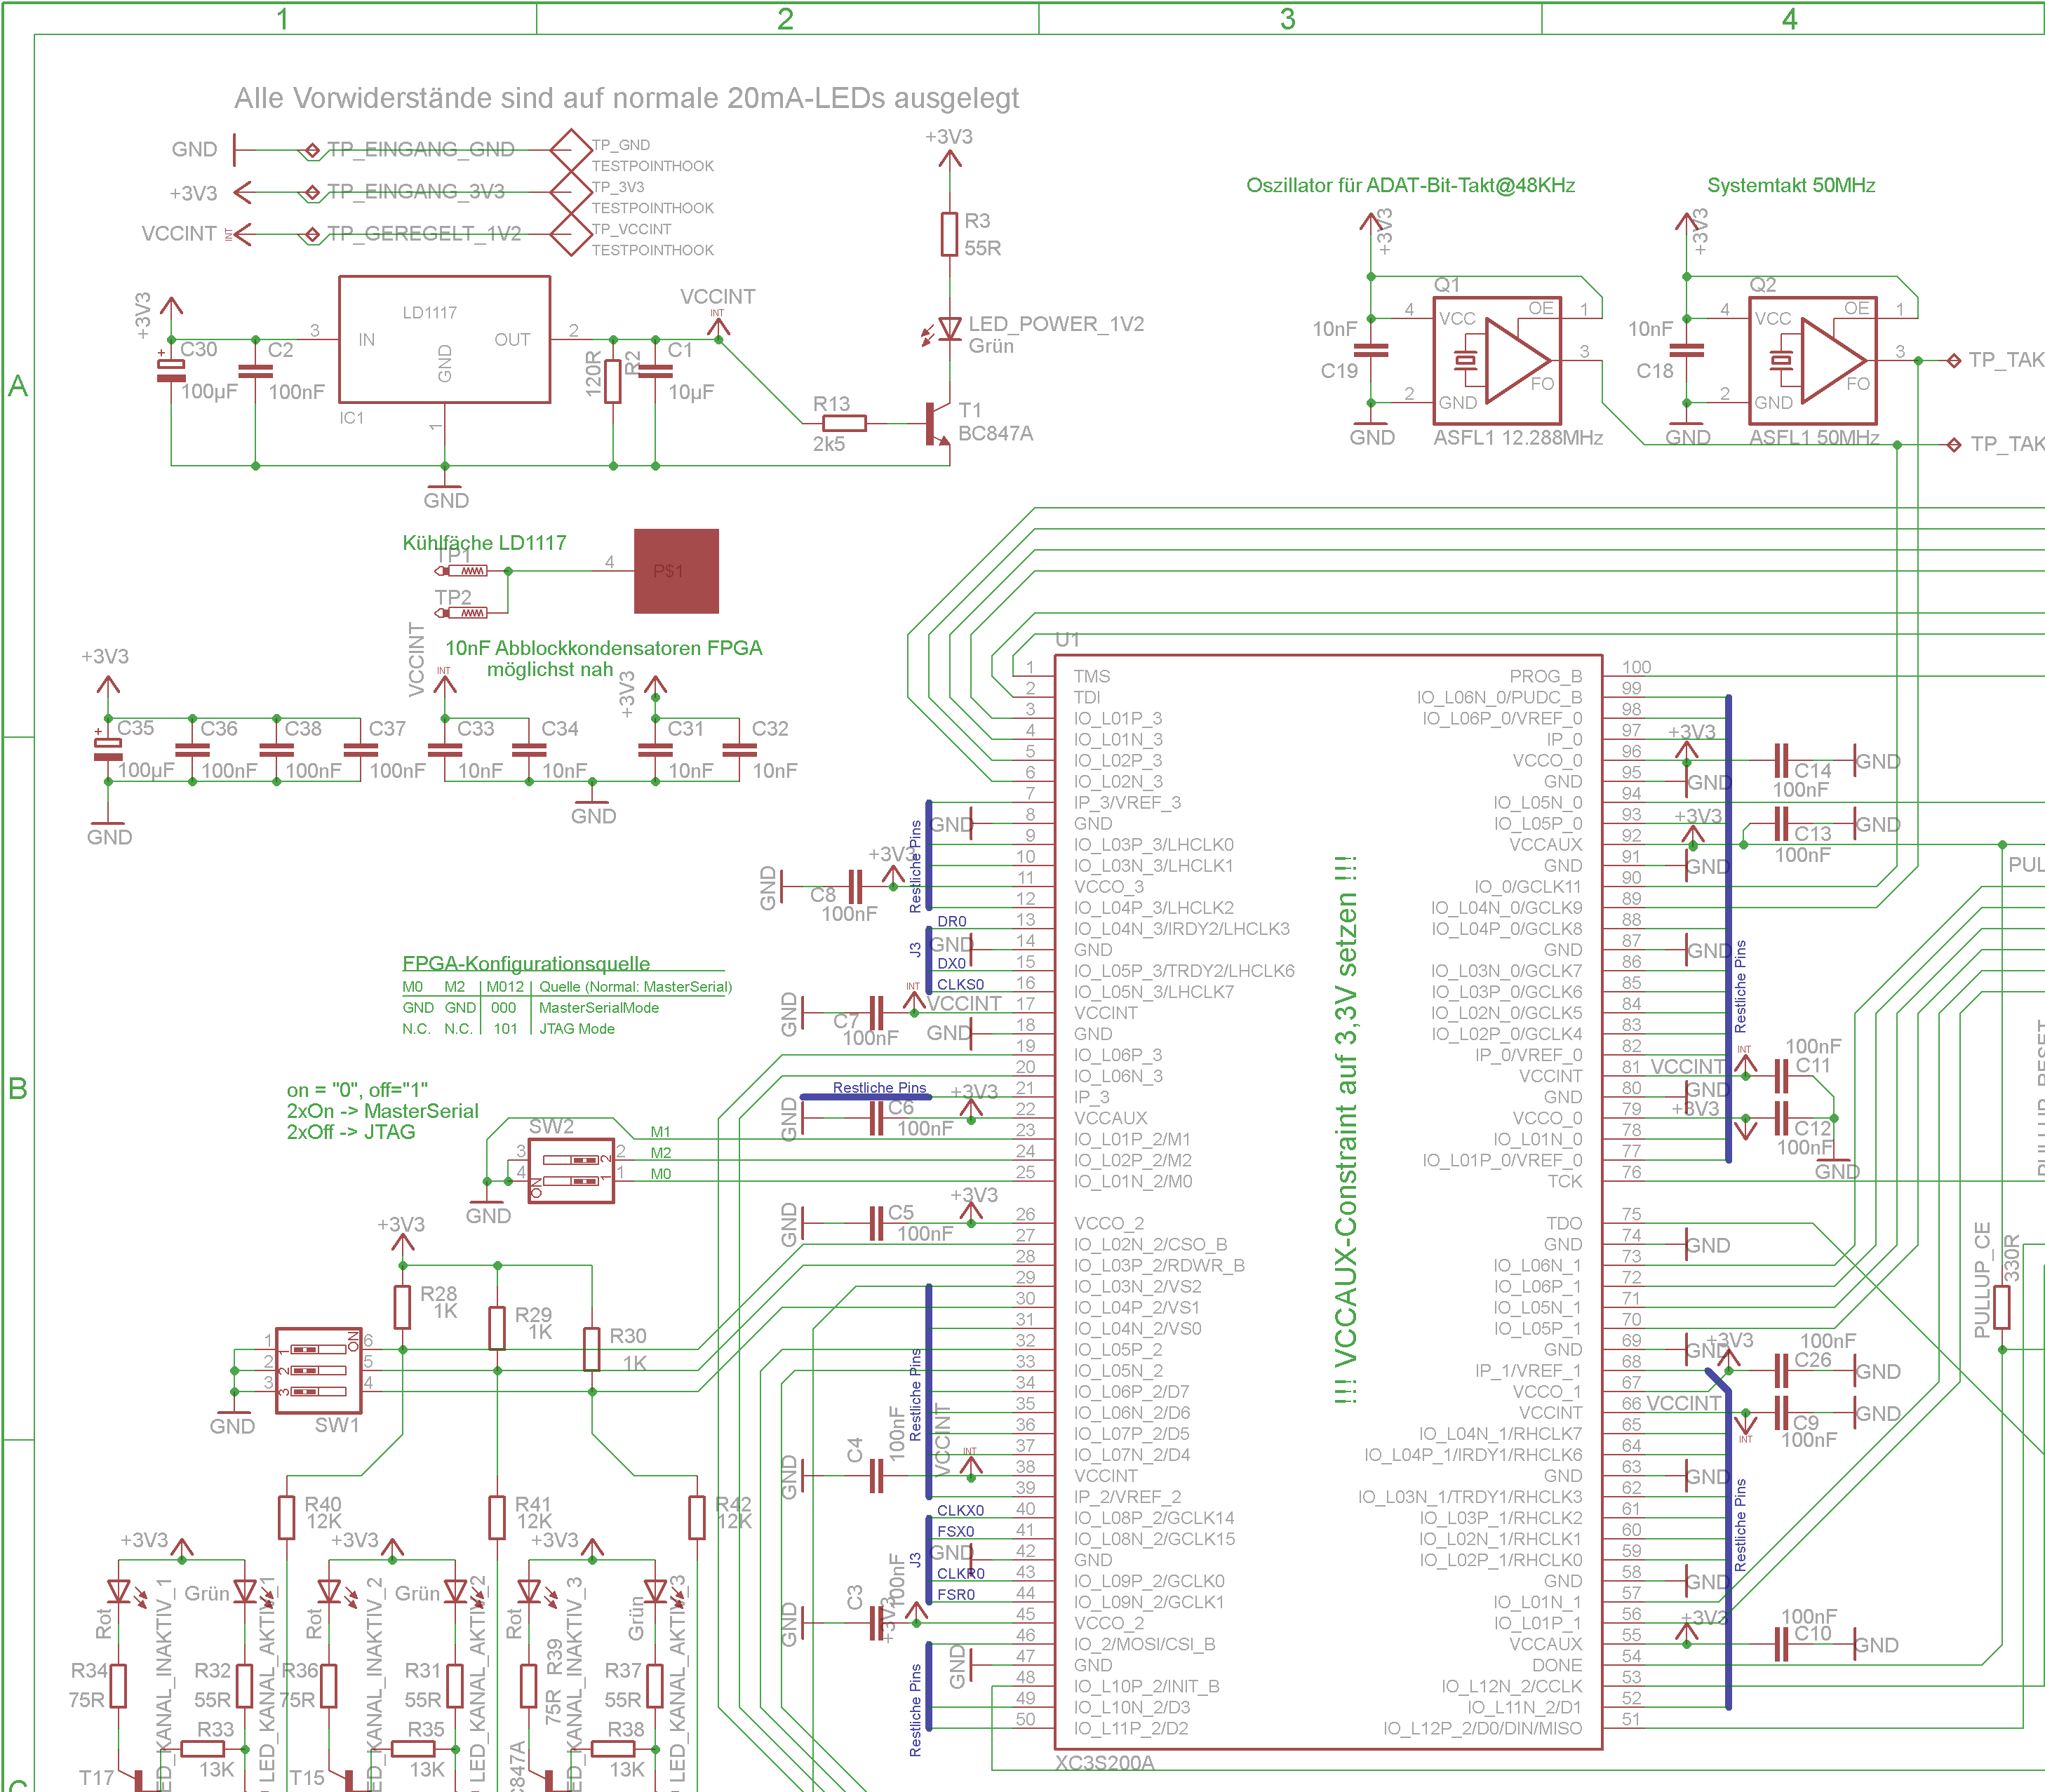
\includegraphics[width=\linewidth]{Medien/schaltplan1.png}
		\clearpage
		
		\noindent
		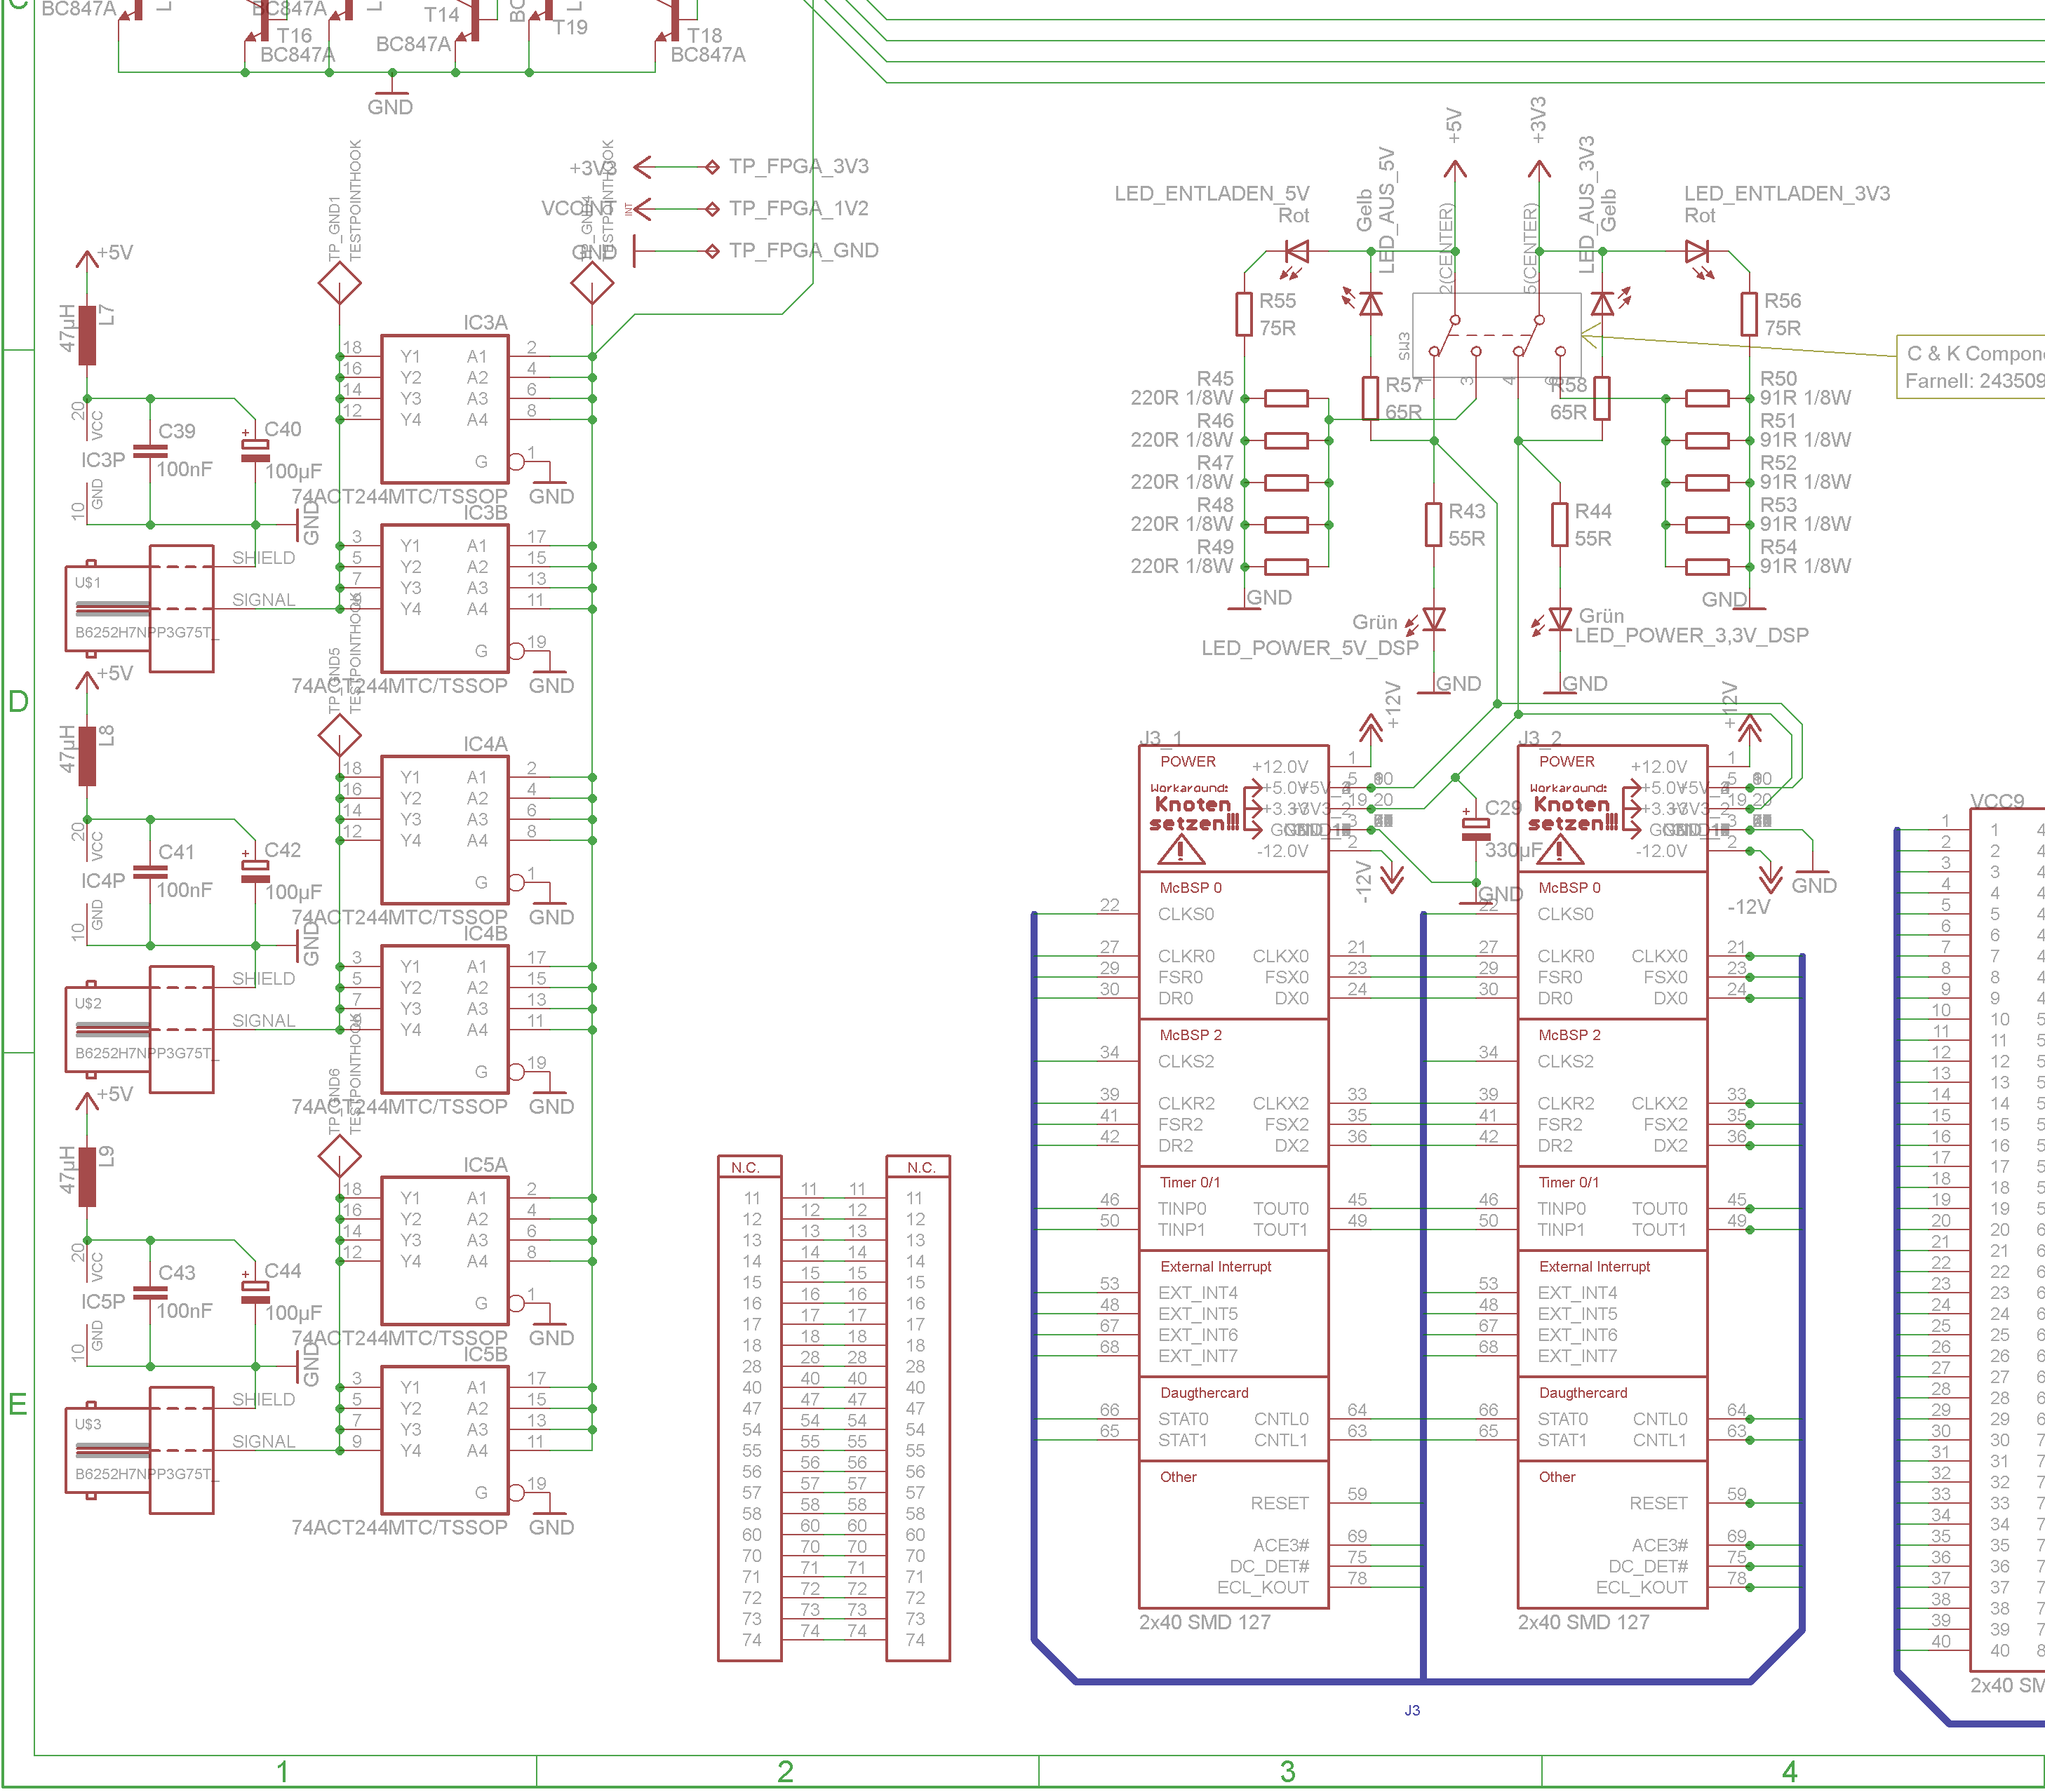
\includegraphics[width=\linewidth]{Medien/schaltplan2.png}
		\clearpage
		 
		\noindent
		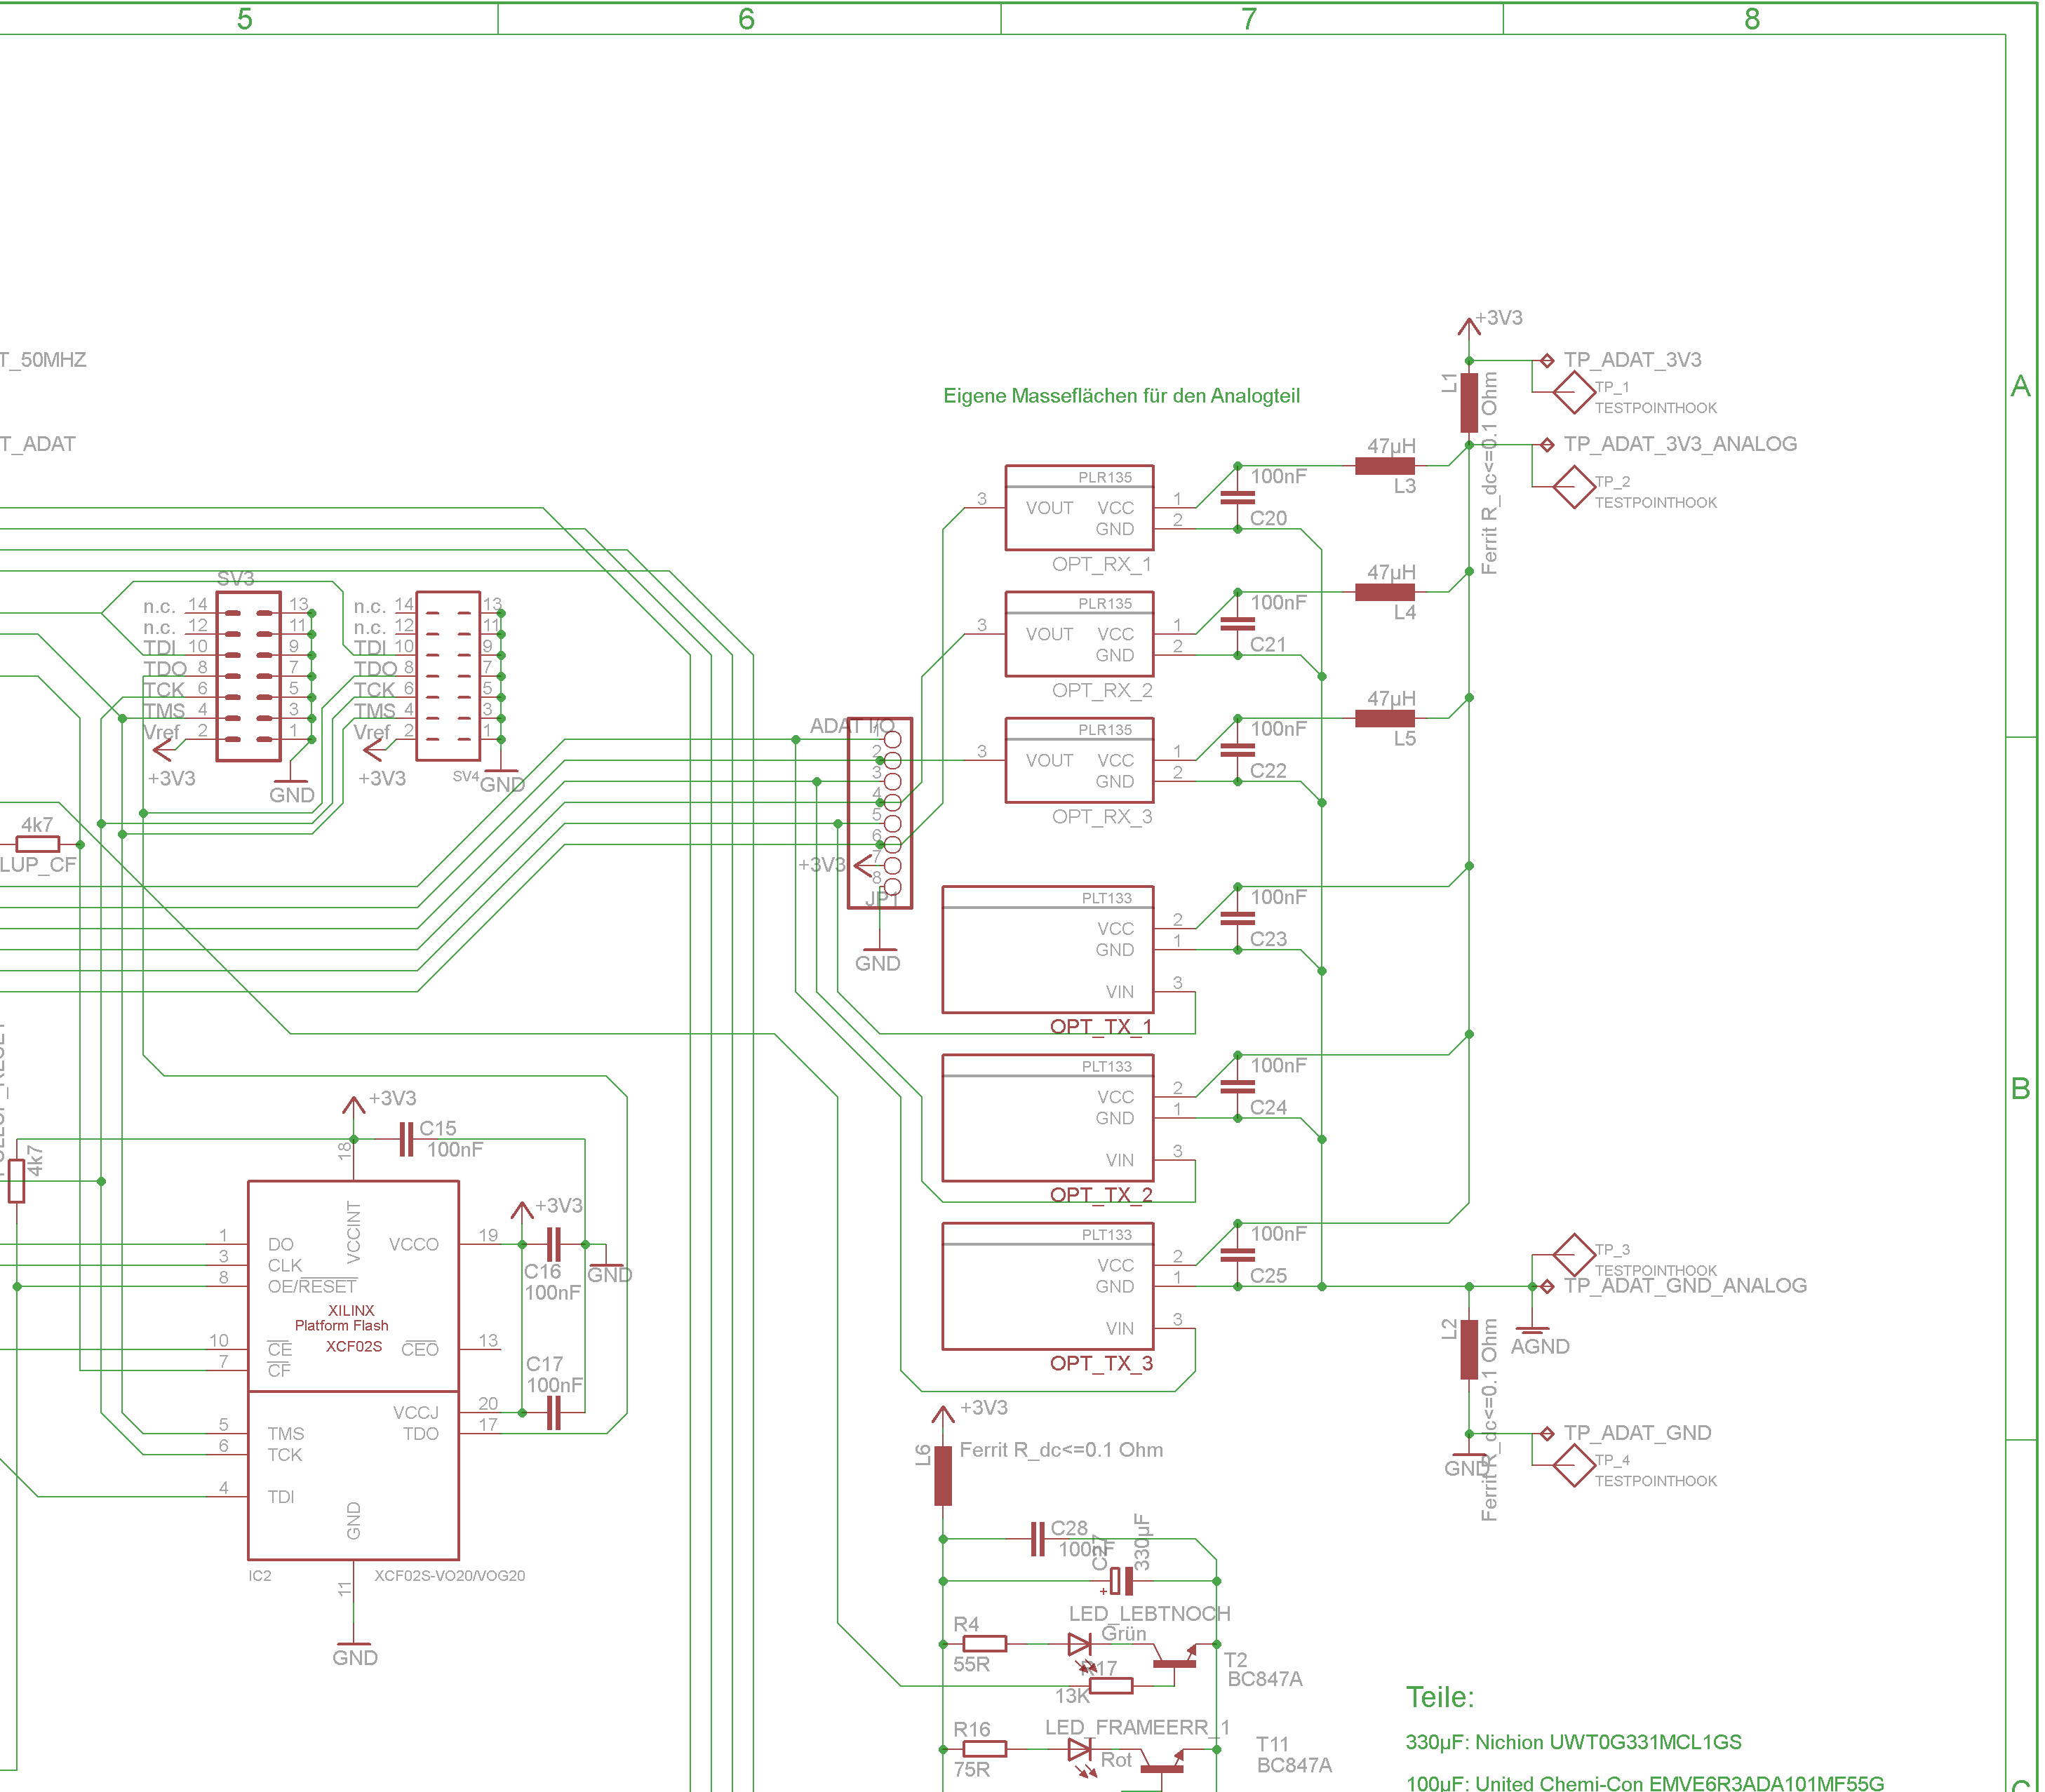
\includegraphics[width=\linewidth]{Medien/schaltplan3.png}
		\clearpage
		
		\noindent
		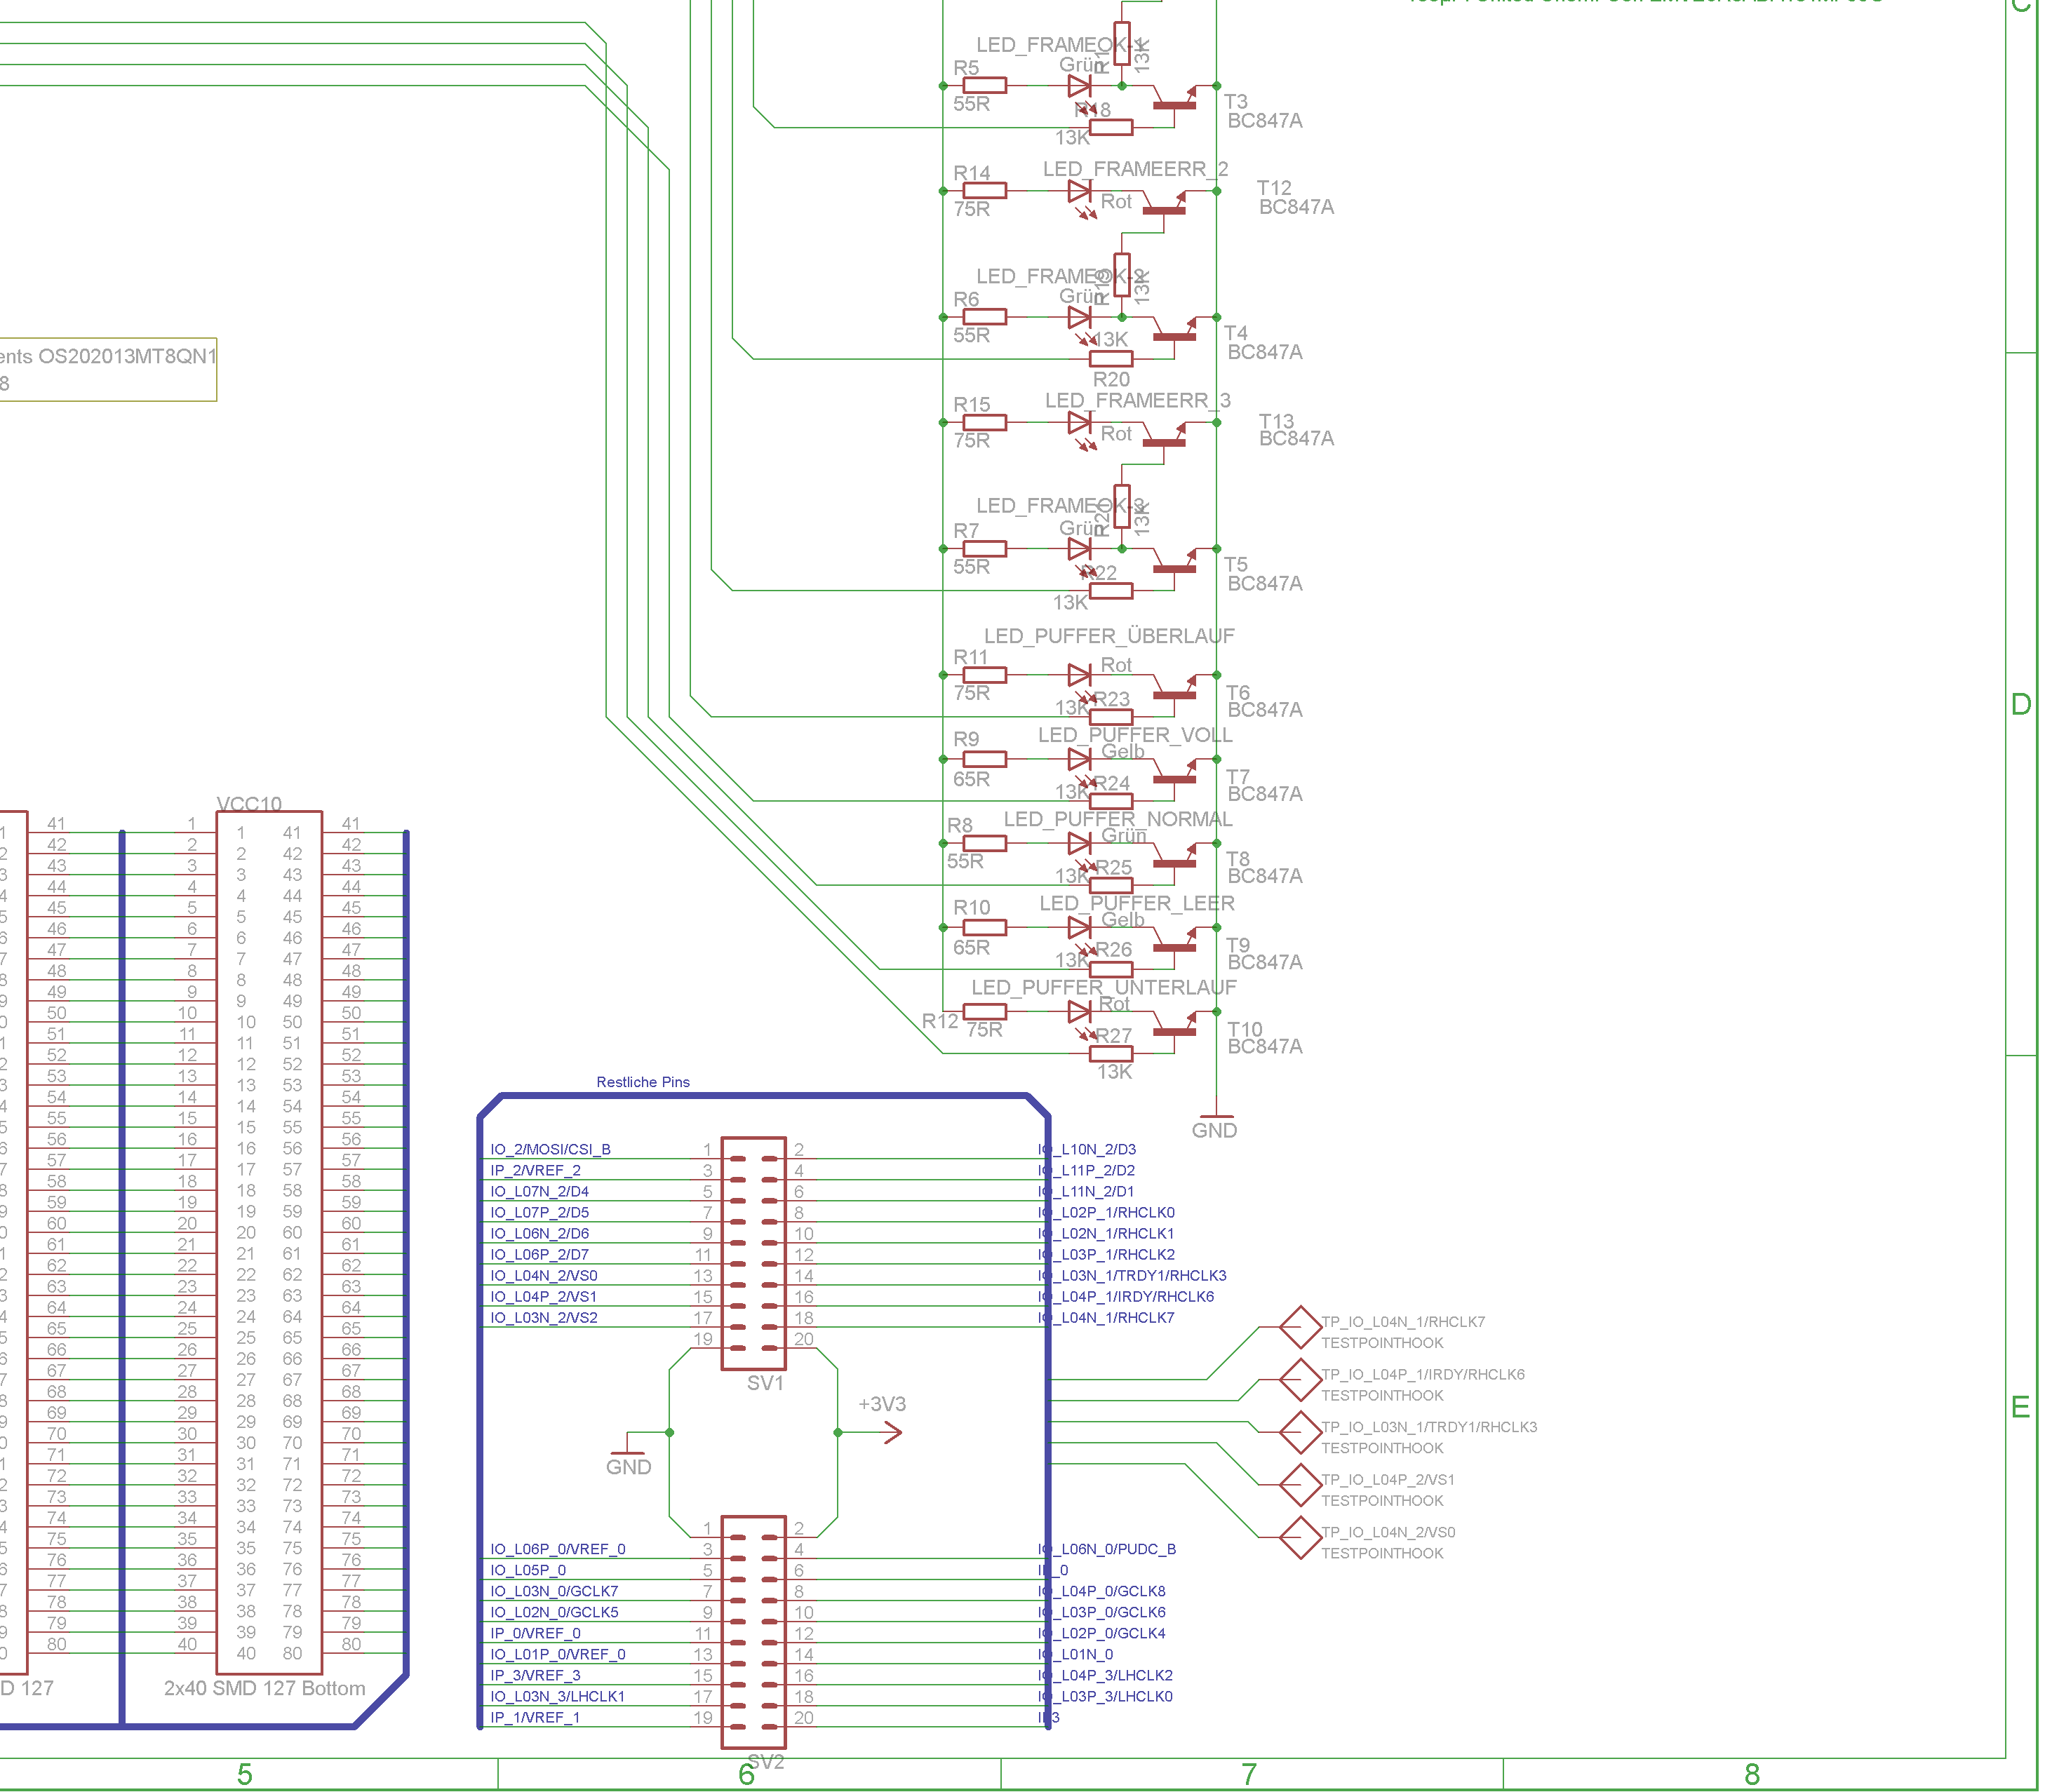
\includegraphics[width=\linewidth]{Medien/schaltplan4.png}
		\clearpage
		
		
	\section{Platinenlayout/Bestückungsplan}
		\subsection{Top Layer}
		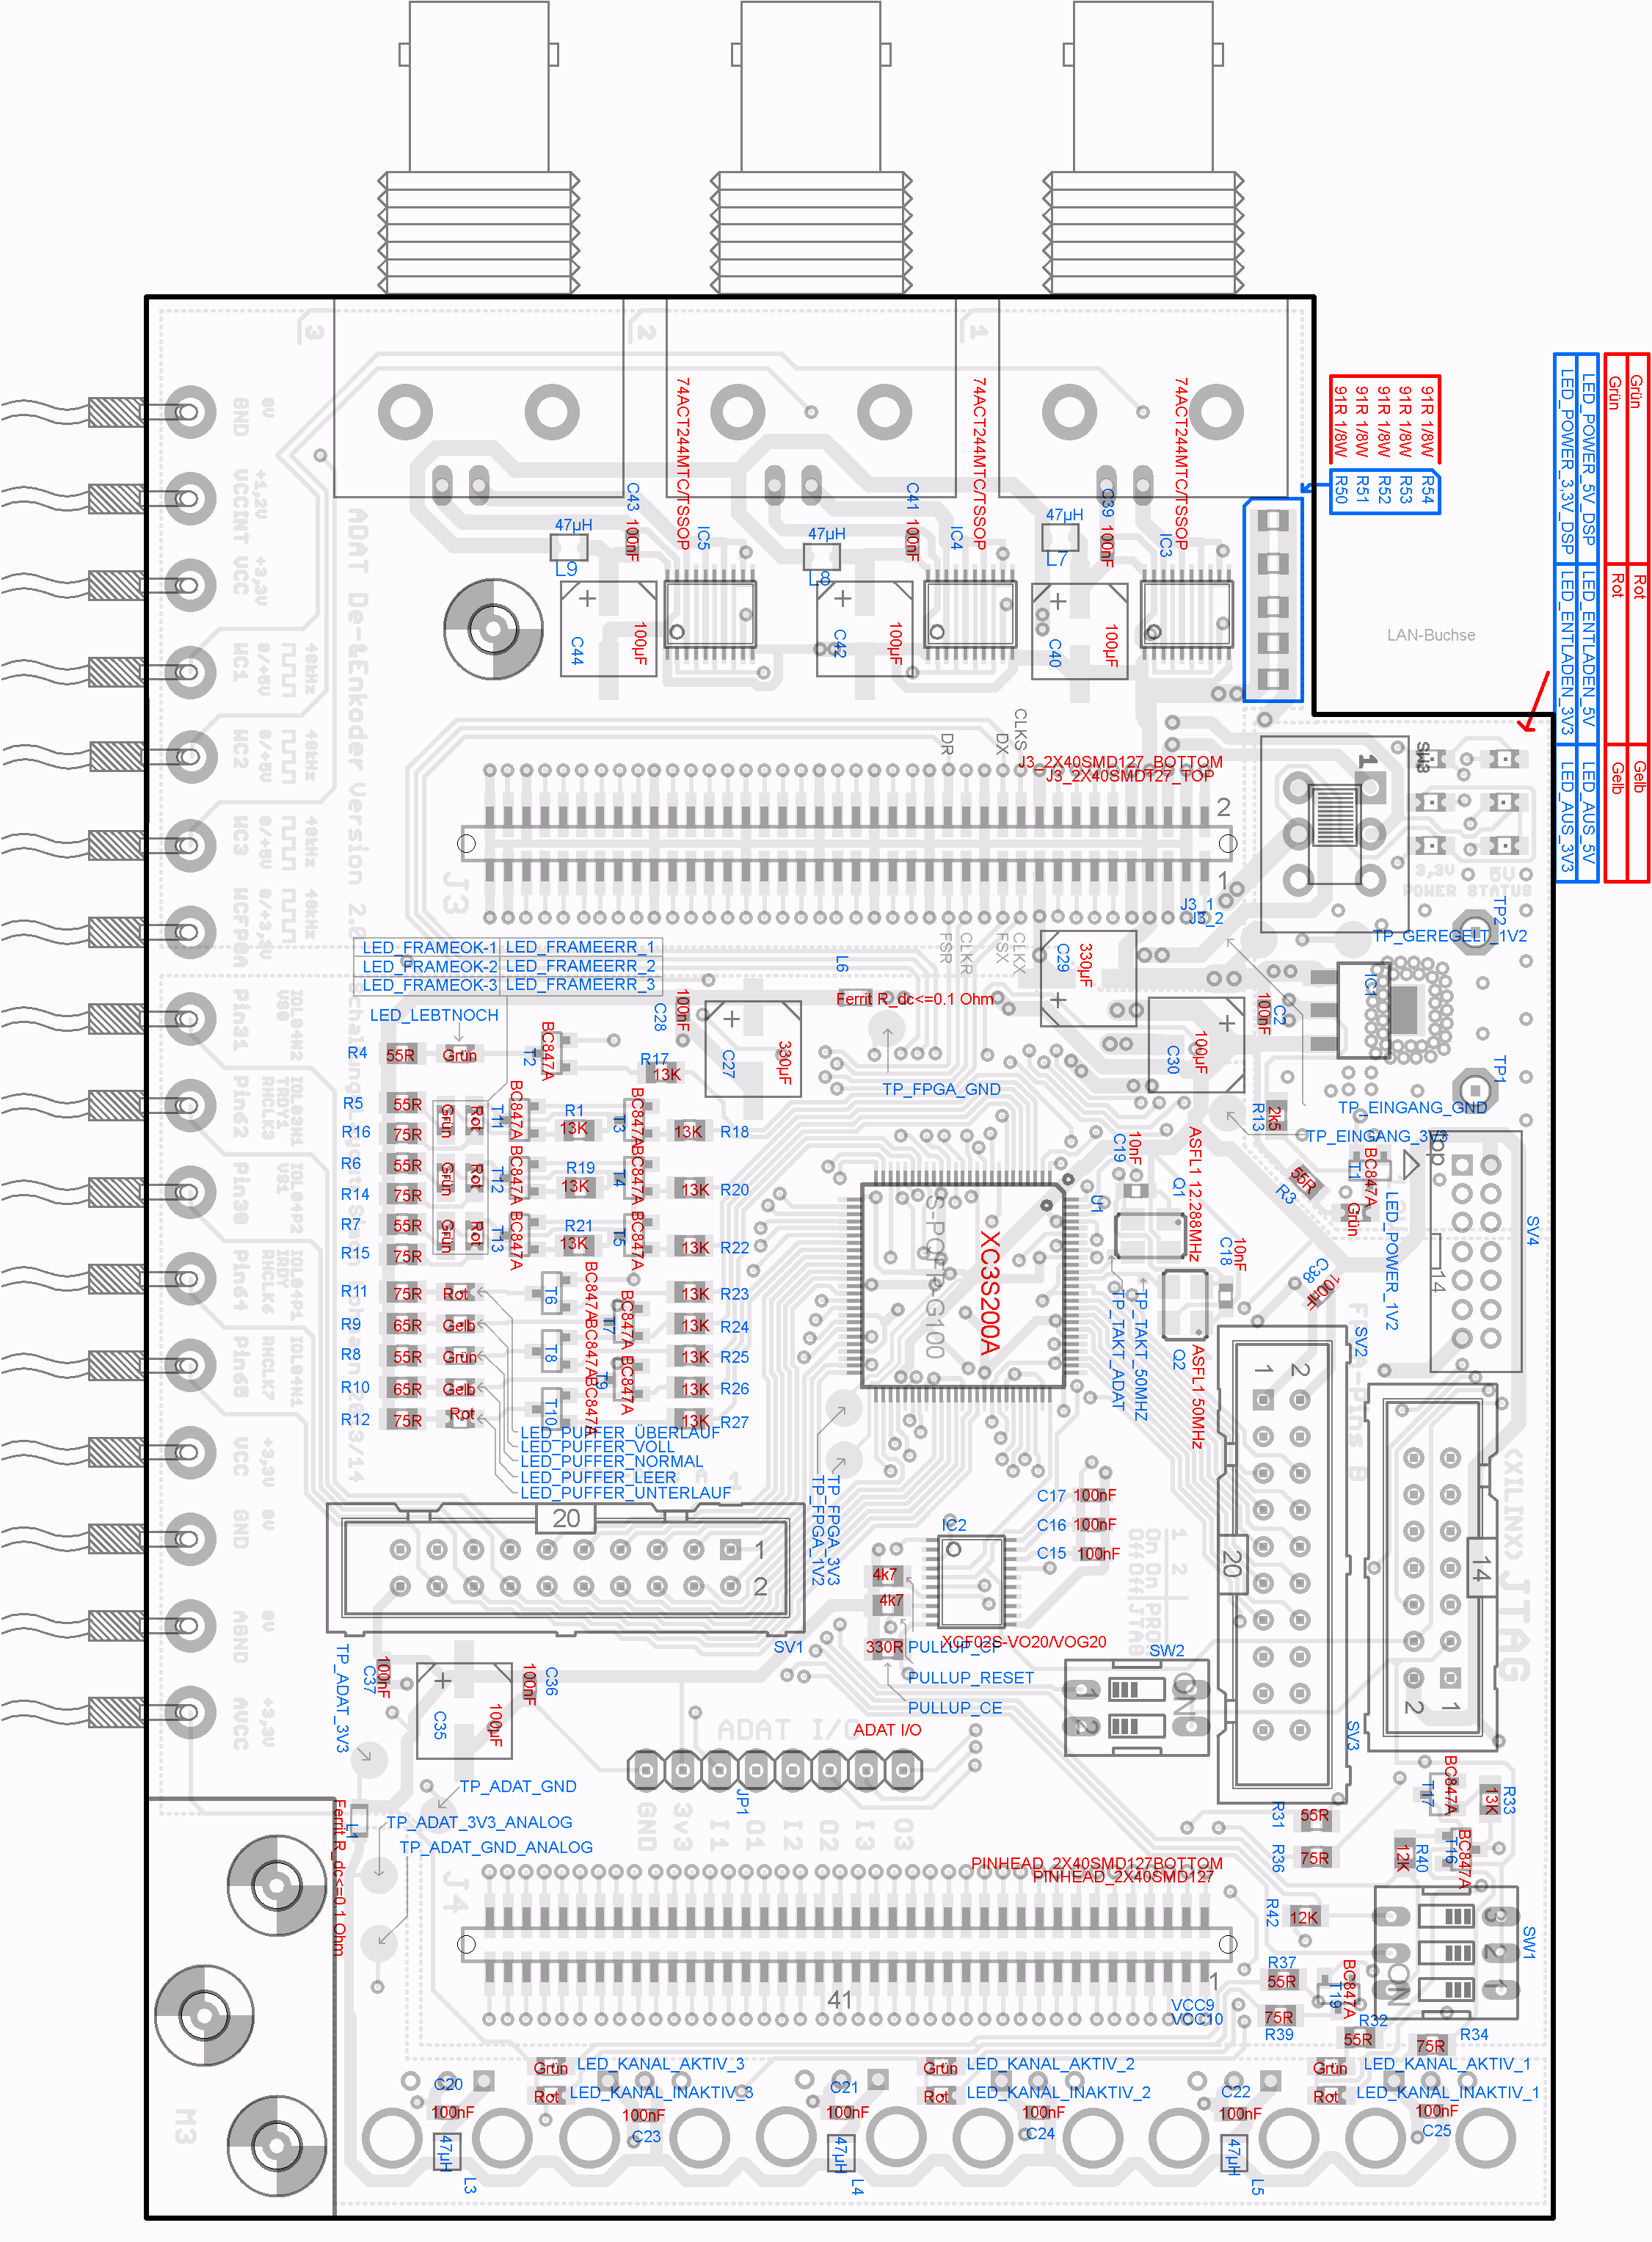
\includegraphics[width=0.85\linewidth]{Medien/bestueckungtop.png}
		\subsection{Bottom Layer}
		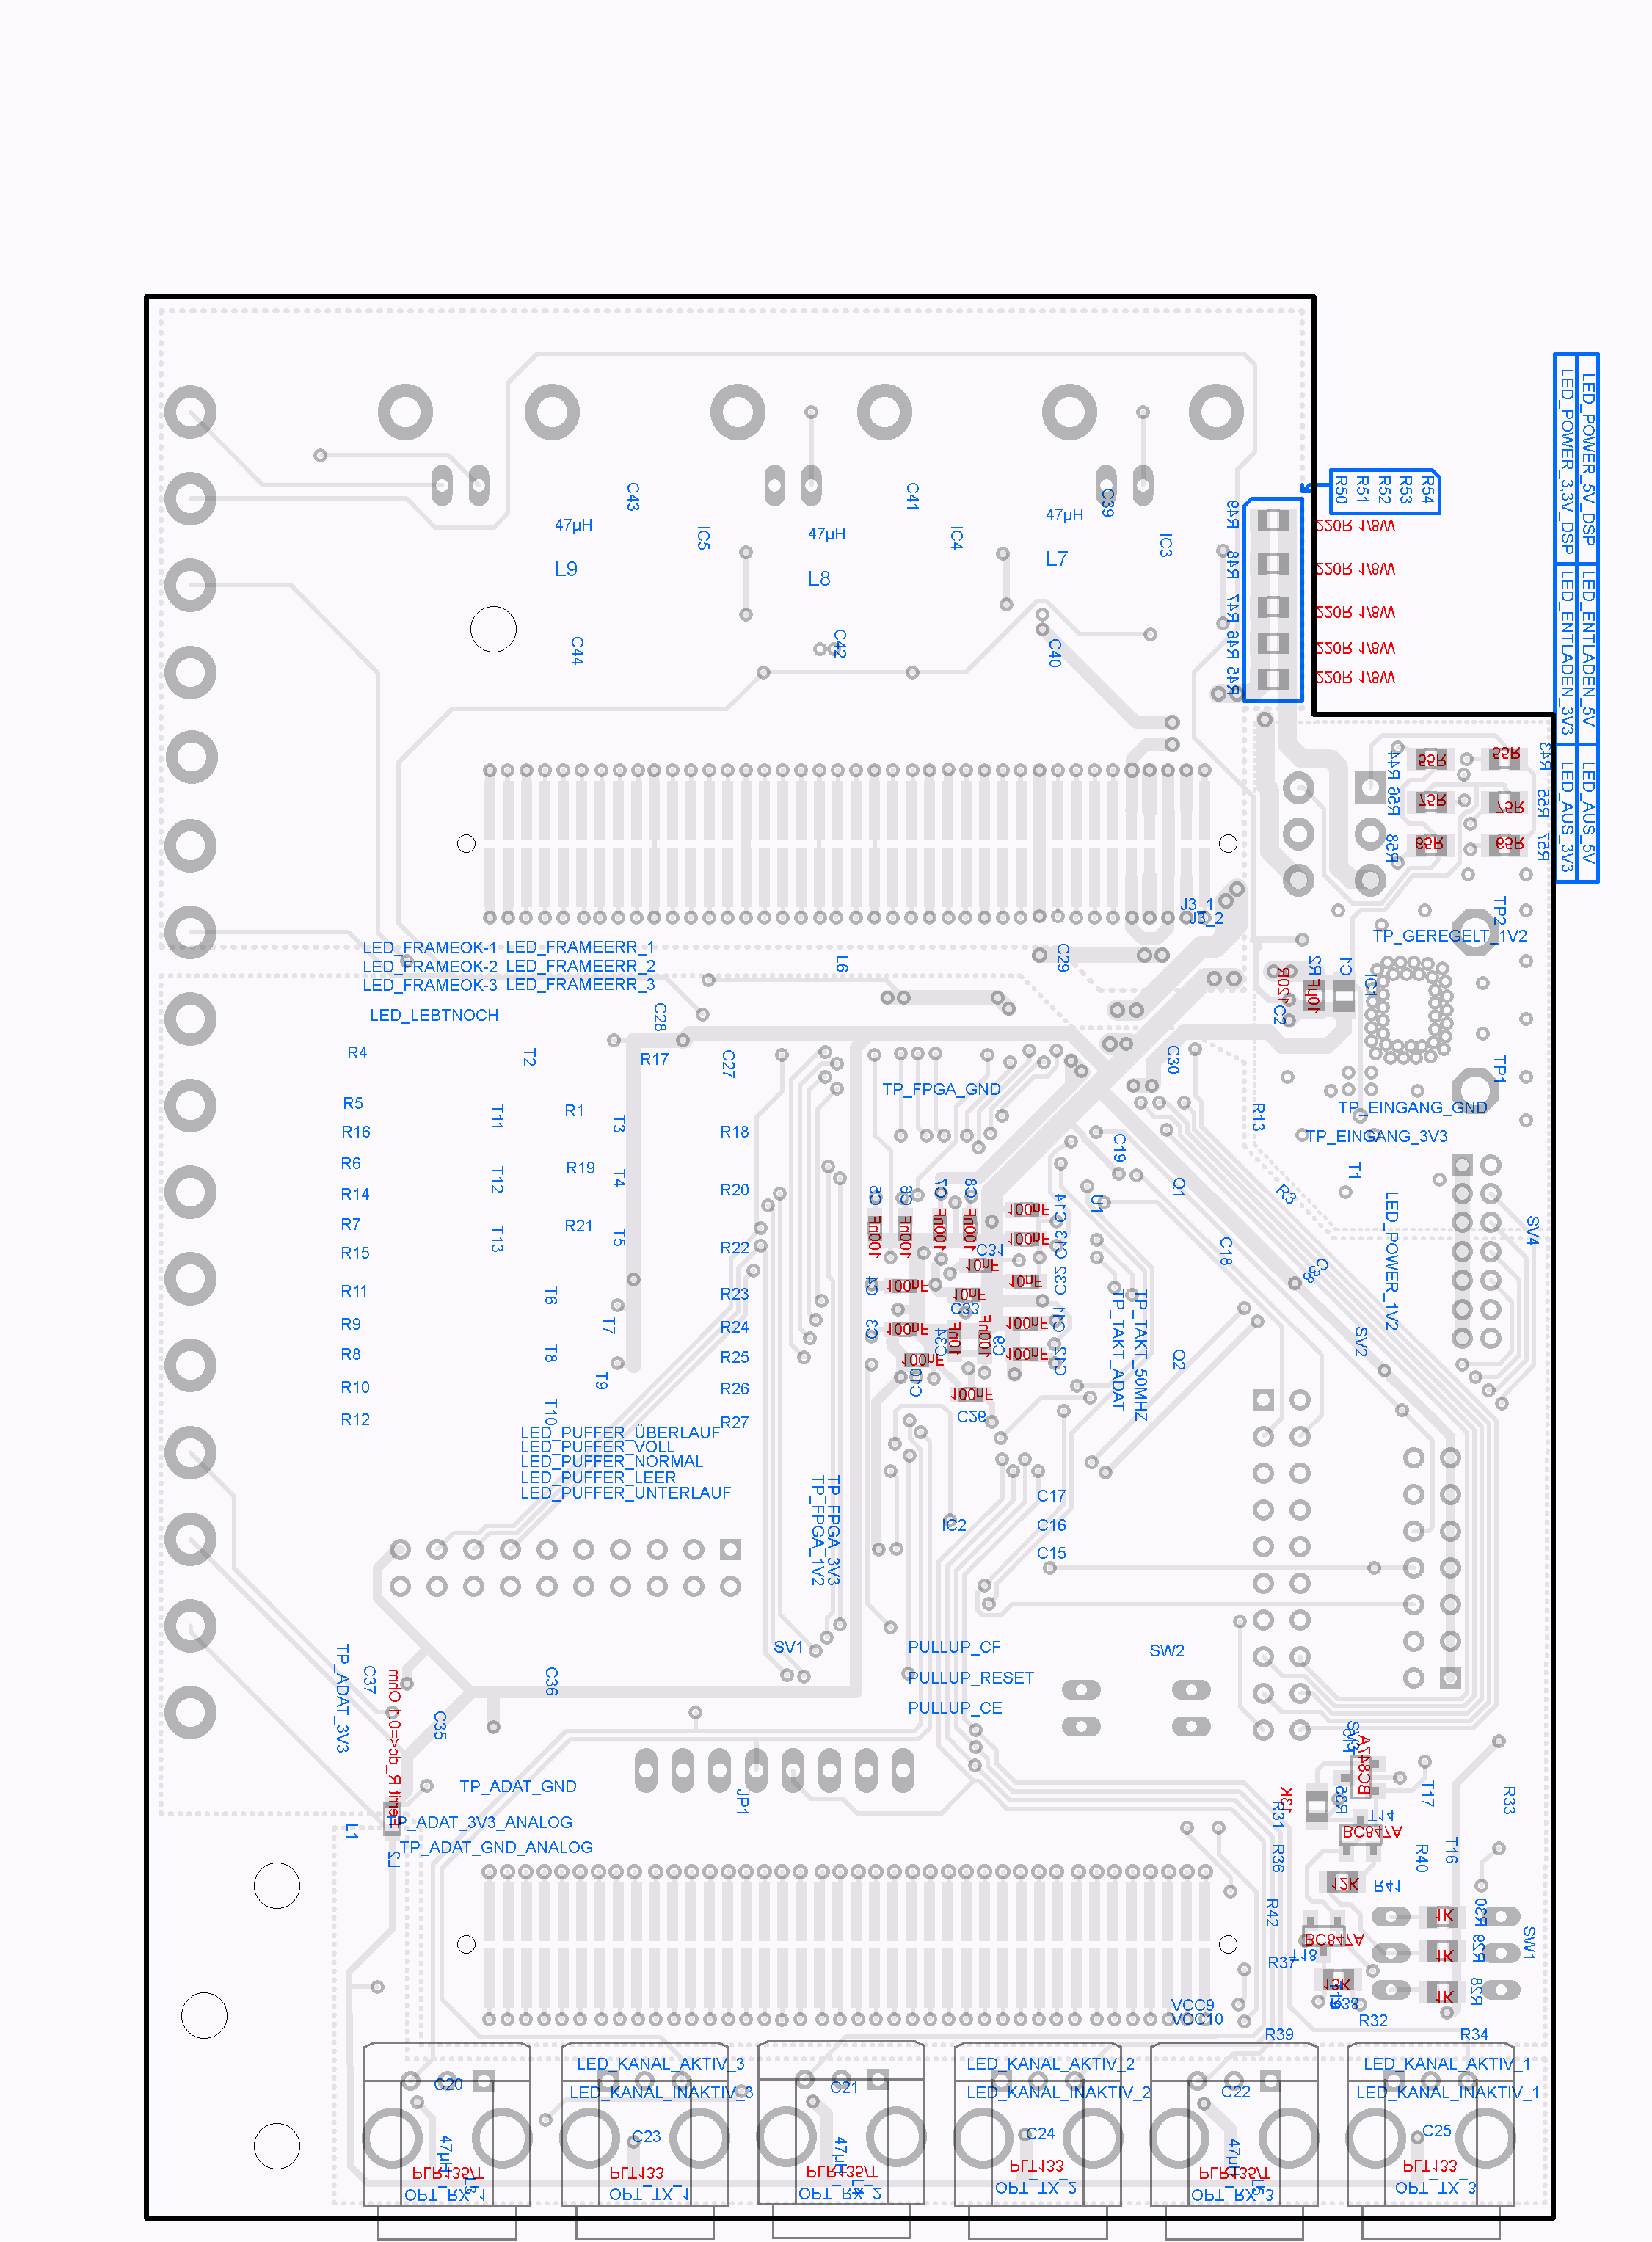
\includegraphics[width=0.85\linewidth]{Medien/bestueckungbottom.png}

%	\chapter{Messreihen}
	\blindtext
	%% Version 2023-08-21
%% LaTeX-Vorlage für Abschlussarbeiten
%% Erstellt von Nils Potthoff, ab 2020 erneuert und ausgebaut von Simon Lohmann
%% Lehrstuhl Automatisierungstechnik/Informatik Bergische Universität Wuppertal
%%%%%%%%%%%%%%%%%%%%%%%%%%%%%%%%%%%%%%%%%%%%%%%%%%%%%%%%%%%%%%%%%%%%%%%%%%%%%%%%

\chapter{Sourcecode}
	\begin{lstlisting}[language=C, caption={Ein Beispielhafter Quellcode}]
#include <stdio.h>

int main(void){
	printf("Hello World!\n");
	
	return 0;
}
	\end{lstlisting}


	%% Version 2023-08-21
%% LaTeX-Vorlage für Abschlussarbeiten
%% Erstellt von Nils Potthoff, ab 2020 erneuert und ausgebaut von Simon Lohmann
%% Lehrstuhl Automatisierungstechnik/Informatik Bergische Universität Wuppertal
%%%%%%%%%%%%%%%%%%%%%%%%%%%%%%%%%%%%%%%%%%%%%%%%%%%%%%%%%%%%%%%%%%%%%%%%%%%%%%%%

\chapter{Fragen und Antworten (FAQs)}
	\label{sec:anhang:faq}
	\emph{engl.: Häufig stellte Fragen}
	
	\emph{In \ref{FAQ:Vorlage} gibt es die FAQ speziell zu dieser Vorlage und dem Umgang damit.}
	
	\emph{In \ref{FAQ:LaTeX} werden typische Anfängerfragen zum Thema \LaTeX{} behandelt.} 
	
	\section{Zu dieser Vorlage}\label{FAQ:Vorlage}
		\subsection{Was brauche ich?}
			\subsubsection{Diese Vorlage}
			Die Vorlage wird als komprimiertes Archiv verteilt. Dieses muss zuerst entpackt werden.
			
			\subsubsection{Eine LaTeX-Distribution}
			Je nach Betriebssystem gibt es unterschiedliche Pakete, in denen \LaTeX zusammen mit den am häufigsten benutzten Paketen zu einer sogenannten \emph{\LaTeX-Distribution} zusammengefasst ist.
%			
			\TeX Live und MiKTeX sind die am häufigsten genutzten Varianten:
			
			\paragraph{TeX Live}~\\
			\fbox{Linux} \fbox{Windows} \fbox{MacOS\footnotemark}\footnotetext{für MacOS gibt es auch noch die speziell abgestimmte Variante \emph{MacTeX}, welche auf \emph{\TeX Live} aufbaut} \fbox{FreeBSD} \fbox{NetBSD} \fbox{Solaris}
			\hfill
			\url{http://tug.org/texlive/}
			\medskip
			
			\noindent Wird in den vielen Linux-Distributionen schon mitgeliefert und über den Linux-Paketmanager automatisch aktualisiert.
			%				
			Unter Ubuntu/Mint/Debian kann man es z.B. über das Terminal mit  
			\lstinline|sudo apt install texlive| installieren.
			%				
			Je nach Anwendung gibt es verschieden große Pakete. Mit \lstinline|texlive| installiert man ein einfaches TeX-System mit häufig genutzten Paketen. Dies ist für die meisten Anwendungsfälle ausreichend.
			%				
			\lstinline|texlive-base| wäre die Minimalinstallation, alle weiteren Pakete müssen von Hand installiert werden.
			%				
			\lstinline|texlive-full| enthält alle Pakete. Dafür braucht es natürlich auch am meisten Speicherplatz.
			
			\paragraph{MiKTeX}~\\
			\fbox{Linux} \fbox{Windows} \fbox{MacOS}
			\hfill
			\url{https://miktex.org/download}
			
			\noindent Lädt Pakete nur auf Anfrage, braucht also potenziell weniger Speicherplatz.
			Bei der Installation wird gefragt, was passieren soll, wenn MiKTeX bemerkt dass ein Paket fehlt:
			\begin{description}
				\item[Nicht installieren] Fehlende Pakete werden nicht automatisch installiert -- das muss man also selber machen. \textit{(Für Anfänger nicht empfohlen)}
				\item[Nachfragen] Sobald ein Paket fehlt, öffnet MiKTeX ein Fenster in dem man auswählen kann, ob das Paket installiert werden darf. Einfach und transparent. Am Anfang wird man aber möglicherweise ziemlich oft gefragt, bis alle Pakete heruntergeladen wurden.
				\item[Automatisch installieren] Fehlende Pakete werden ohne Nachfrage beim Nutzer automatisch installiert. Einfach, aber intransparent.
			\end{description}
			
			Man kann diese Option in den Einstellungen von MiKTeX auch später noch ändern.
			
			\subsubsection{Einen (LaTeX-) Editor}
			\emph{Weil \LaTeX-Quellcode auch nur ganz normaler Text ist, kann im Prinzip jeder beliebige Text-Editor\footnote{Nur bitte nicht Word, Writer etc. Das sind keine Text-Editoren!} benutzt werden.}
			\medskip
			
			Viel einfacher (und übersichtlicher) wird es aber, wenn man einen \LaTeX-Editor benutzt.
			Diese Programme kennen in der Regel die meisten Befehle und können diese automatisch vervollständigen, bieten Vorschaufunktionen, einfaches Kompilieren und vieles mehr.
			
			
			Empfehlenswert ist z.B. \emph{TeXstudio\footnote{\url{https://www.texstudio.org/}, verfügbar für Linux, Windows \& Mac OS}}, in dem ich diesen Text hier gerade schreibe und schon diverse Vorlagen und Pakete entwickelt habe. Es enthält eine Autovervollständigung der gängigen \LaTeX-Befehle, eine einfache Rechtschreibprüfung und viele Hilfsfunktionen zum Finden von Symbolen, Formatieren von Tabellen und so weiter...
			\medskip
			
			\emph{Besonders praktisch finde ich die Option, direkt per Strg+Klick im PDF an die entsprechende Stelle im Quellcode zu springen (das geht natürlich auch anders herum). Oder mit Strg+Klick auf einen Paketnamen die entsprechende Dokumentation zu öffnen. Oder sich z.B. die Vorschau einer Formel direkt im Quellcode anzeigen zu lassen. Und es gibt noch so viel mehr...}
			
			\subsubsection{Eine Literaturverwaltung (optional)}
			Die Literaturliste kann man in einem \LaTeX-Editor schon hinreichend gut bearbeiten.
			%			
			Literaturverwaltungsprogramme können einem die Arbeit aber erleichtern.
			%			
			Frei verfügbar ist z.B. das Programm \emph{JabRef}\footnote{Läuft unter Linux, Windows und Mac OS, \url{http://www.jabref.org/}}.
			Dieses kann auch diverse Wissenschaftliche Online-Verzeichnisse durchsuchen, eignet sich (bedingt) also auch zur Literaturrecherche.
		
			
		\subsection{Titelblatt und Einstellungen ändern}\label{FAQ:Einstellungen}
			Die für Benutzer gedachten Einstellungsmöglichkeiten finden sich in der Datei \lstinline|Einstellungen.tex|.
%			
			Damit kann man \zb{} die Angaben auf der Titelseite ändern, zwischen einseitigem und doppelseitigem Layout wählen oder entscheiden, welche Verzeichnisse generiert werden sollen und vieles mehr. Alle Optionen sind dort ausführlich kommentiert.
			
		\subsection{Literatur/Quellen}
			Die Literatureinträge werden von dieser Vorlage aus der Datei \lstinline|Literatur.bib| geladen.
			Hat sich etwas an dieser Datei geändert, muss das Literaturverzeichnis neu kompiliert werden. (siehe \ref{FAQ:kompilieren:literatur} \emph{\nameref{FAQ:kompilieren:literatur}})
			
		\subsection{Glossareinträge, Abkürzungen, Akronyme}
			werden in der Datei \lstinline|Glossar.tex| eingetragen.
		
		\subsection{Im PDF sind am Anfang mehrere leere Seiten}
			Je nachdem ob Ihr in \lstinline|Einstellungen.tex| das einseitige oder das doppelseitige Layout gewählt habt, werden leere Seiten zwischen Kapiteln generiert.
			Das sieht im PDF erst mal seltsam aus, ist aber Absicht:
			%		
			So fängt \zb{} der Inhaltsteil auf der rechten Seite an (das ist eine übliche Konvention).
			Damit dann auf der linken Seite nicht noch der Rest vom Inhaltsverzeichnis steht, was schon mal etwas seltsam aussehen kann, wird dafür gesorgt, dass die erste linke Seite vor dem Start des Texts leer ist. Endet das Inhaltsverzeichnis auf der linken Seite, ergibt sich zusätzlich noch eine leere rechte Seite.
			
			Bei Aufgabenstellung, ggf. Verlängerung und Eidesstattlicher Erklärung handelt es sich jeweils um allein stehende Elemente, daher wird auch hier jeweils dafür gesorgt, dass die linke Seite daneben leer bleibt.
		
		\subsection{Seitenränder springen hin und her}
			Im doppelseitigen Layout gibt es einen inneren und einen äußeren Rand.
			\medskip
			
			\textit{In den \hyperref[FAQ:Einstellungen]{Einstellungen} kann bei Bedarf auch ein einseitiges Layout gewählt werden.}
		
		\subsection{Seitenzahlen springen hin und her}
			Im doppelseitigen Layout gibt es einen inneren und einen äußeren Rand.
			Die Seitenzahlen stehen immer am äußeren Rand der Seite.
			\medskip
			
			\textit{In den \hyperref[FAQ:Einstellungen]{Einstellungen} kann bei Bedarf auch ein einseitiges Layout gewählt werden.}
			
		\subsection{Die Druckerei zählt S/W-Seiten als Farbseiten}
			\textit{Farbseiten sind meist deutlich teurer als Schwarz-Weiß bzw. Graustufen-Seiten.
			Es kann also sinnvoll sein, wenn nur die Seiten mit farbigen Bildern etc. als Farbseiten gedruckt werden. Viele Thesis-Druckereien und Copyshops haben dafür eine Software, die Farbseiten automatisch erkennen kann\footnote{Oder das zumindest können sollte ;-)}.}
			
			Meistens funktioniert das mit dieser Thesisvorlage einwandfrei.
			Einige wenige Druckereien verhalten sich diesbezüglich aber \emph{etwas seltsam}.
			Falls eure Druckerei Probleme macht, könnt ihr in der Datei \emph{Einstellungen.tex} den Parameter \lstinline|\colormodel| anpassen.
			
			Faustregel für \lstinline|\colormodel|:
			\begin{itemize}
			\item erst bei der Standardeinstellung \lstinline|cmyk| lassen. Das ist das professionelle Druckformat.
			\item wenn die Druckerei Probleme macht, auf \lstinline|rgb| umstellen. Hat in einem uns bekannten Fall schon mal geholfen.
			\item wenn die Druckerei immer noch Probleme macht, auf \lstinline|gray| umstellen.
			\end{itemize}

	\clearpage
	\section{Zu \LaTeX{} allgemein}\label{FAQ:LaTeX}
		\subsection{Aus \LaTeX{} wird ein PDF}
			\LaTeX-Quellcode wird kompiliert, dass heißt ein spezielles Programm (der \emph{Compiler}) liest den Quellcode und erstellt daraus ein Dokument im Zielformat.
			Je nach Compiler und dessen Einstellungen können dabei unterschiedliche Zielformate herauskommen.
%			
			Einer der wichtigsten Compiler ist \emph{Pdf\LaTeX}. Er erstellt aus dem Code ein PDF-Dokument. Dieses kann dann einfach betrachtet, gedruckt, kommentiert oder auf einem Datenträger der Thesis beigelegt werden.
			
			\emph{Praktisch alle Druckereien nehmen PDF-Dokumente an.
			Mit einem Writer- oder Word-Dokument, LaTeX-Code oder anderen Datei-Formaten wollen die Druckereien dagegen häufig lieber nichts zu tun haben\footnote{Im schlimmsten Fall wird der Druckauftrag abgelehnt. Alternativ muss evtl. einen Aufpreis für die Konvertierung gezahlt werden. Mit einem PDF ist man dagegen bei praktisch allen seriösen Anbietern auf der sicheren Seite.}}
			
		\subsection{\LaTeX{} kompilieren}
			Die Thesis kann im Terminal mit dem Befehl \lstinline|pdflatex Thesis.tex| kompiliert werden.
			In \emph{TeXstudio} geht das mit einem Klick auf den Kompilieren-Button oder mit der Taste \fbox{F5}.
			
			In manchen Fällen muss man zwei mal kompilieren, mehr dazu in Abschnitt \ref{FAQ:kompilieren:zweimal} \emph{\nameref{FAQ:kompilieren:zweimal}}.
		\subsection{Literaturverzeichnis kompilieren}\label{FAQ:kompilieren:literatur}	
			Das Literaturverzeichnis wird in der Regel von einem separaten Programm verarbeitet (z.B. BibTeX, BibLaTeX oder Biber).
			%In dieser Thesisvorlage wird BibLaTeX verwendet, das Backend ist BibTeX (so passen die Standardeinstellungen von TeXstudio direkt).
			\medskip
			
			Dieses muss explizit aufgerufen werden.
			In \emph{TeXstudio} geht dass z.B. mit der Taste \fbox{F8}, im Terminal per \lstinline|bibtex Thesis.aux|.
			
			Danach muss dann das \LaTeX-Dokument (in \emph{TeXstudio} mit \fbox{F5}) kompiliert werden.
			\bigskip
			
			\hrule
			\medskip
			\noindent \textbf{Im Worstcase\footnote{alles hat sich geändert} muss man}:
			\begin{enumerate}
			\item \LaTeX-Code kompilieren \emph{(damit bekannt ist, welche Quellenverweise es gibt)}
			\item Literatur kompilieren \emph{(Quellen zusammenstellen)}
			\item \LaTeX-Code kompilieren \emph{(Layout des Dokuments, Verzeichnisse vorbereiten)}
			\item \LaTeX-Code kompilieren \emph{(Verzeichnisse korrekt setzen)}
			\end{enumerate}
			In der Praxis ist das aber kein großes Problem, da man beim Arbeiten an dem Dokument meist nach Bedarf kompiliert...
			\hrule
		
		\subsection{Zwei mal kompilieren (und warum)}\label{FAQ:kompilieren:zweimal}
			\textit{
				\begin{itemize}\itemsep=0pt
					\item Das neue Kapitel ist nicht im Inhaltsverzeichnis aufgeführt?
					\item Der Verweis auf ein Bild zeigt auf die falsche Seite?
				\end{itemize}
			}
			
			\begin{center}
				Lösung: Zwei mal kompilieren.
				\bigskip
				
				Aber warum eigentlich?
			\end{center}
			
			
			Normalerweise wird der \LaTeX-Code einmal von vorne nach hinten durchgegangen und dabei kompiliert.
%			
			Am Beispiel des Inhaltsverzeichnis wird direkt klar, dass damit bestimmte Dinge nicht möglich sind:
				Wenn das Inhaltsverzeichnis vorne im Dokument gesetzt werden soll, weiß \LaTeX{} zu diesem Zeitpunkt noch gar nicht, auf welcher Seite die Kapitel stehen werden und welche Kapitel es überhaupt gibt -- schließlich folgen diese erst später im Quellcode.
			
			Stattdessen läuft der \LaTeX-Compiler einmal durch das gesamte Dokument und merkt sich dabei, welche Kapitel existieren und auf welchen Seiten diese begonnen haben.
				Diese Information wird dann in eine Datei gespeichert\footnote{Deshalb liegen neben dem eigentlichen \LaTeX-Dokument und der Literaturdatei nach dem Kompilieren noch so viele andere Dateien mit Endungen wie z.B. \lstinline|.aux| oder \lstinline|.toc| herum}.
%			
			Im zweiten Durchlauf werden diese Informationen wieder eingelesen und verwendet um das Inhaltsverzeichnis zu erstellen, d.h. das Inhaltsverzeichnis hinkt quasi einen Kompilierschritt hinterher.
			\bigskip
			
			\noindent Das gleiche gilt auch für
			\begin{itemize}
			\item Verweise/Referenzen (bzw. alles was mit Seitenzahlen zu tun hat)
			\item alle anderen Verzeichnisse, z.B. Abbildungsverzeichnis, Tabellenverzeichnis, Literaturverzeichnis.
			\end{itemize}
		
		

		
		\subsection{Floating-Umgebungen}\label{sec:wissen:float}
			\textit{Hilfe, mein Bild/meine Tabelle/... ist nicht wo es sein soll!} --
	%		
			Bilder, Tabellen usw. sind in \LaTeX{} sogenannte \emph{Floating-Umgebungen}, d.h. sie sind nicht fest an einem Platz, sonderen werden beim Kompilieren so verschoben, dass die Seite gut aussieht.
	%		
			Nun ist \emph{was gut aussieht} nicht unbedingt für jeden gleich, und es gibt auch Fälle in denen \LaTeX{} sich scheinbar sehr seltsam entscheidet.
			Daher kann man in eckigen Klammern ggf. Präferenzen für die Positionierung angeben, die \LaTeX{} dann als Orientierung nimmt - im Zweifelsfall aber auch ignorieren darf:
			
			\begin{description}
			\item[t] bitte oben auf die Seite
			\item[b] bitte unten auf die Seite
			\item[h] bitte hier an dieser Stelle im Text
			\item[p] bitte auf eine eigene Seite packen, auf der nur andere Floats sein dürfen
			\item[!] \LaTeX soll seine eigenen Regeln zum guten Platzieren von Floats ignorieren
			\end{description}
			
			\textbf{Tipp:}
			Mit \lstinline|\clearpage| wird nicht nur die aktuelle Seite beendet und für weitere Inhalte eine neue angefangen. Es werden auch alle noch offenen Float Objekte ausgegeben. Der Befehl bietet also eine einfach Möglichkeit dafür zu sorgen, das Objekte nicht in den nächsten Abschnitt mitgenommen werden.
		
	
		\subsection{Leerzeichen nach einem Befehl fehlt}
			\subsubsection*{Das Problem}
				Schreibt man einen Satz wie z.B. \emph{Ich benutze \LaTeX, weil \LaTeX für Formelsatz super ist.} so fällt auf, dass zwischen \emph{\LaTeX{}} und \emph{für} das Leerzeichen fehlt.			
				Habe ich es einfach nur vergessen?
				
				Nein, hier ist der Quellcode:
				\bigskip
				
				\lstinline[language=thesis-latexbeispiel, showspaces=true]|Ich benutze \LaTeX, weil \LaTeX für Formelsatz super ist.|
				\bigskip
			
				Wie man sieht, steht hinter dem zweiten \lstinline[language=thesis-latexbeispiel]|\LaTeX| eindeutig ein Leerzeichen. Dieses fällt aber weg, weil Befehle in \LaTeX normalerweise grundsätzlich Parameter erwarten, also das nächste Zeichen betrachten und schauen ob noch ein Parameter kommt. Bei fettgedrucktem Text wie \lstinline[language=thesis-latexbeispiel]|dieser \textbf{Text} ist fettgedruckt| (dieser \textbf{Text} ist fettgedruckt) ist das offensichtlich, bei \lstinline[language=thesis-latexbeispiel]|\LaTeX| halt nicht. Wie man bei genauem Hinschauen sieht, ist es beim ersten \lstinline[language=thesis-latexbeispiel]|\LaTeX| auch kein Problem, weil direkt ein Komma folgt. Lediglich Leerzeichen werden von solchen Befehlen \glqq gefressen\grqq, weil ein Leerzeichen erlaubt wäre.
				
				Dieses Verhalten ist auch durchaus sinnvoll, weil man manchmal nach einem \LaTeX-Befehl vielleicht auch gar kein Leerzeichen haben will. So ist z.B. \lstinline|\LaTeXbefehl| kein gültiger \LaTeX befehl, und eigentlich wollten wir hier ja auch nur \lstinline[language=thesis-latexbeispiel]|\LaTeX| und \lstinline|befehl| aneinanderhängen. Folglich kommt zwischen \lstinline[language=thesis-latexbeispiel]|\LaTeX| und \lstinline|befehl| ein Leerzeichen, an dem \LaTeX erkennt, wo der Befehl zu Ende ist und der Text weitergeht. Weil das Leerzeichen aber nur markiert, wo der \LaTeX Befehl endet, taucht es im Text nicht auf.
			\subsubsection*{Die Lösung}
				In solchen Fällen (oder immer, es schadet jedenfalls nie) einfach \lstinline[language=thesis-latexbeispiel]|\LaTeX{}| schreiben, also leere Parameterklammern hinzufügen. So ist direkt klar, wo der Befehl aufhört und das Leerzeichen wird nicht mehr \glqq gefressen\grqq:
				\bigskip
				
				\emph{Ich benutze \LaTeX, weil \LaTeX{} für Formelsatz super ist.}
				\medskip
				
				\lstinline[language=thesis-latexbeispiel, showspaces=true]|Ich benutze \LaTeX, weil \LaTeX{} für Formelsatz super ist.|
              % Fragen und Antworten zur Vorlage und zu LaTeX
	\chapter{\LaTeX-Beispiele}
\label{sec:anhang:latex-beispiele}
	\emph{Dieses Kapitel beinhaltet Beispiele und kurze Erklärungen zu verschiedenen \LaTeX-Funktionen die in einer wissenschaftlichen Ausarbeitung nützlich sein könnten.%
%	Wie diese konkret benutzt werden, kann man im \LaTeX-Quellcode der Thesisvorlage %(Datei \lstinline|LaTeX-Beispiele.tex|)
%	 sehen.
	 }
		
	\section{Kapitel, Abschnitte, Paragraphen}\label{sec:chapter-section-paragraph}
		Kapitel werden mit \lstinline|\chapter{Kapitelname}| erstellt.
		Als nächste Ebenen folgen \lstinline|\section{title}|, \lstinline|\subsection{title}| und \lstinline|\subsubsection{title}|.
		Reicht das immer noch nicht, gibt es auch noch \lstinline|\paragraph{title}| und für den aller äußersten Notfall\footnote{Wer so viele Hierarchieebenen benötigt macht in der Regel etwas falsch -- Selbst außergewöhnlich lange Bachelor- und Master-Thesen sind normalerweise nicht so umfangreich, dass Subparagraphen nötig werden} sogar noch \lstinline|\subparagraph{title}|.
		\begin{vorlagenbeispiel}
			\subsection{Subsection}
				Hier sind wir in einer Subsection.
				\subsubsection{Subsubsection}
					Hier sind wir in einer Subsubsection.
					\paragraph{Paragraph}
						Hier sind wir in einem Paragraph.
%						\subparagraph{Subparagraph}
%							Hier sind wir in einem Subparagraph.
		\end{vorlagenbeispiel}
		
	\section{Textauszeichnung}
		\begin{vorlagenbeispiel}
			Text kann man zum Beispiel \textbf{Fett}, \textit{Kursiv} oder \underline{Unterstrichen} hervorheben. Das geht aber auch mit \textsc{Kapitälchen}, \texttt{Dicktengleicher Schrift} oder \textsf{Serifenloser Schrift}.
		\end{vorlagenbeispiel}
		\begin{lstlisting}[keywords={textbf, textit, underline, textsc, texttt, textsf}]
Text kann man zum Beispiel \textbf{Fett}, \textit{Kursiv} oder \underline{Unterstrichen} hervorheben. Das geht aber auch mit \textsc{Kapitälchen}, \texttt{Dicktengleicher Schrift} oder \textsf{Serifenloser Schrift}.
		\end{lstlisting}
					
	\section{Fußnoten}
		\begin{vorlagenbeispiel}
		Ein Text kann Fußnoten\footnote{Wie z.B. diese hier} enthalten.
		\end{vorlagenbeispiel}
		Diese werden mit \lstinline|\footnote{text}| gesetzt. Formatierungen in der Fußnote sind grundsätzlich kein Problem%
		\footnote{%
			\color{red}Dies ist eine besonders \textbf{fette Fußnote} in rot.
		}.
%		
		Aber Vorsicht: Manche Befehle wie \zb \lstinline|\lstinline| können nicht ohne weiteres/nicht immer in einer Fußnote gesetzt werden\footnote{Der Grund dafür lässt sich unter \url{https://www.texfaq.org/FAQ-verbwithin} nachlesen}.
	
	\section{Zitate \& Literaturangaben}
		\subsection{Zitieren}
			Korrektes Zitieren ist in der Wissenschaft \emph{(und auch sonst)} äußerst wichtig und daher Pflicht.
%			\medskip
%			
			Bei allem%
				\footnote{Basiswissen aus dem eigenen Fachbereich muss in der Regel nicht zitiert werden:
					Studierende der Elektotechnik müssen $U = R \cdot I$ nicht zitieren.
					Kunst-Studierende, die eine LED verwenden möchten und einen Vorwiderstand berechnen, bisher aber noch nie etwas von dieser Formel gehört haben, sollten dies hingegen schon.}%
			, was man von anderen übernommen hat, muss angegeben werden, woher es stammt und wer es verfasst/veröffentlicht hat.
				\medskip
					
			Auf diese Weise wird eindeutig gezeigt, dass eine Information aus einer anderen Quelle übernommen wurde.
			Übernimmt man Informationen, lässt aber den Quellenverweis weg, suggeriert man damit fälschlicherweise man sei selbst die Quelle.
			
			\textbf{%
				Dies macht die entsprechende Stelle dann zu einem Plagiat} -- in der Regel ein vernichtendes Urteil für jede Arbeit und normalerweise ein schneller Weg bei Thesis, Praktikum, Seminar \& co. in Schimpf und Schande durchzufallen!
%			}
			\medskip
		
			\emph{\paragraph{Keine Panik...}
				Wer grundsätzlich gewissenhaft zitiert, an einer Stelle aber mal eine Zitierklammer vergisst, fällt damit natürlich nicht direkt durch...}
				
			\emph{\paragraph{...aber bitte eigene Leistung zeigen}
				Wer alles korrekt zitiert, aber auch keinen eigenen Text schreibt\footnote{Soll alles schon mal vorgekommen sein...}, hat zwar kein Plagiat abgegeben (gut), aber auch keine eigene Leistung gezeigt (schlecht).
				\\
				Und eigene Leistung ist nun einmal das was bewertet wird ;)}
			\clearpage
				
		\subsection{Literaturverzeichnis}
			Literatur wird in der Datei \lstinline|Literatur.bib| angegeben und in der Thesis dann mit dem Befehl \lstinline[language=thesis-latexbeispiel]|\cite{literaturname}| zitiert\cite{thesis:vorlage} -- mehr dazu in \ref{sec:zitate-in-latex}:  \nameref{sec:zitate-in-latex}¸.
			\medskip
			
			Am einfachsten ist die Bearbeitung der Datei \lstinline|Literatur.bib| mit einem Literaturverwaltungsprogramm wie beispielsweise dem frei verfügbaren \href{https://www.jabref.org/}{\emph{JabRef}}
		
		\subsection{Zitate in \LaTeX}\label{sec:zitate-in-latex}
			Zitieren kann man auf viele Arten.
			Dabei reicht es aber nicht, den Text einfach nur in Anführungszeichen zu setzen, z.\,B. \enquote{Text}!
			Für ein korrektes Zitat muss immer auch die Quellenangabe erkennbar sein.
			Die Zitierklammer kann in einem Satz hinter eine übernommene Behauptung gesetzt werden:
			
			\begin{vorlagenbeispiel}
				\noindent Der AXI-Bus hat eine Datenbreite, die stets ein Vielfaches von acht Bit\cite{ARM:AMBA4AXI4StreamProtocol:v1_0} beträgt.
			\end{vorlagenbeispiel}
			\begin{lstlisting}[language=thesis-latexbeispiel, numbers=none]
Der AXI-Bus hat eine Datenbreite, die stets ein Vielfaches von acht Bit\cite{ARM:AMBA4AXI4StreamProtocol:v1_0} beträgt.
			\end{lstlisting}
			
			So richtig hilfreich wird ein Zitat natürlich erst, wenn wir dem Leser auch einen Hinweis geben, an welcher Stelle (also \zb{} in welchem Kapitel oder auf welcher Seite) er in der angegebenen Quelle suchen muss:
			
			\begin{vorlagenbeispiel}
				\noindent Der AXI-Bus hat eine Datenbreite, die stets ein Vielfaches von acht Bit\cite[S.42]{ARM:AMBA4AXI4StreamProtocol:v1_0} beträgt.
			\end{vorlagenbeispiel}
			\begin{lstlisting}[language=thesis-latexbeispiel, numbers=none]
Der AXI-Bus hat eine Datenbreite, die stets ein Vielfaches von acht Bit\cite[S.42]{ARM:AMBA4AXI4StreamProtocol:v1_0} beträgt.
			\end{lstlisting}
			\medskip
			
			\noindent
			Wörtliches Zitat: 
			\begin{vorlagenbeispiel}
				\textquote{Hier steht der Zitat-Text}
			\end{vorlagenbeispiel}
			
			\noindent
			Zitat in einer anderen Sprache:
			\begin{vorlagenbeispiel}
				\foreignquote{english}{An apple a day keeps the doctor away.}
			\end{vorlagenbeispiel}
			\begin{lstlisting}[language=thesis-latexbeispiel, numbers=none]
\foreignquote{english}{An apple a day keeps the doctor away.}
			\end{lstlisting}
			\medskip
			
			\noindent
			Wörtliches Zitat direkt mit Quelle: 
			\begin{vorlagenbeispiel}
				\textquote[{\cite[\thepage]{thesis:vorlage}}]{Hier steht der Zitat-Text}
			\end{vorlagenbeispiel}
			\begin{lstlisting}[language=thesis-latexbeispiel, numbers=none, escapeinside={*}{*}]
\textquote[{\cite[Seitennummer]{thesis:vorlage}}]{Hier steht der Zitat-Text}
			\end{lstlisting}
			\medskip
		
			\noindent
			Blockzitat: Ab einer bestimmten Länge wird das Zitat wie unten als eingerückter Block dargestellt:%
%			
			\begin{vorlagenbeispiel}
				\blockquote[{\cite[\thepage]{thesis:vorlage}}]{%
					Hier steht der Zitat-Text. Hier steht der Zitat-Text.Hier steht der Zitat-Text.Hier steht der Zitat-Text.Hier steht der Zitat-Text.Hier steht der Zitat-Text.Hier steht der Zitat-Text.Hier steht der Zitat-Text.Hier steht der Zitat-Text.Hier steht der Zitat-Text.Hier steht der Zitat-Text.Hier steht der Zitat-Text.Hier steht der Zitat-Text.Hier steht der Zitat-Text.Hier steht der Zitat-Text.Hier steht der Zitat-Text.Hier steht der Zitat-Text.Hier steht der Zitat-Text.Hier steht der Zitat-Text.Hier steht der Zitat-Text.Hier steht der Zitat-Text.Hier steht der Zitat-Text.Hier steht der Zitat-Text.Hier steht der Zitat-Text.Hier steht der Zitat-Text.
				}
			\end{vorlagenbeispiel}
			\begin{lstlisting}[language=thesis-latexbeispiel, escapeinside={*}{*}]
\blockquote[{\cite[*\thepage*]{thesis:vorlage}}]{%
	Hier steht der Zitat-Text. Hier steht der Zitat-Text.Hier steht der Zitat-Text.Hier steht der Zitat-Text.Hier steht der Zitat-Text.Hier steht der Zitat-Text.Hier steht der Zitat-Text.Hier steht der Zitat-Text [...] steht der Zitat-Text.Hier steht der Zitat-Text.Hier steht der Zitat-Text.Hier steht der Zitat-Text.
}
			\end{lstlisting}
			
			Mehrere Quellen zusammen zitieren:
			\cite{Datenblatt:LD1117,ADATspec96khz,AnalogDevices:MT-085}
			
			\begin{lstlisting}[language=thesis-latexbeispiel]
\cite{Datenblatt:LD1117,ADATspec96khz,AnalogDevices:MT-085}
			\end{lstlisting}
						
		
	\section{Zahlen und Formeln}
		\subsection{Zahlen-/Einheitendarstellung}
			\emph{Diese Thesisvorlage benutzt das \LaTeX-Paket \lstinline|siunitx|, welches die Darstellung von Zahlen und Einheiten vereinheitlicht. Die Paketeinstellungen finden sich in der Konfigurationsdatei \lstinline|siunitx.cfg|}.
			
			\subsubsection{Zahlen}
				Zahlen werden mit \lstinline|\num{3.14159}| gesetzt.
				Verwendet man sehr große/sehr klein Zahlen, so wird dabei automatisch der passende Skalierungsfaktor in der ingenieurstypischen $10^{3x}$-Notation erzeugt.
	%			
				\begin{vorlagenbeispiel}
					So wird etwa \lstinline|\num{4210234}| als \num{4210234} gesetzt und \lstinline|\num{0.00000000002535}| wird zu \num{0.00000000002535}.
				\end{vorlagenbeispiel}
				\medskip
				
				\noindent\fbox{\parbox{0.98\linewidth}{%
					\textbf{Warum nicht direkt schreiben?}
					\itshape\\
					Diese Frage drängt sich geradezu auf: Warum sollte die Zahl nicht einfach so hinschreiben?
					\normalfont\\
					Erstens sorgt die Verwendung der passenden Befehle dafür, dass die Zahlen immer gleich (und typographisch korrekt) formatiert werden und zweitens lässt sich diese Darstellung global, also für das ganze Dokument ändern.
					Weiterhin kümmert sich der Befehl wie gezeigt (wenn passend vorkonfiguriert, dies ist in dieser Vorlage der Fall) automatisch um die Darstellung in den ingenieurstypischen Zehnerpotenzen.
				}}
	
			\subsubsection{Einheiten}
				Einheiten werden mit \lstinline|\si{\milli\ampere}| gesetzt.
				Zur Verfügung stehen die SI-Einheiten sowie die in der Informatik gängigen Einheiten für Datenmengen.
				Es ist auch möglich eigene Einheiten zu definieren (siehe Dokumentation von \lstinline|siunitx|).
				
				\begin{vorlagenbeispiel}
					Als Beispiel für die Anwendung kann die Definition der abgeleiteten SI-Einheit der Spannung dienen: \lstinline|\si{\volt} = \si{\kilogram\meter\squared\per\second\cubed\per\ampere}| wird zu
					\begin{align}
						\si{\volt} = \si{\kilogram\meter\squared\per\second\cubed\per\ampere}
					\end{align}
				\end{vorlagenbeispiel}
				
			\subsubsection{Zahlen mit Einheiten}
				Am häufigsten sind natürlich Zahlen mit Einheiten.
				Diese werden mit \lstinline|\SI{500}{\milli\volt}| gesetzt. Es ist auch möglich, mit \lstinline|\SI{320\pm 2}{\micro\volt}| Unsicherheiten auszudrücken oder mit \lstinline|\SIrange{-10}{10}{\volt}| einen Bereich von Werten:
%				
				\begin{vorlagenbeispiel}
					Der Spannungsoffset wurde über den gesamten Eingangsspannungsbereich in  \SI{500}{\milli\volt}-Schritten gemessen und war im für die Anwendung entscheidenden Bereich von \SIrange{-10}{10}{\volt} mit Messwerten von \SI{320\pm2}{\micro\volt} annähernd konstant.
				\end{vorlagenbeispiel}
		
		\subsection{Formeln}
			\LaTeX{} stellt eine große Menge an Symbolen bereit, insbesondere für die Mathematik.
			Dazu gehören die üblichen griechischen Buchstaben sowie Varianten davon, die so nur in Formeln verwendet werden (\autoref{tab:symbole:griechisch}). 
			Generell hat \LaTeX{} aber noch deutlich mehr Funktionen, die auch komplexe Formeln und Gleichungssysteme erlauben.
			
			\paragraph{Formeln im Text}
				werden mit \lstinline|$a^2 + b^2 = c^2$| gesetzt.
				Das sieht dann so aus:
				\begin{vorlagenbeispiel}
					Gemäß dem Satz von Pythagoras gilt im rechtwinkligen Dreieck für die Seitenlängen $a^2 + b^2 = c^2$, wobei $c$ die Länge der Hypothenuse ist.
				\end{vorlagenbeispiel}
				\begin{lstlisting}[language=thesis-latexbeispiel, escapeinside={*}{*}]
Gemäß dem Satz von Pythagoras gilt im rechtwinkligen Dreieck für die Seitenlängen $a^2 + b^2 = c^2$, wobei $c$ die Länge der Hypothenuse ist.
				\end{lstlisting}
			
			\paragraph{Abgesetzte Formeln}
				z.B. für Gleichungssysteme oder Herleitungen kann man in der \lstinline|align|-Umgebung setzen. 
				Der Name \emph{align} kommt daher, dass die Formeln am ersten (im PDF später unsichtbaren) \lstinline|&| in der Formel \emph{ausgerichtet} werden.
				\begin{vorlagenbeispiel}
					\begin{align}
						f(x)           &= x^3 + \frac{3}{2}x^2 - 5x + \pi\label{formel-f}\\
						g(y)           &= \sum_{i=0}^{42} f(i) - f(y)\label{formel-g}\\
						h(x,y,\varphi) &= \frac{\pi}{4}\pm \int \limits_{-\infty}^{\infty} \frac{g(y)\cdot g(y-1)}{\sqrt[3]{1 - f(x)\cdot \left[\varphi^2+\frac{\pi}{2}\right]}}\, \mathrm d \varphi\label{formel-h}
					\end{align}
				\end{vorlagenbeispiel}
				\begin{lstlisting}[language=thesis-latexbeispiel, escapeinside={*}{*}]
\begin{align}
	% Formel *\listingCommentstyle\ref{formel-f}*
	f(x) &= x^3 + \frac{3}{2}x^2 - 5x + \pi \\
	% Formel *\listingCommentstyle\ref{formel-g}*
	g(y) &= \sum _{i=0}^{42} f(i) - f(y)\\
	% Formel *\listingCommentstyle\ref{formel-h}*
	h(x,y,\varphi) &= \frac{\pi}{4}\pm \int \limits _{-\infty}^{\infty} \frac{g(y)\cdot g(y-1)}{\sqrt[3]{1 - f(x)\cdot \left[\varphi^2+\frac{\pi}{2}\right]}}\, \mathrm d \varphi
\end{align}
				\end{lstlisting}
				
		\clearpage
		\subsection{Griechisches Alphabet}
			\autoref{tab:symbole:griechisch} zeigt die \LaTeX-Befehle der griechischen Buchstaben und die dazugehörigen in der Wissenschaft abgewandelten Schreibweisen (wo vorhanden).
			\begin{table}[ht]
				\begin{subtable}[b]{0.23\linewidth}
					\begin{tabular}{c|c}
						Symbol & \LaTeX\\\hline
						$\alpha$ & \lstinline|\alpha|\\
						$\beta$ & \lstinline|\beta|\\
						$\gamma$ & \lstinline|\gamma|\\
						$\delta$ & \lstinline|\delta|\\
						$\epsilon$ & \lstinline|\epsilon|\\
						$\zeta$ & \lstinline|\zeta|\\
						$\eta$ & \lstinline|\eta|\\
						$\theta$ & \lstinline|\theta|\\
						$\iota$ & \lstinline|\iota|\\
						$\kappa$ & \lstinline|\kappa|\\
						$\lambda$ & \lstinline|\lambda|\\
						$\mu$ & \lstinline|\mu|\\
						$\nu$ & \lstinline|\nu|\\
						$\xi$ & \lstinline|\xi|\\
						$o$ & \lstinline|o|\\
						$\pi$ & \lstinline|\pi|\\
						$\rho$ & \lstinline|\rho|\\
						$\sigma$ & \lstinline|\sigma|\\
						$\tau$ & \lstinline|\tau|\\
						$\upsilon$ & \lstinline|\upsilon|\\
						$\phi$ & \lstinline|\phi|\\
						$\chi$ & \lstinline|\chi|\\
%						\vdots & \vdots \\
						$\psi$ & \lstinline|\psi|\\
						$\omega$ & \lstinline|\omega|\\
					\end{tabular}
					\caption{Kleinbuchstaben}
				\end{subtable}
				\begin{subtable}[b]{0.23\linewidth}
					\begin{tabular}{c|c}
						Symbol & \LaTeX\\\hline
						$A$ & \lstinline|A|\\
						$B$ & \lstinline|B|\\
						$\Gamma$ & \lstinline|\Gamma|\\
						$\Delta$ & \lstinline|\Delta|\\
						$E$ & \lstinline|E|\\
						$Z$ & \lstinline|Z|\\
						$\eta$ & \lstinline|\eta|\\
							$\Theta$ & \lstinline|\Theta|\\
							$I$ & \lstinline|I|\\
							$K$ & \lstinline|K|\\
							$\Lambda$ & \lstinline|\Lambda|\\
							$M$ & \lstinline|M|\\
							$N$ & \lstinline|N|\\
							$\Xi$ & \lstinline|\Xi|\\
							$O$ & \lstinline|O|\\
							$\Pi$ & \lstinline|\Pi|\\
							$R$ & \lstinline|R|\\
							$\Sigma$ & \lstinline|\Sigma|\\
							$T$ & \lstinline|T|\\
							$\Upsilon$ & \lstinline|\Upsilon|\\
							$\Phi$ & \lstinline|\Phi|\\
							$X$ & \lstinline|X|\\
%						\vdots & \vdots \\
						$\Psi$ & \lstinline|\Psi|\\
						$\Omega$ & \lstinline|\Omega|\\
					\end{tabular}
					\caption{Großbuchstaben}
				\end{subtable}
				\begin{subtable}[b]{0.265\linewidth}
					\begin{tabular}{c|c}
						Symbol & \LaTeX\\\hline
						&\\
						&\\
						&\\
						&\\
						$\varepsilon$ & \lstinline|\varepsilon|\\
						&\\
						&\\
						$\vartheta$ & \lstinline|\vartheta|\\
						&\\
						&\\
						&\\
						&\\
						&\\
						&\\
						&\\
						$\varpi$ & \lstinline|\varpi|\\
						$\varrho$ & \lstinline|\varrho|\\
						$\varsigma$ & \lstinline|\varsigma| \\
						&\\
						&\\
						$\varphi$ & \lstinline|\varphi|\\
						&\\
						&\\
						&\\						
					\end{tabular}
					\caption{Formelvarianten klein}
				\end{subtable}
				\begin{subtable}[b]{0.24\linewidth}
					\begin{tabular}{c|c}
						Symbol & \LaTeX\\\hline
						&\\
						&\\
						$\varGamma$ & \lstinline|\varGamma|\\
						$\varDelta$ & \lstinline|\varDelta|\\
						&\\
						&\\
						&\\
						$\varTheta$ & \lstinline|\varTheta|\\
						&\\
						&\\
						$\varLambda$ & \lstinline|\varLambda|\\
						&\\
						&\\
						$\varXi$ & \lstinline|\varXi| \\
						&\\
						$\varPi$ & \lstinline|\varPi|\\
						&\\
						$\varSigma$ & \lstinline|\varSigma|\\
						&\\
						$\varUpsilon$ & \lstinline|\varUpsilon|\\
						$\varPhi$ & \lstinline|\varPhi|\\
						&\\
						$\varPsi$ & \lstinline|\varPsi|\\
						$\varOmega$ & \lstinline|\varOmega|
					\end{tabular}
					\caption{Formelvar. groß}
				\end{subtable}
								
				\caption[Griechische Buchstaben]{Griechische Buchstaben (nur im Mathe-Modus verwendbar)}
				\label{tab:symbole:griechisch}
			\end{table}
			
			Wichtig: Auch für das Literaturverzeichnis müssen besondere Symbole (genau wie im normalen Text) ggf. in den Mathematik-Modus gesetzt und mit dem entsprechenden \LaTeX-Befehl eingebunden werden.
		
		\subsection{Sonstige}
			Ein paar besondere Symbole habe wir für die Thesisvorlage vorkonfiguriert (siehe \autoref{tab:symbole:besonders}).
			\begin{table}[h]
				\begin{tabular}{l|l}
					Symbol & \LaTeX\\\hline
					\ok							& \lstinline|\ok|\\
					\x							& \lstinline|\x|\\
					\xg							& \lstinline|\xg|\\
					\markRegistered{Begriff}	& \lstinline|\markRegistered{Begriff}|\\
					\markCopyrighted{Begriff}	& \lstinline|\markCopyrighted{Begriff}|\\
					\markTrademark{Begriff}		& \lstinline|\markTrademark{Begriff}|\\
					\euro{}						& \lstinline|\euro{}|\\
				\end{tabular}
				\caption{Besondere Symbole}
				\label{tab:symbole:besonders}
			\end{table}
		
			In \href{http://tug.ctan.org/info/symbols/comprehensive/symbols-a4.pdf}{\emph{The Comprehensive \LaTeX{} Symbol List}} finden sich auf über 300 Seiten weitere Symbole nach Kategorien geordnet.
\clearpage
	\section{Abbildungen}
		\autoref{fig:beispiel} zeigt eine beispielhafte Abbildung.
		Abbildungen werden in \LaTeX{} mit einer \lstinline[language=thesis-latexbeispiel]|figure|-Umgebung gesetzt.
		Diese erzeugt ein \emph{float}-Objekt, sorgt damit für eine automatische Nummerierung und schiebt das Bild automatisch an eine für den Textsatz günstige Position.%\footnote{siehe auch \autoref{sec:wissen:float} \enquote{\nameref{sec:wissen:float}}}.
		\begin{figure}[!h]
			\centering
			
\includegraphics[width=4cm]{Medien/Uni_Wuppertal_Logo}
			\caption[Beispiel zu Bildern]{Beispiel zu Bildern (Das Logo der Uni-Wuppertal)}
			\label{fig:beispiel}
		\end{figure}

		\begin{lstlisting}[language=thesis-latexbeispiel]
\begin{figure}
	
\includegraphics{Medien/Uni_Wuppertal_Logo} % Bild einbinden
	\caption[Beispiel zu Bildern]{Beispiel zu Bildern (Das Logo der Uni-Wuppertal)} %caption: Beschriftung der Abbildung
	\label{fig:beispiel} % kann man mit \ref{...} referenzieren
\end{figure}
		\end{lstlisting}
%		
		\begin{figure}[!b]
			\begin{subfigure}{0.32\linewidth}
				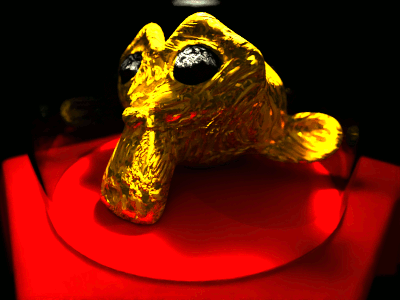
\includegraphics[width=\linewidth]{Medien/suzanne-raw}
				\caption{Raw}
			\end{subfigure}
			\begin{subfigure}{0.32\linewidth}
				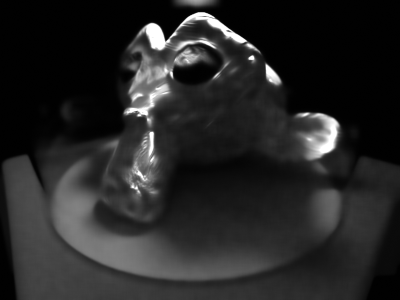
\includegraphics[width=\linewidth]{Medien/suzanne-intensity}
				\caption{Intensität}
			\end{subfigure}
			\begin{subfigure}{0.32\linewidth}
				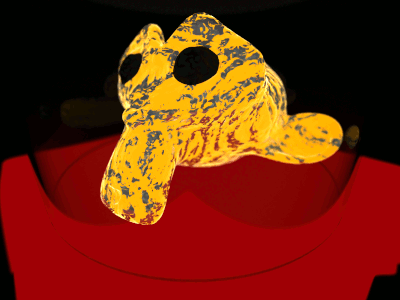
\includegraphics[width=\linewidth]{Medien/suzanne-albedo}
				\caption{Albedo}
			\end{subfigure}
			\begin{subfigure}{0.32\linewidth}
				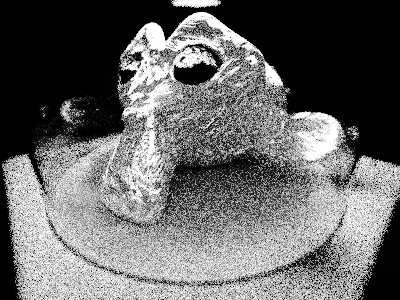
\includegraphics[width=\linewidth]{Medien/suzanne-variance}
				\caption{Varianz}
			\end{subfigure}
			\hfill
			\begin{subfigure}{0.32\linewidth}
				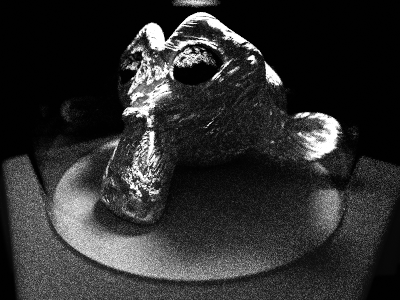
\includegraphics[width=\linewidth]{Medien/suzanne-sw}
				\caption{Schwarz-Weiß}
			\end{subfigure}
			\hfill
			\begin{subfigure}{0.32\linewidth}
				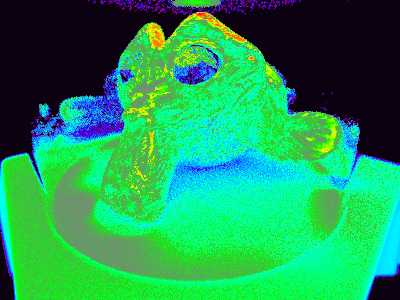
\includegraphics[width=\linewidth]{Medien/suzanne-false-color}
				\caption{Falschfarben}
			\end{subfigure}
			\caption[Suzanne in verschiedenen Renderpasses]{Suzanne, das Maskottchen von Blender mit Goldmaterial in verschiedenen Render-Passes}
			\label{fig:suzanne}
		\end{figure}
		\autoref{fig:suzanne} besteht aus mehreren Teilen, die mit  \lstinline[language=thesis-latexbeispiel]|\begin{subfigure}{0.33\linewidth}| in die \lstinline[language=thesis-latexbeispiel]|figure|-Umgebung aufgenommen werden können. 
		\lstinline[language=thesis-latexbeispiel]|0.33\linewidth| gibt dabei an, dass die Breite der eingefügten Unterabbildung \SI{33}{\percent} der aktuellen Textbreite entsprechen soll.
		
	\section{Tabellen}
		\autoref{tab:beispiel} zeigt eine beispielhafte Tabelle.
		Tabellen werden in der \lstinline[language=thesis-latexbeispiel]|table|-Umgebung gesetzt und sind genau wie Abbildungen \emph{float}-Objekte (siehe \autoref{sec:wissen:float}).
		Die eigentliche Tabelle kann dann \zb{} mit der \lstinline[language=thesis-latexbeispiel]|tabular|-Umgebung gesetzt werden.
		\LaTeX-Editoren wie \emph{TeXstudio} bieten benutzerfreundliche Hilfmittel zur Bearbeitung und automatischen Quelltextformatierung von Tabellen, falls man im Quelltext den Überblick verlieren sollte.
		\begin{table}[bh]
			\centering
			\begin{vorlagenbeispiel}
				\begin{tabular}{l|cr} % lcr: jeder Buchstabe steht für eine Spalte, | erzeugt ein vertikale Linie
					(l)eft  & (c)enter & (r)ight \\ % Spalten werden mit & getrennt, Zeilen mit \\ beendet
					\hline                          % \hline erzeugt eine horizontale Linie
					Hier    & steht    & etwas   \\
					in      & einer    & Tabelle \\
					\hline
					Das hier & steht & weiter unten\\
					Text kann auch & \multicolumn{2}{c}{über mehrere Spalten gehen}
				\end{tabular}
			\end{vorlagenbeispiel}
			\caption{Beispiel zu Tabellen}
			\label{tab:beispiel}
		\end{table}
		\begin{lstlisting}[language=thesis-latexbeispiel]
\begin{table}
	\centering
	\begin{tabular}{l|cr}
		(l)eft  & (c)enter & (r)ight \\
		\hline                         
		Hier    & steht    & etwas   \\
		in      & einer    & Tabelle \\
		\hline
		Das hier & steht & weiter unten\\
		Text kann auch & \multicolumn{2}{c}{über mehrere Spalten gehen}
	\end{tabular}
	\caption{Beispiel zu Tabellen}
	\label{tab:beispiel}
\end{table}
		\end{lstlisting}
		
		
	\section{Quellcode}
		\emph{Für Quellcode nutzt diese Vorlage das Paket \lstinline|listings|.}
		\medskip
		
		Mit \lstinline{\lstinline[language=C]|printf("%d", 42);|} kann Quellcode, z.B. \begin{vorlagenbeispiel}
		\lstinline[language=C]|printf("%d", 42);|
		\end{vorlagenbeispiel} mitten im Text gesetzt werden.
		Der optionale Parameter \lstinline[language=thesis-latexbeispiel]|language=C| gibt dabei an, dass der gezeigte Code in der Programmiersprache \emph{C} vorliegt.
%		
		Die Dokumentation des \lstinline[language=thesis-latexbeispiel]|listings|-Paketes enthält eine vollständige Liste der vordefinierten Programmiersprachen.
		Es gibt ausserdem die Möglichkeit Syntaxhighlighting für weitere Sprachen selber zu definieren.
		\bigskip
		
		Einen abgesetzten Code-Block erzeugt man mit \lstinline[language=thesis-latexbeispiel]|\begin{lstlisting}[language=C]|. Es ist auch möglich Quellcode-Dateien direkt einzubinden (\lstinline[language=thesis-latexbeispiel]|\lstinputlisting{/pfad/zum/quell.code}|), nur einen bestimmten Ausschnitt des Quellcodes anzuzeigen oder die Zeilennummerierung anzupassen (siehe \autoref{code}).
		
		\begin{vorlagenbeispiel}
			\begin{lstlisting}[label=code, language=C, caption={Hello World-Beispiel im lstlisting-Beispiel},firstnumber=1234, emph={printf, schokostuecke}] 
#include <stdio.h>    // Für printf/scanf etc.
#include <stdlib.h>   // Speicherverwaltung & EXIT_SUCCESS/EXIT_FAILURE-Makros

int main(void){
	printf("Hallo LaTeX!\n"); // Textausgabe-Beispiel
	return EXIT_SUCCESS;
}

// In dieser Vorlage sind auch ä,ö,ü,ß und Ä,Ö,Ü erlaubt
			\end{lstlisting}
		\end{vorlagenbeispiel}
		
		Neben \lstinline|language| gibt es noch weitere optionale Parameter, mit denen das Erscheinungsbild angepasst werden kann.
		In \autoref{code} wurden \lstinline|label=labelname| (kann man referenzieren), \lstinline|caption={Beschriftung des Quellcode-Blocks}| und \lstinline|firstnumber=1234| zum Anpassen der Zeilennummerierung verwendet.
	
	\section{Labels \& Referenzen}\label{label-name}
		Überschriften, Abbildungen, Tabellen usw. werden von \LaTeX{} automatisch nummeriert.
		
		Will man auf einen bestimmten Textabschnitt oder z.B. auf eine Grafik verweisen, so setzt man am Ziel ein \lstinline|\label{labelname}| und referenziert dieses dann mit \lstinline|\ref{labelname}|.
		\lstinline|\autoref{labelname}| ergänzt automatisch den Typ des referenzierten Objekts:
		
		\begin{vorlagenbeispiel}
		Wenn ich den aktuellen Abschnitt mit \lstinline|ref| referenziere, ergibt sich \ref{label-name} (also nur die Nummer), nutzte ich \lstinline|\autoref{labelname}]| ist auch der Typ des Objekts mit dabei: \autoref{label-name}.
%		
		Es ist natürlich auch möglich, \autoref{code} oder \autoref{fig:beispiel} zu referenzieren.
		\end{vorlagenbeispiel}
		
		Mit dem Befehl \lstinline|\nameref{labelname}| erhält man statt der Nummer den Namen des referenzierten Objekts:
		
		\begin{vorlagenbeispiel}
			Der aktuelle Abschnitt hat die Nummer \ref{label-name} und heißt \enquote{\nameref{label-name}}.
		\end{vorlagenbeispiel}
		
		\begin{lstlisting}[language=thesis-latexbeispiel]
Der aktuelle Abschnitt hat die Nummer \ref{label-name} und heißt \enquote{\nameref{label-name}}.
		\end{lstlisting}
		
		Mit \lstinline|\pageref{labelname}| erhält man die Seitennummer des referenzierten Objekts:
		
		\begin{vorlagenbeispiel}
			Dieser Abschnitt beginnt auf Seite \pageref{label-name}.
		\end{vorlagenbeispiel}
			
	\section{URLs}
		Mit \lstinline[language=thesis-latexbeispiel]|\url{https://www.blender.org}| lassen sich URLs setzen, die man im PDF dann auch anklicken kann. Der dezente Rahmen um den Link herum wird lediglich am Bildschirm angezeigt, beim Drucken aber nicht mit ausgedruckt.
		
		\begin{vorlagenbeispiel}
			Die Open-Source Software Blender (\url{https://www.blender.org}) ist ein mächtiges Allround-Werkzeug für die Erstellung von 3D-Grafik, welches unter anderem die Bereiche Modellierung, Texturierung, Rendering, Rigging, Physik-Simulation, Partikelsimulation, Sculpting, Animation, Videotracking, Videobearbeitung, Compositing und Skripting abdeckt.
		\end{vorlagenbeispiel}
		\medskip

		Will man einen Link im PDF setzen, statt der URL aber einen anderen Text anzeigen, ist dies mit \lstinline[language=thesis-latexbeispiel]|\href{url}{text}| möglich:
%		
		\begin{vorlagenbeispiel}
			Mit dem sogenannten \href{https://www.blender.org/features/grease-pencil/}{Grease Pencil}-Werkzeug können Künstler 2D Zeichnungen in einer 3D Umgebung erstellen.
			Ursprünglich lediglich ein einfaches Werkzeug für Anmerkungen (daher der Name) wurde es seit \href{https://www.blender.org/download/releases/2-73/}{Blender Version 2.73} zu einem deutlich mächtigeren Werkzeug zur Animation im 2D-Stil weiterentwickelt.
		\end{vorlagenbeispiel}		
		
	\section{Glossareinträge \& Symbole}
		\emph{Für Glossareinträge und Symbole nutzt diese Vorlage das Paket \lstinline|glossaries-extra|}
		\medskip
		
		\subsection{Glossar}
			Glossareinträge werden in der Datei \lstinline|Glossar.tex| definiert. Mit \lstinline[language=thesis-latexbeispiel]|\gls{labelname}| können sie im Text verwendet werden:
			
			\begin{vorlagenbeispiel}
				Es gibt ganz tolle \gls{crc}-Algorithmen, die eine \gls{crc} genau nach dem Schema typischer \glspl{crc} berechnen.
				Hier ist ein \gls{ex} für einen Glossar-Eintrag. 
				Und hier noch die tolle Abkürzung \gls{svm}, \gls{bspw} stehend für \gls{svm}.
			\end{vorlagenbeispiel}
			
			Manchmal passt der Originaltext des Glossareintrags grammatikalisch nicht in den Text, es soll aber trotzdem ein Eintrag erzeugt werden.
			In diesem Fall kann mit 			\lstinline[language=thesis-latexbeispiel]|\glslink{labelname}{text}| ein alternativer Text angegeben werden:
			
			\begin{vorlagenbeispiel}
			Das Gebiet der \gls{rekursion} beschäfigt sich mit \glslink{rekursion}{rekursivem} Verhalten.
			\end{vorlagenbeispiel}
		\subsection{Symbole}
			Mathematische und physikalische Symbole können ebenfalls in der \lstinline|Glossar.tex| angegeben werden.
			Im Text werden sie mit \lstinline[language=thesis-latexbeispiel]|\glssymbol{labelname}| angesprochen\footnote{Mit \textbackslash gls würde lediglich ihr Name ausgegeben}:
%			
			\begin{vorlagenbeispiel}
				Die ersten drei Buchstaben des griechischen Alphabets sind \glssymbol{alpha}, \glssymbol{beta} und natürlich \glssymbol{gamma}. Die Leere Menge wird mit \glssymbol{emptyset} notiert.
			\end{vorlagenbeispiel}
			
	\section{Todos}
		Solange die Thesis noch nicht fertig ist, wird man immer mal wieder \enquote{Todos} haben, also Dinge, die noch zu erledigen sind.
		Dank dem \LaTeX-Paket \lstinline[language=thesis-latexbeispiel]|todonotes| kann man diese ganz einfach mit \lstinline[language=thesis-latexbeispiel]|\todo{Hier ist noch etwas zu tun}|\todo{Hier ist noch etwas zu tun} hinzufügen.
%		
		Mit \lstinline[language=thesis-latexbeispiel]|\listoftodos| lässt sich eine Liste aller Todos im aktuellen Dokument ausgeben:
		
		\begingroup % ein bisschen Hacking drumherum,
			\let\clearpage\relax %damit keine neue Seite angefangen wird
			\vspace{3em} % aber auch genug Abstand da ist, erst dann kommt
			\listoftodos[Was noch zu tun ist:] % das eigentliche Todo-Verzeichnis
		\endgroup
		
		% Sorry, dieses Paket ist einfach zu gut, als dass ich das weglassen kann ;-)
		\vfill
		\centering
		\begin{tikzpicture}[scale=2]
			\duck[signpost=\scalebox{.9}{\parbox{2cm}{\centering\sffamily Das Ende ist nahe!}}]
		\end{tikzpicture}
		\vfill
		Ende ;-)  % Beispiele zu LaTeX

	%%%%%%%%%%%%%%%%%%%%%%%%%%%%%%%%%%%%%%%%%%%%%%%%%%%%%%%%%%%%%%%%%%%%%%%%%%%%
	%%% ENDE %%% ENDE %%% ENDE %%% ENDE %%% ENDE %%% ENDE %%% ENDE %%% ENDE %%%%
	%%%%%%%%%%%%%%%%%%%%%%%%%%%%%%%%%%%%%%%%%%%%%%%%%%%%%%%%%%%%%%%%%%%%%%%%%%%%
\end{document} 